\documentclass[12pt, italian]{PhdThesis}[2014/09/23]%,UdinePhdThesisCR
\usepackage{babel}
\usepackage[final]{graphicx}

\usepackage{apacite}                                    % Formatta la bibliografia secondo lo standard APA 6.
\usepackage{blindtext}                                  % Genera il Lorem Ipsum per verificare la corretta formattazione.
\usepackage[OT1]{fontenc}                               % Permette la selezione di codifiche di font per il documento garantendo 
                                                        %   anche comandi specifici per famiglia di font.
\usepackage[a4paper, margin=23mm]{geometry}             % Formatta in maniera "semi-automatica" le varie pagine del documento 
                                                        %   permettendo anche l'uso dell'auto-centering.
\usepackage{graphicx}                                   % Manipola in maniera basilare il testo, fornendo colori e grafici.
\usepackage{lipsum}                                     % Genera il Lorem Ipsum trattato come un array di paragrafi. 
\usepackage{natbib}                                     % Genera la bibliografia, generando anche note numerate.
\usepackage{ragged2e}                                   % Formattazione del testo irregolare. 
\usepackage{parskip}                                    % Gestione dell'interlinea tra paragrafi
\usepackage{setspace}                                   % Gesitione dell'interlinea

\usepackage[hyphens]{url}                               % Parametri aggiuntivi per la formattazione dei link
\usepackage{hyperref}                                   %
\hypersetup{breaklinks = true, pdfborder = {0 0 0}}                          % Tramite il pacchetto precedente, permette di mandare a capo i link, 
                                                        %   suddividendoli per trattini

\tolerance=1                                            % Gruppo di comandi che permettono di giustificare il testo, 
\emergencystretch=\maxdimen                             %   aggiungendo spazi bianchi invece di andare a capo.
\hyphenpenalty=10000
\hbadness=10000

\begin{document}

    \frontmatter
    \begin{titlepage}
        \centering
        
\includegraphics[width=4cm]{stemma-nero.png}
        \vspace{1cm}
    
        \textsc{
            \Huge{Università degli Studi di Udine}\newline
            \vspace{0,5cm}
            \rule{\textwidth}{0,5pt}
        }
    
        \vspace{2,5cm}
        \Centering
        \LARGE{Corso di Laurea in Scienze e Tecnologie Multimediali}
        \newline
        \vspace{0,3cm}
        \normalsize{CL-20 CL-31}
        \vspace{1,5cm}
        \newline
        \centering
        
        \huge{\textbf{Figura e ruolo \newline del Tecnico Informatico \newline in un Polo Universitario}}
        % matricola in caso se c'è spazio

        \vspace{3,5cm}
        \Large{\begin{flushleft}
            \textsl{Relatore:}\hfill\textsl{Laureando:}
            \newline
            Prof. Niki Martinel \hfill Pietro Furlan
        \end{flushleft}}
        \Centering
        \vspace{1cm}
        \textsc{Anno Accademico: 2024/2025}
        
    \end{titlepage}

\thispagestyle{empty}
\newpage
\onehalfspacing

    \begin{dedication}
        \itshape{
            Ringrazio il Prof. Niki Martinel \\ per essere stato mio Relatore e Tutor di tirocinio. \\ \hfill \break
            Ringrazio Mary, Roberto, Agnese, Eleonora. \\
            Grazie anche a Susj, Frank, \\ Mirella e Giovanni, Flora e Francesco.
        }
    \end{dedication}
    
    \begin{abstract}
            The proposed thesis will focus on the figure and role of the IT Technician in a University Campus based upon the curricular internship at Gorizia Multipurpose Center (CEGO). The thesis has been organized into several chapters, each of which has been divided into paragraphs to better provide information regarding the development of said internship and to appropriately outline the role of the IT Technician.
            The first chapter serves as the introduction to the description of the CEGO and discusses the key roles within it through interviews conducted in person and remotely via the Microsoft Teams platform. The differences between the CEPO and the CEGO are described afterwards in a separate paragraph to better illustrate them. 
        \par
            Immediately after the introductory chapter, the devices are then listed that may be encountered, the role of those devices is described within the physical topography of CEGO's multimedia classrooms. 
            The various tasks of the IT Technician are explained next, distinguishing between those related to collaboration in IT and multimedia management, those related to the maintenance of IT and audiovisual systems, and finally, those of a more general nature that cannot easily be classified into these two categories.
        \par
            Thus a chapter will be dedicated to discussing the future of the IT Technician role in a digital world increasingly dominated by Artificial Intelligence. This chapter will also illustrate how the dynamics between the two entities can be resolved by proposing possible solutions for coexistence.
        \par
            Adequate space is also given to the results obtained from the interventions during the internship and how these can impact the quality of the services offered within CEGO, as well as at a University Campus. This section also discusses how the Bachelor Degree in Multimedia Science and Technology (CL-20 CL-31) prepares for future IT/multimedia technicians and maintenance workers, as well as Teachers for the B016 Computer Science and Technology Laboratories competition class, as required by current legislation.
        \par
            The thesis concludes with a summary of the key points regarding the IT Technician and their role within a university, as well as a reflection on the interventions and tools encountered.
    \end{abstract}
    
    \frontmatter
    \partstyle{serifbig}
    \chaptertitlestyle{serifbig}
    \pagestyle{serif}
    \justifying
        \renewcommand * \contentsname{Sommario}                 % Rinomina il Sommario da "Tables of Content" in "Sommario"
        \tableofcontents
        \listoffigures
        
% ---------------------------------------------------------------------------------------
    \introduction\label{ch:intro}
        Nell'era digitale la figura del Tecnico Informatico è diventata oramai onnipresente ed è spesso fondamentale per il corretto funzionamento di aziende e di istituzioni. Le università in particolare necessitano della figura del Tecnico Informatico in quanto molti servizi offerti, se non tutti, prevedono componenti trasmesse per via informatica. \newline
        Il Tecnico Informatico è appunto quella figura che permette il corretto funzionamento dell'intera rete locale dell'Università e che sostiene il Corpo Docente e il personale amministrativo nell'utilizzo delle attrezzature informatiche, multimediali e/o audiovisive presenti negli spazi gestiti dall'Università di Udine.
    \par
        La presente Tesi di Laurea, nata dall'elaborazione dell'esperienza maturata in sede di tirocinio curricolare (9 CFU) presso la sede di Ateneo a Gorizia, tratta della figura e del ruolo del Tecnico Informatico all'interno di un Polo Universitario, soffermandosi principalmente sulla collaborazione alla gestione informatica e multimediale nonché sulla manutenzione degli impianti audiovisivi, presenti nel Centro Polifunzionale di Pordenone (CEPO) e nel Centro Polifunzionale di Gorizia (CEGO). \newline
        Per approfondire questo aspetto sono state condotte alcune interviste alle figure-chiave del CEGO che si sono gentilmente rese disponibili all'indagine. 
% ---------------------------------------------------------------------------------------
    \subsection*{Struttura dell'elaborato}
        \par
            L'elaborato proposto è stato organizzato in diversi capitoli, ognuno dei quali è stato suddiviso in paragrafi per meglio fornire le informazioni relative allo sviluppo del tirocinio curricolare e per delineare opportunamente la figura e il ruolo del Tecnico Informatico. 
        \par
            Il primo capitolo, immediatamente successivo a questa introduzione, costituisce la premessa alla descrizione del CEGO e tratta quali siano le figure principali al suo interno attraverso opportune interviste svolte sia in presenza che da remoto tramite la piattaforma Teams. Vengono quindi descritte le differenze tra il CEPO e il CEGO in un paragrafo a sé stante. \newline
            Di seguito sono elencati i dispositivi che si possono incontrare e si descrive il loro ruolo all'interno della topografia fisica degli impianti del CEGO. 
        \par
            Trattando la figura e il ruolo del Tecnico Informatico ne vengono spiegate le varie mansioni, distinguendo tra quelle relative alla collaborazione dalla gestione informatica e multimediale, quelle relative alla manutenzione degli impianti informatici e audiovisivi e, infine, quelle di natura più generale, non facilmente riconducibili a queste due macro categorie.
        \par
            Proseguendo, verrà dedicato un capitolo alla discussione sul futuro della figura del Tecnico Informatico in un mondo digitale sempre più dominato dalle Intelligenze Artificiali. In tale capitolo si illustreranno anche come si potrebbero risolvere le dinamiche tra le due entità, proponendo anche possibili soluzioni di mediate. 
        \par
            Adeguato spazio viene dedicato inoltre ai risultati ottenuti dagli interventi durante il tirocinio e come questi possano impattare la qualità dei servizi offerti all'interno del CEGO, nonché in un Polo Universitario.
            In questa sezione si fa riferimento anche a come il Corso di Laurea in Scienze e Tecnologie Multimediali (CL-20 CL-31) prepari i futuri tecnici e manutentori del settore informatico/multimediale nonché gli insegnanti Tecnico Pratici della classe di concorso B016, Laboratori di scienze e tecnologie informatiche, come previsto dalla normativa vigente.
        \par
            In conclusione alla Tesi di Laurea, vengono riassunti i punti principali della figura del Tecnico Informatico e del suo ruolo all'interno di un Polo Universitario, nonché una riflessione sugli interventi e i dispositivi incontrati.
% ---------------------------------------------------------------------------------------
    \subsection*{Obiettivo}
        \par
            L'obiettivo dell'elaborato è quello di descrivere il ruolo del Tecnico Informatico presso un Polo Universitario e di come il suo ruolo in loco, spesso poco considerato quando si parla di informatica generale, sia invece fondamentale per garantire la continuità dei servizi TIC (Tecnologie dell'Informazione e della Comunicazione) offerti e di garantirne la maggiore qualità possibile a tutti gli utenti. 
% -------------------------------------------------------------------------------------- 
    \subsection*{Contesto e Motivazioni}
        \par
            La figura del Tecnico Informatico è spesso tralasciata nei discorsi di settore in quanto è una figura onnipresente e discreta; tuttavia risulta fondamentale per poter garantire continuità dei servizi offerti e qualità più alta. È altamente necessaria soprattutto in un Polo Universitario, in quanto molti dei servizi che vengono ad oggi offerti risultano composti dalla parte telematica che informatica.
    
% --------------------------------------------------------------------------------------- 
    \mainmatter
    \setcounter{chapter}{1}

\chapter{Organizzazione}
    \par
        L'Università degli Studi di Udine offre i suoi insegnamenti in due sedi distaccate, situate rispettivamente a Pordenone e a Gorizia. \newline
        Entrambe fanno riferimento alla Direzione Centri e Servizi (DICS) e svolgono funzioni di supporto alle attività di Ateneo, alla gestione delle carriere degli studenti e ai servizi alla didattica, attraverso strutture dell'Amministrazione Centrale (AMCE) o dei Dipartimenti. \newline
        Le segreterie dei due Centri lavorano a stretto contatto con gli Enti Territoriali promuovendo l'Ateneo sul territorio e più in generale coltivando i rapporti con gli altri Enti pubblici e privati esistenti. \newline
        Entrambe operano secondo le indicazioni del Responsabile DICS e dei Delegati del Rettore, sulla base dei Regolamenti di Funzionamento\footnote{\cite{IstruzioniCEGO-CEPO}}. \newline
        Nonostante i compiti diversificati, ogni membro della Direzione del CEGO lavora all'unisono per garantire la continuità del servizio che viene offerto dall'Università. 
        Durante il tirocinio da me svolto ho avuto l'occasione di interfacciarmi con una realtà complessa come può esserlo l'organizzazione di un Polo Universitario, avvicinandomi alla componente umana dell'organizzazione del CEGO. 
% ---------------------------------------------------------------------------------------
    \section{Organigramma del Centro Polifunzionale di Gorizia}
        \par
            Ciascuna intervista al personale del CEGO è stata condotta utilizzando due domande di riferimento: "Qual è il suo ruolo all'intero del CEGO?" e "In relazione alla domanda precedente, quali mansioni ricopre il suo ruolo?". 

            Per maggior chiarezza, si ritiene opportuno esplicitare alcune righe: 
            \begin{itemize}
                \item \textit{DICS}: DIrezione Centro e Servizi;
                \item \textit{AMCE}: AMministrazione Centrale;
                \item \textit{DIAF}: DIrezione Amministrativa e Finanza;
                \item \textit{ADID}: Area servizi per la DIDattica;
                \item \textit{ASTU}: Area servizi agli STUdenti;
                \item \textit{ALOG}: Area edilizia e LOGistica;
                \item \textit{DISO}: ufficio DIritto allo StudiO;
                \item \textit{DAGS}: Direzione Acquisti, Gare e Servizi in outsorucing;
                \item \textit{DARU}: Direzione Risorse Umane e Affari generali;
                \item \textit{DIPC}: DIrezione Pianificazione, Controllo e valutazione;
                \item \textit{DIP}: DIPartimento; 
                \item \textit{CCS}: Consiglio del Corso di Studio;
                \item \textit{CDD}: Consiglio Di Dipartimento;
                \item \textit{CdS}: Corso di Studio;
                \item \textit{L}: Laurea Triennale; 
                \item \textit{LM}: Laurea Magistrale;
                \item \textit{SPES}: Servizio di Posta Elettronica per gli Studenti;
                \item \textit{Scheda SUA}: Scheda Unica Annuale;
            \end{itemize}
            Un elenco più completo si può reperire nella pagina web \cite{AcronimiSigle} dell'Università degli Studi di Udine. \newline
            Da precisare che il CEGO opera in due poli diversi, il primo è ubicato presso Via Santa Chiara 1/A mentre il secondo, distante pochi metri, si trova nel Corso Verdi al civico 4. Entrambi sono situati nel centro di Gorizia. 
% ---------------------------------------------------------------------------------------
        \subsubsection{Prof.ssa Renata Kodilja - Delegata del Rettore}
            La Prof.ssa Renata Kodilja, Delegata del Rettore, ricopre anche la delega alla Direzione del CEGO, che corrisponde alla presa in carico delle relazioni con il territorio, nello specifico con gli Enti e le Istituzioni del Sistema Gorizia che concorrono a  finanziare la presenza dell'Università nel territorio. Inoltre si occupa della gestione del funzionamento interno dell'aspetto di \textsl{governance} e delle strategie d'uso degli spazi. Nell'eventualità che si verifichi una carenza degli spazi, la Delegata cerca soluzioni e provvede a contratti e a convenzioni che coprano il fabbisogno dell'utenza accolta  dall'Ateneo\footnote{Questo implica il fatto che il numero massimo di immatricolazioni dipenda direttamente dalla disponibilità delle aule. Ad oggi il numero massimo di matricole corrisponde a 230, cui si aggiungono 20 matricole di provenienza extra Europea.}. \newline
            Per quanto riguarda le relazioni con il territorio questo significa invece governare i patti e gli accordi o le convenzioni con gli Enti che sostengono, finanziano, hanno interesse, motivazione e attenzione per far sì che l'Università sia a Gorizia. A queste interlocuzioni partecipano due controparti principali: il Consorzio per lo Sviluppo del Polo Universitario di Gorizia (CONSUNIGO), di cui è presidente l'Avv. Sergio Orzan\footnote{\cite{CONSUNIGO}}, e il Consorzio Universitario di Pordenone (UNIPORDENONE), di cui è presidente il Dott. Paolo Candotti. Questi Consorzi ospitano le due Sedi dell'Università degli Studi di Udine in Friuli-Venezia Giulia, mentre la Sede di Gemona non usufruisce del sostegno di alcun Consorzio. \newline
            CONSUNIGO e UNIPORDENONE raccolgono i finanziamenti e si interfacciano con la Sede Universitaria per sostenerne la didattica e il funzionamento. Il CONSUNIGO gestisce in buona misura i contratti per le docenze temporanee, mentre le spese per il mantenimento e il funzionamento delle strutture sono gestite direttamente dall'Università. \newline
            Un altro finanziatore importante è la Cassa di Risparmio di Gorizia (CARIGO) la cui missione è quella di sviluppo e promozione del territorio, mantenendo la compresenza dei due Atenei della Regione. 
            Si aggiungono la Camera di Commercio, Industria, Artigianato e Agricoltura Venezia Giulia (CCIAA Venezia Giulia Trieste Gorizia)\footnote{\cite{CCIAA}}, che accorpa le Camere di Commercio di Venezia e Trieste; i Gruppi Europei di Cooperazione Territoriale (GECT)\footnote{\cite{GECTGOEZTS}} per la città di Gorizia, ossia il consorzio tra le città di Gorizia, Nova Gorica e San Pietro-Vertoiba, che accoglie e gestisce i fondi europei per lo sviluppo e l'integrazione transfrontaliera, finanziando progetti di integrazione transfrontaliera e progetti Interreg EU.
% ---------------------------------------------------------------------------------------
        \subsubsection{Dott.ssa Cristina Prizzi - Funzionaria Amministrativa (Capocentro)}
            La Dott.ssa Cristina Prizzi, Funzionaria Amministrativa, ha due ruoli principali: supportare e collaborare con la Prof.ssa Kodilja in tutte le sue attività da Delegata del Rettore, nello specifico nei rapporti con enti pubblici, nei rapporti con i finanziatori, in presenza a determinati eventi e occupandosi della stesura di verbali. La sua figura funge anche da ponte tra gli uffici della Sede Centrale e il resto del CEGO presente nel polo di Santa Chiara. È la responsabile e la coordinatrice del personale, di conseguenza della sede, verificandone il buon andamento. Sempre in relazione agli enti, funge anche come punto di riferimento, trasmettendo le richieste di finanziamento e altro materiale. \newline
            In secondo ruolo, la Dott.ssa Prizzi svolge anche mansioni di categoria organizzativa, lavorando a più che stretto contatto con la Delegata per monitorare l'effettivo svolgimento dei vari compiti.
% ---------------------------------------------------------------------------------------
        \subsubsection{Dott.ssa Cristina Delmonaco - Referente del Corso di Laurea Relazione Pubbliche (CL-20)}
            La Dott.ssa Cristina Delmonaco si occupa della didattica e della logistica del Corso di Laurea Relazioni Pubbliche, corso tenuto solamente nella Sede di Gorizia; nello specifico organizza l'attribuzione delle aule agli insegnamenti e i calendari degli appelli d'esame. \newline
            Inoltre si occupa, in parallelo alla carica di Referente del Corso di Laurea Relazioni Pubbliche, della gestione organizzativa e logistica degli eventi che si svolgono in corso d'anno nel polo di via Santa Chiara o di Corso Verdi. \newline
            In collaborazione con la Dott.ssa Erika Bader, si occupa in parte della Segreteria Studenti. 
% ---------------------------------------------------------------------------------------
        \subsubsection{Dott. Carlo Carratù - Referente amministrativo dei Corsi di Laurea}
            Il Dott. Carlo Carratù si occupa dell'aspetto finanziario per il CEGO e per l'area DICS; gestisce gli ordinamenti didattici e, a cascata, tutto ciò che riguarda le attività normative, ad esempio il piano di studi e i relativi allegati, nonché le eventuali modifiche. Si occupa dei Consigli dei Corsi di Studio, delle Commissioni Qualità, degli orari e degli appelli d'esame per il Corso di Laurea Discipline dell'audiovisivo, dei media e dello spettacolo (DAMS; CL-3) nonché dell'inserimento nei vari moduli U-GOV e della scheda SUA. Quest'ultima è uno strumento gestionale del Ministero dell'Università e della Ricerca, funzionale alla progettazione, alla realizzazione, all'autovalutazione e alla ri-progettazione del CdS. La scheda mira a definire la domanda di formazione, esplicitare l'offerta formativa, certificare i risultati di apprendimento, chiarire i ruoli e le responsabilità che attengono alla gestione del sistema di Assicurazione della Qualità dell'Ateneo oltre che riesaminare periodicamente l'impianto del CdS e i suoi effetti per apportare le necessarie modifiche\footnote{\cite{schedaSua}}. 
% ---------------------------------------------------------------------------------------
        \subsubsection{Dott.ssa Cristina Feresin - Ufficio Tirocini}
            La Dott.ssa Cristina Feresin segue l'organizzazione dei tirocini curricolari e volontari per gli studenti, fornisce le indicazioni sulle procedure e sulle pratiche di tirocini dal primo inserimento in azienda fino alla chiusura, funge da referente per i tirocini interni e fornisce anche un \textsl{helpdesk} per i tirocini, rivolto sia agli studenti sia alle aziende. Inoltre organizza l'incontro obbligatorio per i tirocini del Corso di Laurea Relazioni Pubbliche. La Dott.ssa è anche membro della Commissione Tirocini, lavorando in stretta collaborazione con l'Ufficio Tirocini della Sede di Udine.\newline
            Infine promuove tra gli studenti gli avvisi relativi alla ricerca di personale altamente qualificato da parte delle aziende e fornisce supporto alla Segreteria della Direzione. 
% ---------------------------------------------------------------------------------------
        \subsubsection{Dott. Andrea Castelli - Supporto IT}
            Il Dott. Andrea Castelli fornisce assistenza tecnica soprattutto agli Uffici Amministrativi ma anche al resto dei dipendenti, dei professori, degli studenti. L'assistenza fornita è generale e copre ogni aspetto dell'ambito informatico d'Ateneo: reti internet, computer, stampanti, scanner, etc. Inoltre installa i nuovi software utili al corretto e migliore andamento dei dispositivi.
% ---------------------------------------------------------------------------------------
        \subsubsection{Dott. Francesco Barreca - Tecnico Multimediale}
            Il Dott. Francesco Barreca lavora come tecnico multimediale e specialista in didattica a distanza dell’Università degli Studi di Udine. Il Dott. Progetta e segue la manutenzione degli impianti multimediali delle aule, occupandosi di tutto ciò che riguarda la proiezione, i monitor, l'impianto audio e i sistemi per la didattica online; gestisce la piattaforma di e-learning dell'Ateneo basata su Moodle e la piattaforma dedicata alle registrazioni delle lezioni \emph{uniud.ubicast.tv}; collabora alla realizzazione di eventi istituzionali come l'Inaugurazione dell'Anno Accademico, la Cerimonia del Tocco, lo Student Day e il PhD Day. \newline
            Inolte si occupa della coordinazione tra le ditte esterne in outsourcing, le quali forniscono supporto tecnico per convegni e conferenze; tali ditte si occupano anche della manutenzione delle aule didattiche e curano l'installazione di nuovi impianti multimediali negli spazi di attuali o future sedi universitarie.
% ---------------------------------------------------------------------------------------
        \subsubsection{Dott. Lino Saro - Funzionario Informatico}
            Il Dott. Lino Saro si occupa della didattica laboratoriale, dell'allestimento dei laboratori informatici compresi i server CUDA, della piattaforma Moodle Learning Management System (LMS) e dei vari servizi e-learning. Prepara la correzione automatica dei vari programmi, è membro della Commissione dell'Alfabetizzazione Informatica per gli Studenti. \newline
            In parte, gestisce l'amministrazione del servizio Active Directory (AD) di Ateneo, i domini e le varie tabelle DNS; costruisce i vari bandi per i concorsi che utilizzano le piattaforme online LMS per entrare a lavorare in università: nello specifico questo si traduce nel preparare gli account temporanei per l'accesso ai test d'ammissione. Struttura sia la prova stessa sia il corso; tutta la preparazione viene anche sottoposta ad un controllo incrociato con gli account che poi verranno utilizzati per fare il test. \newline
            Lavora a stretto contatto con colleghi sviluppatori di software in base alle esigenze dell'Ateneo, utilizzando principalmente linguaggi del tipo \textsl{C\#} mentre i colleghi gestiscono applicativi del tipo Esse3 e Xform su richiesta dei Dipartimenti e dell'AMCE, verificando le firme digitali per la didattica e la gestione dei protocolli. Infine il Dott. Saro collabora con i Tecnici che gestiscono i server e i vari dispositivi delle reti e reti wireless, firewall e sicurezza. 
% ---------------------------------------------------------------------------------------
        \subsubsection{Dott.ssa Grazia Puiatti - Bibliotecaria}
            La Dott.ssa Grazia Puiatti è referente della Biblioteca della Sede di Gorizia, quindi si occupa dei prestiti e delle restituzioni dei volumi intrateneo e intrabiblioteche, entrambi tramite la Piattaforma Alma. Sovrintende alla catalogazione, all'inventario della Sede, alla gestione di ordini magazzino e di cancelleria. Tramite la piattaforma Udiscover informa l'utenza del catalogo multimediale e fornisce consulenza bibliografica. \newline
            Gestisce inoltre gli utenti interni ed esterni, preparando e posizionando il materiale informativo. Si occupa della gestione di Tutor e dei vari Collaboratori Studenteschi, lavorando a stretto contatto con la Dott.ssa Feresin per il coordinamento dei tirocinanti.
% ---------------------------------------------------------------------------------------
        \subsubsection{Gabriele Marcatti - Aiuto Bibliotecario}
            Il Sig. Gabriele Marcatti si interfaccia con gli utenti della Biblioteca di Gorizia, gestendo i prestiti e le restituzioni, sia quelli nella Sede sia quelli intrateneo che quelli intrabibliotecari, tramite la Piattaforma Alma. Controlla il corretto allestimento degli scaffali, dell'archivio, delle etichette per le collocazioni, delle timbrature dei libri e infine della stampa del materiale informativo. 
% ---------------------------------------------------------------------------------------
        \subsubsection{Dott.ssa Erika Bader - Referente Segreteria Studenti}
            La Dott.ssa Erika Bader segue la carriera degli studenti dall'orientamento in entrata e le immatricolazioni fino alla compilazione della domanda di Laurea e alla restituzione del Tesserino; aiuta nella compilazione dei Piano di Studio, rilascia i certificati di partecipazione ad eventi, interviene negli incontri mirati alla stesura di Tesi di Laurea e fornisce supporto all'accesso dei test d'ingresso.
% ---------------------------------------------------------------------------------------
        \subsubsection{Prof. Andrea Mariani - Coordinatore DAMS}
            Il Prof. Andrea Mariani coordina il Corpo Docenti e monitora l'andamento della didattica e delle carriere. Svolge anche il ruolo di Docente del Corso di Studi in "Teorie Critiche dei Media e dei Nuovi Media" ed è delegato all'orientamento e all'internazionalizzazione. \newline
            In parallelo al ruolo di Coordinatore e Docente, il Prof. è anche ricercatore in "Archeologia dei Media"\footnote{\cite{AndreaMariani}}. È responsabile e direttore dei progetti che si svolgono nel laboratorio di \textsl{Digital Storytelling} presso la Sede del Dipartimento di Studi Umanistici e del Patrimonio Culturale (DIUM). Tali progetti possono coinvolgere gli studenti come tirocinanti ma sono principalmente mirati all'attività di formazione, organizzata in workshop di vario livello, rivolta a insegnanti, a professionisti e a lavoratori che vogliano acquisire strumenti di comunicazione efficaci e innovativi\footnote{\cite{DigitalStorytellingLAB}}.
            Lavora a stretto contatto con il Dott. Carratù per la costruzione dell'orario didattico delle lezioni e della pianificazione degli appelli d'esame, oltre che per la calendarizzazione della didattica integrativa comprensiva di seminari ed eventi. Collabora con la Dott.ssa Feresin per la gestione dei tirocini curricolari. 
% ---------------------------------------------------------------------------------------
    \section{Differenze tra CEPO e CEGO}
            Le differenze principali tra CEPO e CEGO si possono dividere in due categorie principali: la gestione dei Regolamenti interni e la gestione della Didattica, ma non mancano anche alcuni tratti in comune. \newline
            Le divergenze e convergenze sono state estrapolate dal documento \cite{IstruzioniCEGO-CEPO}. 
% ---------------------------------------------------------------------------------------
        \subsubsection{Gestione dei Regolamenti interni - CEPO}
            La prima principale differenza tra CEPO e CEGO è la gestione dei regolamenti interi, in quanto il CEPO ha mantenuto il regolamento di Funzionamento e, di conseguenza, ha mantenuto l'organo del Consiglio Direttivo. L'aver mantenuto il Regolamento comporta una differenza quasi sostanziale in quanto ne definisce la funzione di organi di competenze e definisce al Consiglio Direttivo delle mansioni da delegare. Altre differenze tra i due Centri polifunzionali si possono trovare in svariati ambiti, tra cui la contabilità e la gestione ordinaria e straordinaria degli immobili. 
% ---------------------------------------------------------------------------------------
        \subsubsection{Gestione della Didattica - CEPO}
            Le gestioni Didattiche del CEPO, come del CEGO, sono in collaborazione funzionale con i Dipartimenti di riferimento dei vari CdS; tuttavia, alcuni di questi CdS sono gestiti in coordinazione con i direttori dei DIP. Va precisato che al CEPO sono presenti diversi CdS tra cui alcuni tenuti da altri Atenei. \newline
            Nello specifico i CdS dell'Università di Udine a Pordenone sono: 
            \begin{itemize} 
                \item \textsl{L - Tecnologie digitali e comunicazione per le industrie creative}: il CEPO ne gestisce il coordinamento funzionale con il Dipartimento delle scienze Matematiche, Informatiche e Fisiche (DMIF), ne gestisce l'orario degli esami e delle lauree nonché il calendario degli appelli, il CEPO ne monitora le pratiche studenti; 
                \item \textsl{LM - Comunicazione Multimediale e Tecnologie dell'Informazione}: CdS gestito in coordinato funzionale con il DMIF; 
                \item \textsl{L - Infermieristica}: CdS gestito dal Dipartimento di MEDdicina (DMED), mentre il CEPO si occupa dei tirocini, dei servizi di supporto alla didattica e alla definizione dell'offerta formativa, oltre al monitoraggio delle pratiche studenti; 
                \item \textsl{L - Ingegneria Industriale dell'Energia}: il CEPO si occupa delle attività di supporto alla didattica in sede, collaborando con il Dipartimento Politecnico di Ingegneria e Architettura (DPIA) e monitorando le pratiche studenti; 
                \item \textsl{LM - Banca e Finanza}: il CEPO si occupa delle attività di supporto alla didattica in sede, collaborando con il Dipartimento di Scienze Economiche e Statistiche (DIES);
            \end{itemize}
            Le equipollenze vengono riconosciute formalmente per tutti i CdS offerti al CEPO: la documentazione necessaria passa attraverso l'organo dell'ASTU che procede con la verifica dei Titoli di Studio. 
        \par
            Il CEPO viene sempre informato dei vari CCS e dei lavori del CDD in caso di impegni a carico del Centro stesso e di cambiamenti facenti riferimento ai vari CdS offerti in sede.\newline
            Ponendo ora il focus i CdS in Tecnologie digitali e comunicazione per le industrie creative e in Comunicazione Multimediale e Tecnologie dell'Informazione, il CEPO segue tutto l'iter delle relative pratiche studenti e procede con la stesura dei verbali di CCS. Inoltre il Centro procede all'informazione, tramite i canali ufficiali, dell'emanazione di bandi relativi alle supplenze e supporta i Docenti nelle possibili problematiche riguardo l'uso della piattaforma Esse3, oltre che nella risoluzione di ogni tipo di problema tecnico si dovesse riscontrare; nel caso di problemi riferiti agli immobili, il CEPO utilizza il \cite{PortaleSelfServiceSysAid}. Per questi due CdS il CEPO definisce anche i calendari degli appelli d'esame e gli Appelli di Laurea con le relative Commissioni, nonché la loro pubblicazione sulle pagine web, dopo essersi confrontato con il DMIF. Per quanto riguarda le Discussioni di Laurea, queste si possono verificare in due spazi principali: in centro città a Palazzo Montereale Mantica, previo consenso del Consorzio, oppure nella sede di Via Prasecco. \newline
            Una precisazione va aggiunta per la LM in Comunicazione Multimediale, in quanto il corso collabora alla gestione del \textit{Double Degree} con l'Università di Klagenfurt, occupandosi al supporto della Commissione didattica per la selezione dei candidati e la pubblicazione dei risultati, nonché il successivo riconoscimento dei Crediti Formativi Universitari conseguiti all'estero. \newline
            Il Centro di Pordenone, infine, si interfaccia con il Centro Linguistico di Ateneo per l'organizzazione di test di piazzamento in sede per le lingue straniere e, successivamente, per l'organizzazione dei corsi delle lingue straniere. Il CEPO ne supporta l'operato per eventuali prove di accertamento organizzate dai CdS. 
% ---------------------------------------------------------------------------------------
        \subsubsection{Gestione dei Regolamenti interni - CEGO}
            Come accennato in precedenza, la gestione dei Regolamenti interni è uno dei due punti fondamentali dove i due centri differiscono; il CEGO, pur essendo una sede a sé stante con un'autonomia diversa rispetto al Centro di Pordenone sotto alcuni punti di vista, fa riferimento direttamente all'Ateneo dato che non utilizza più il regolamento da Centro Polifunzionale. Questo implica una gestione interna degli spazi disponibili tramite i servizi di prenotazione dell'Ateneo e un coordinamento continuo con la Diocesi presente nel polo di Corso Verdi, essendo sotto contratto d'affitto. \newline
            Per quanto riguarda invece le discussioni delle Lauree, queste vengono discusse solamente nel polo di Santa Chiara, lasciando la procedura e la gestione degli spazi completamente in carico al CEGO. 
% ---------------------------------------------------------------------------------------
        \subsubsection{Gestione della Didattica - CEGO}
           L'offerta formativa del CEGO comprende diversi corsi gestiti in coordinazione con i DIP di riferimento, nello specifico: 
            \begin{itemize}
                \item \textsl{L - Relazioni Pubbliche}: fa riferimento al Dipartimento di Lingue e Letterature, Comunicazione, Formazione e Società (DILL);
                \item \textsl{LM - Comunicazione Integrata per le Imprese}: fa riferimento al Dipartimento di Lingue e Letterature, Comunicazione, Formazione e Società (DILL);
                \item \textsl{L - Discipline dell'audiovisivo, dei media e dello spettacolo (DAMS)}: fa riferimento al Dipartimento di studi Umanistici e del Patrimonio Culturale (DIUM).
            \end{itemize}
            I tre CdS sono gestiti dalla Segreteria Didattica in quasi piena autonomia, occupandosi della stesura dei CCS, supportando le attività formative in relazione all'offerta, inserendo i vari regolamenti didattici nella Scheda SUA-CdS e, come nel caso di Pordenone, supportando i docenti nelle eventuali problematiche della piattaforma Esse3. Inoltre il CEGO collabora con la Segreteria ADID per la redazione delle guide e dei Manifesti agli studi dei CdS, aggiustando eventualmente parti del manifesto decise da CCS e/o CDD. \newline
            Dal punto di vista delle lezioni dei vari CdS e dei rispettivi appelli d'esame, la Segreteria Didattica si occupa della creazione e dell'organizzazione dei calendari, pubblicando poi il tutto sulle varie piattaforme. La Segreteria provvede anche della stesura del calendario degli Appelli di Laurea, calendario che viene poi pubblicato sulla piattaforma Esse3. Gli spazi prenotati per lezioni, esami e Lauree vengono gestiti tramite la piattaforma Easyroom. 
% ---------------------------------------------------------------------------------------
        \subsubsection{Caratteristiche in comune e differenze minori}
            \par
                Partendo dalle caratteristiche in comune dei due Centri, entrambi i Responsabili provvedono alle richieste d'acquisto e alla consegna di beni e servizi utili al funzionamento. I Responsabili inoltre sono nominati annualmente agenti contabili del fondo amministrativo assegnato alla rispettiva struttura. 
            \par
                In caso di lavori di manutenzione, periodici o straordinari che siano, è necessario richiedere questi interventi tramite un sistema di ticket fornito dall'università\footnote{\cite{PortaleSelfServiceSysAid}}. L'interfaccia di questo portale differisce tra studente e personale interno mostrando diverse categorie disponibili. Nel caso di uno studente, il portale mostra le seguenti categorie: Esse3, Servizi per gli Studenti, Ricercatori e Dottorati, Tirocini di Medicina, Servizi Informatici e Sistema Qualità di Ateneo. Mentre, nel caso del personale interno, il portale mostra le seguenti categorie: Servizi Informatici, Esse3, DARU, Servizi Tecnici, Area Edilizia e Sistema Qualità di Ateneo. \newline 
                Per quanto riguarda gli interventi di manutenzione edilizia, ogni intervento va comunicato al proprietario della struttura del rispettivo Centro; quindi nel caso del CEPO questi interventi vanno comunicati e concordati con il Consorzio Universitario, mentre nel caso del CEGO bisogna differenziare i due poli: in via Santa Chiara, l'edificio è stato donato dal comune all'Ateneo e quindi gli interventi sono concordati con l'Ateneo stesso, mentre per Corso Verdi ogni intervento, indipendentemente dalla natura, va comunicato e concordato con la Diocesi di Gorizia, in quanto il CEGO è legato all'edificio tramite contratto d'affitto.
            \par
                Entrambi i Centri offrono il servizio di Segreteria Studenti in collaborazione con la segreteria ADID. La comunicazione tra le diverse Segreterie avviene sia in forma scritta sia in presenza in riunioni periodiche. Le Segreterie operano secondo un orario definito dall'Ateneo che garantisca un minimo di giorni in cui siano accessibili agli studenti; è possibile prendere appuntamento e consultare la Segreteria tramite e-mail e telefonicamente.
            \par
                In aggiunta al servizio di Segreteria, entrambi i Centri monitorano la carriera e l'andamento degli studenti sia in entrata che in uscita. In caso di studenti con titolo estero l'ASTU inoltrerà alle Segreterie la documentazione necessaria, aggiornandole sull'iter di verifica dei Titoli di Studio; una volta accertato, il rispettivo Centro procede all'immatricolazione. L'ASTU viene contattato anche per le richieste delle domande di equipollenza e, in particolare per i CdS Tecnologie digitali e comunicazione per le industrie creative e Comunicazione Multimediale e Tecnologie dell'Informazione, il Centro riceve la documentazione necessaria da inoltrare alle Commissioni Didattiche competenti. \newline
                Sia CEPO che CEGO vengono aggiornati annualmente dall'ASTU sugli eventi di orientamento che si svolgeranno, fornisce loro le informazioni necessarie per poter allestire gli spazi ma lasciando ai Centri l'autonomia sulla logistica. I Centri possono anche proporre e ideare degli eventi a livello locale su richiesta dei CdS attivi. A fine di ciascun anno accademico, i Centri creano un report delle attività da inoltrare al Delegato del Rettore in modo da aggiornare il Magnifico Rettore; il CEGO, dopo aver inoltrato il report, lo utilizza per la stipulazione della Scheda SUA. \newline
                Gli studenti delle Lauree Magistrali, iscritti regolarmente, possono partecipare ad un bando di selezione per poter diventare dei Tutor informativi del DIP a cui afferiscono. Entrambi i Centri poi offrono supporto logistico; il CEGO in aggiunta, monitora i tutor nelle attività di orientamento organizzate dai CdS attivi. 
            \par
                Entrambi i Centri offrono la possibilità di seguire dei tirocini sia interni che esterni a tutti gli studenti iscritti a CdS i quali abbiano nel Curriculum l'attività di tirocinio; la sola differenza tra i due è che il CEGO ha un Ufficio Tirocini proprio mentre l'Ufficio Tirocini di riferimento del CEPO ha sede nel Palazzo Toppo Wassermann a Udine, Ufficio referente anche per la Sede Centrale di Ateneo e il Polo distaccato di Gemona.
            \par
                Tra i vari servizi offerti agli studenti, è presente anche il servizio bibliotecario: entrambe le biblioteche presenti nei Centri, operano in collaborazione con l'ABIB e la rete bibliotecaria di Ateneo.
            \par
                Infine, il CEGO ha un sistema di videosorveglianza a capo dell'Ateneo presso il polo di Santa Chiara mentre il sistema del CEPO, nel polo in Via Prasecco, è a capo del Consorzio Universitario. \newline
                CEPO così come CEGO hanno in dotazione personale formato nel primo soccorso e in prevenzione antincendio, personale che segue periodicamente dei corsi di aggiornamento e partecipa alle prove di evacuazione previste dalla normativa vigente. Essendo il CEGO suddiviso in due poli, il personale formato agisce principalmente nel polo di Santa Chiara ma è a disposizione per il polo in Corso Verdi, dato che quella struttura ha il piano delle emergenze affidato alla Diocesi di Gorizia. Anche il personale formato del CEPO partecipa alle prove d'evacuazione che sono organizzate dal Consorzio Universitario. 
% ---------------------------------------------------------------------------------------
    \setcounter{chapter}{2}
\setcounter{section}{0}

\chapter{Dispositivi}
    \par
        Il CEGO offre diversi servizi informatici e multimediali, tra i quali è prevista la possibilità di condividere la schermata di un qualsiasi computer tramite un impianto multimediale ad hoc presente, in diverse misure, in tutte le aule che sono gestite dall'Ateneo\footnote{\cite{AuleMultimedialiVideotutorial}} permettendo così una maggiore fruizione del materiale didattico proposto da ciascun Docente, aumentando quindi l'accessibilità ai contenuti e favorendo maggiormente l'apprendimento rispetto alla didattica tradizionale. 
    \par
        Ciascun Docente inoltre ha la possibilità di richiedere in portineria un dispositivo da poter collegare al proiettore e all'impianto multimediale presente in ogni aula. Si tratta di computer portatili aggiornati alla versione \textsl{Windows 11 25H2, edizione Enterprise}.
    \par
        Ogni aula ha un proiettore collegato ad un controller multimediale \textsl{Extron MLC 200} (\textit{Figura 3.1}) che permette l'accensione del proiettore dalla cattedra del Docente tramite la tecnica \textsl{PoE} - Power over Ethernet. 
        Il controller multimediale gestisce il volume tramite un encoder rotativo con LED per indicare il livello in uso del volume\footnote{\cite{MLC200MediaLink}}.  
% ---------------------------------------------------------------------------------------
    \section{Struttura degli impianti}
        \par
            Poiché ogni aula ha una topografia fisica diversa, è possibile ricostruire la topografia logica di ciascuna aula inizialmente tramite un elenco dei vari dispositivi e successivamente con la descrizione di un "collegamento tipo" all'impianto. \newline
            Tra i dispositivi presenti in ogni aula troviamo innanzitutto il controller, che è collegato tramite un cavo di rete RJ45 (di norma cat.6) a un proiettore; il marchio più comune è Panasonic, solitamente con risoluzione WUXGA. Il controller ha la possibilità di collegare due sorgenti video e audio: la prima tramite cavo HDMI e la seconda tramite cavo VGA e relativo cavo jack audio da 3.5mm. 
        \par
            Oltre ai cavi per la sorgente video, ogni postazione docente presenta una o più prese di corrente che permettono di alimentare qualsiasi dispositivo, un cavo di rete RJ45, una document camera Ipevo \textsl{VZ-R} e una tavoletta grafica Wacom \textsl{Cintiq 16}. \newline
            Sia per usare la camera sia per utilizzare la tavoletta grafica, è necessario collegare i rispettivi cavi USB-A al computer connesso all'impianto; nello specifico, la tavoletta è preimpostata in modalità "Duplicazione" e rimarrà tale per l'intera durata del collegamento (\textit{Figura 3.2}).
            \newline \newline
            
            \begin{figure}[htbp]
                \centering
                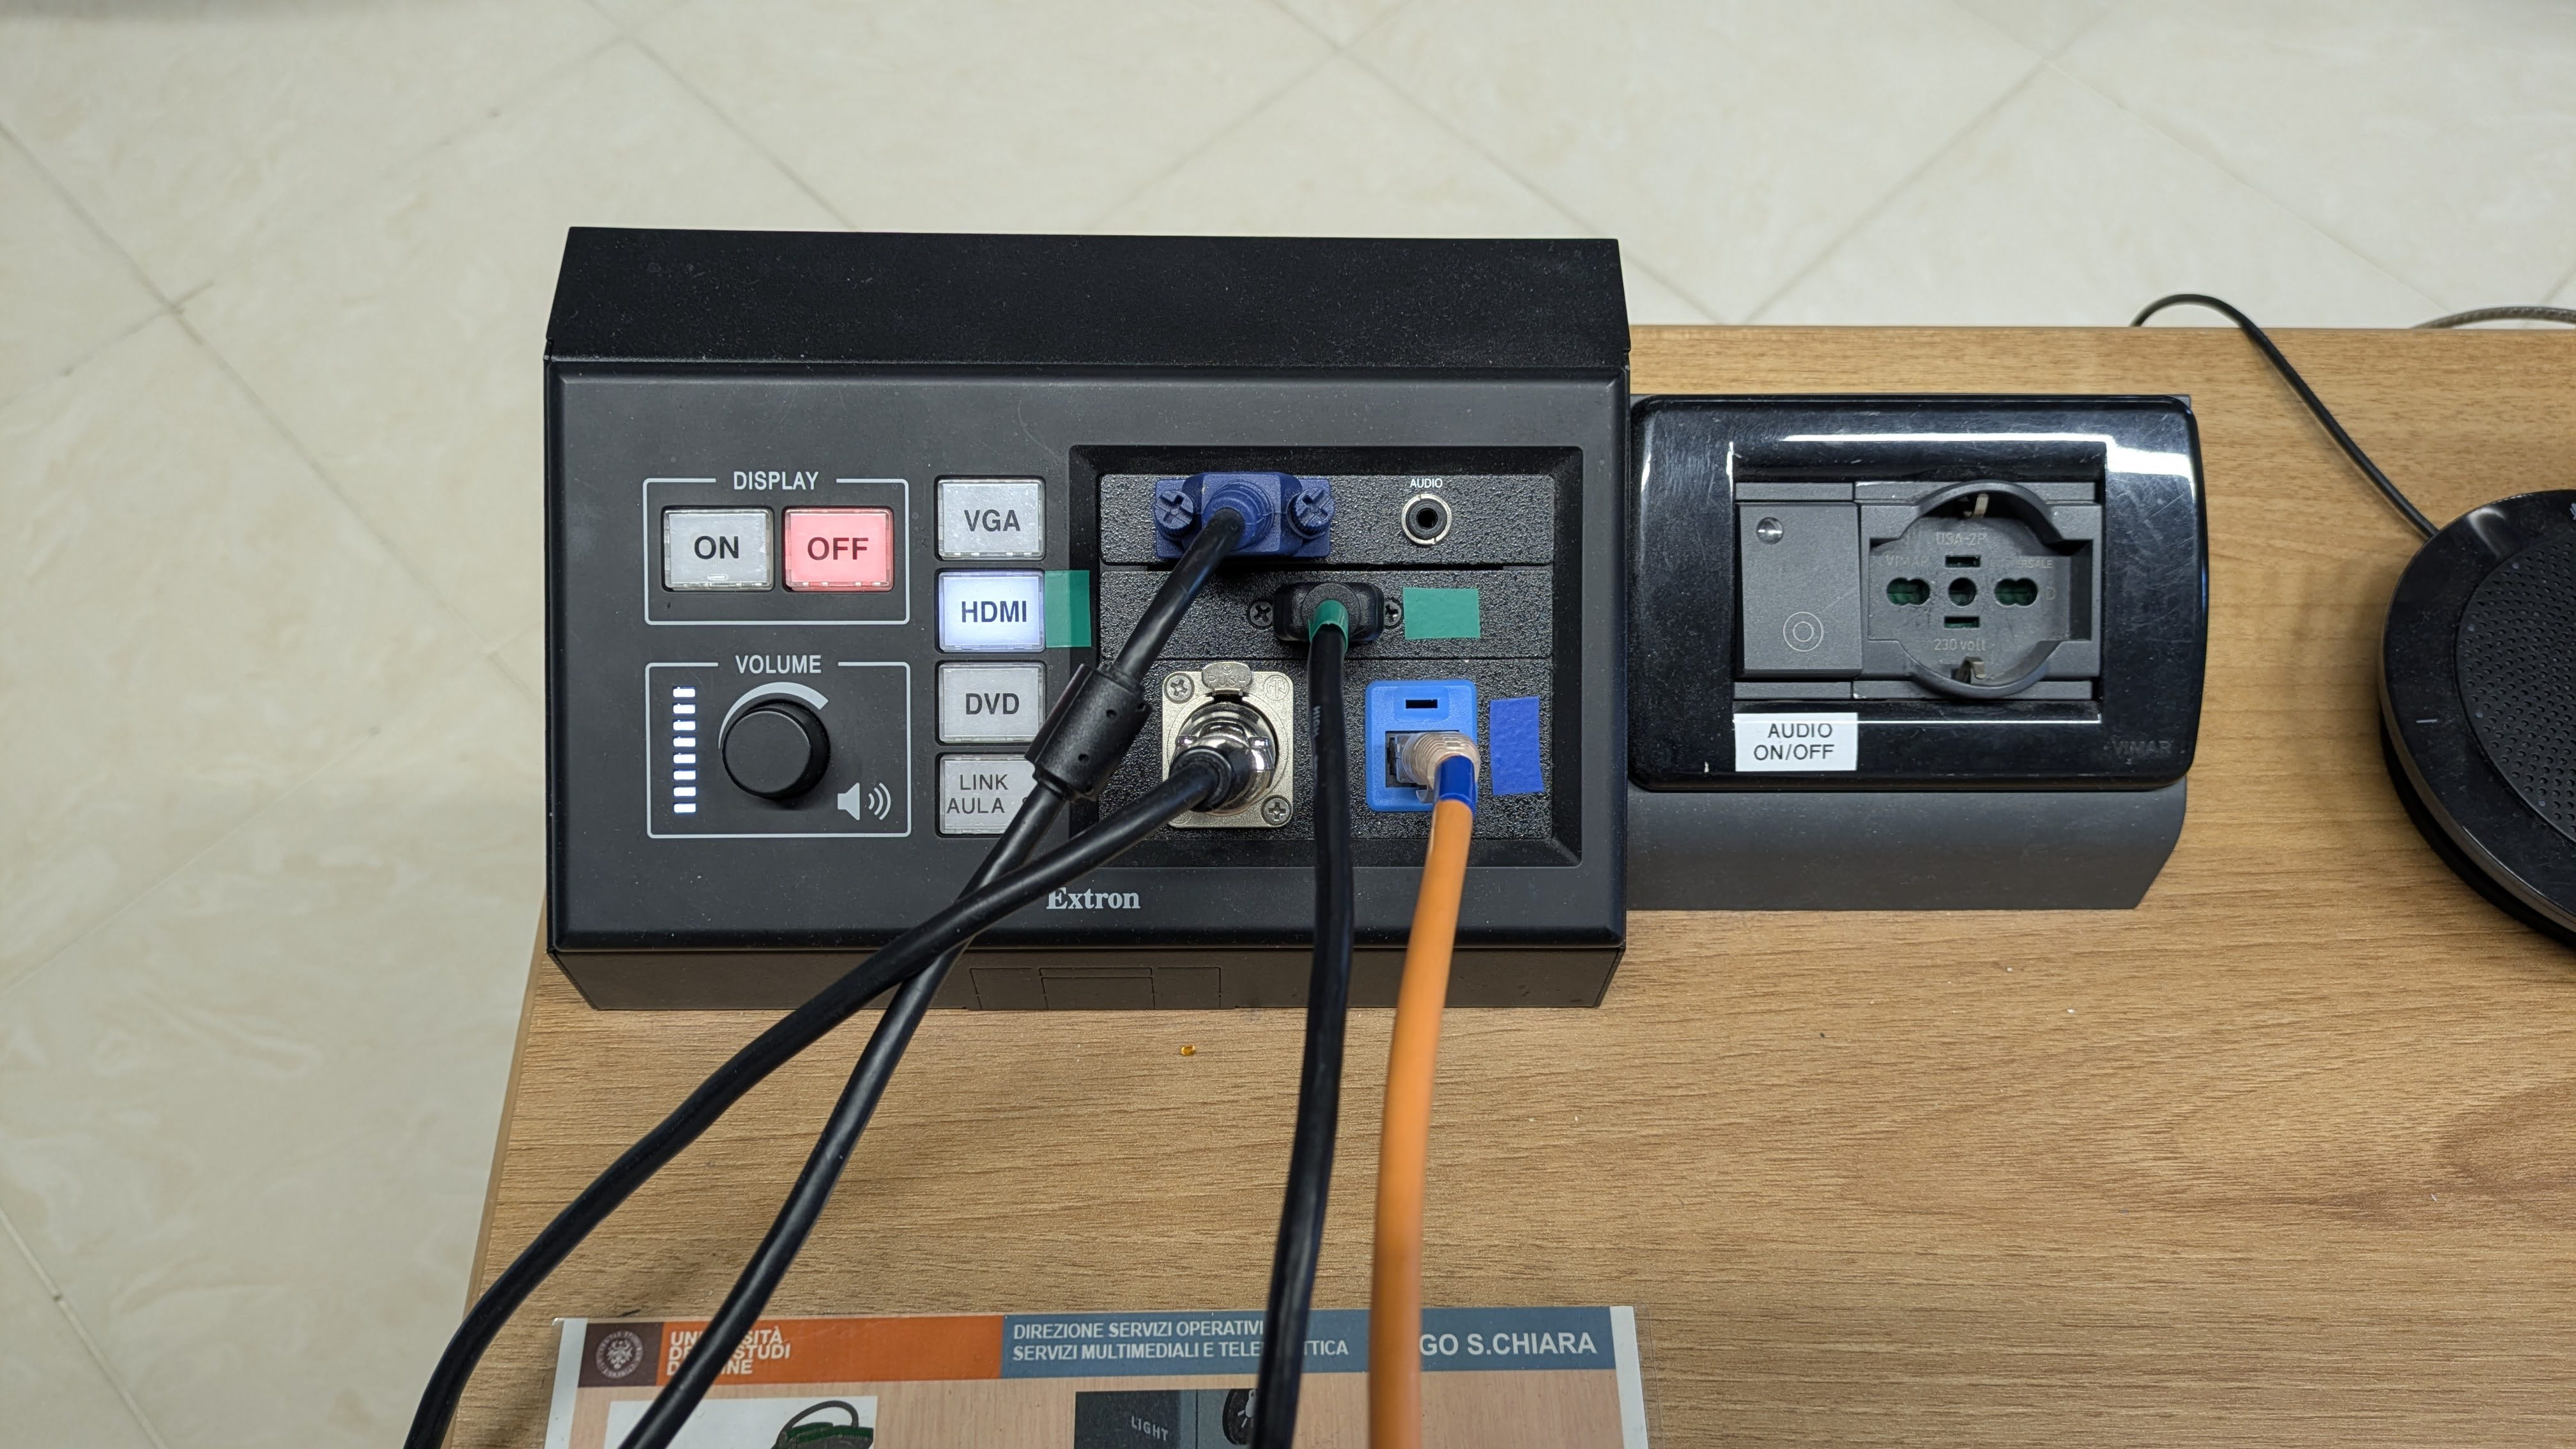
\includegraphics[width=12cm]{imgs/ControllerExtron.jpg}
                \caption{\textit{Controller Multimediale Extron}}
                \label{fig:extron}
            \end{figure}

            \hfill
            \begin{figure}[htbp]
                \centering
                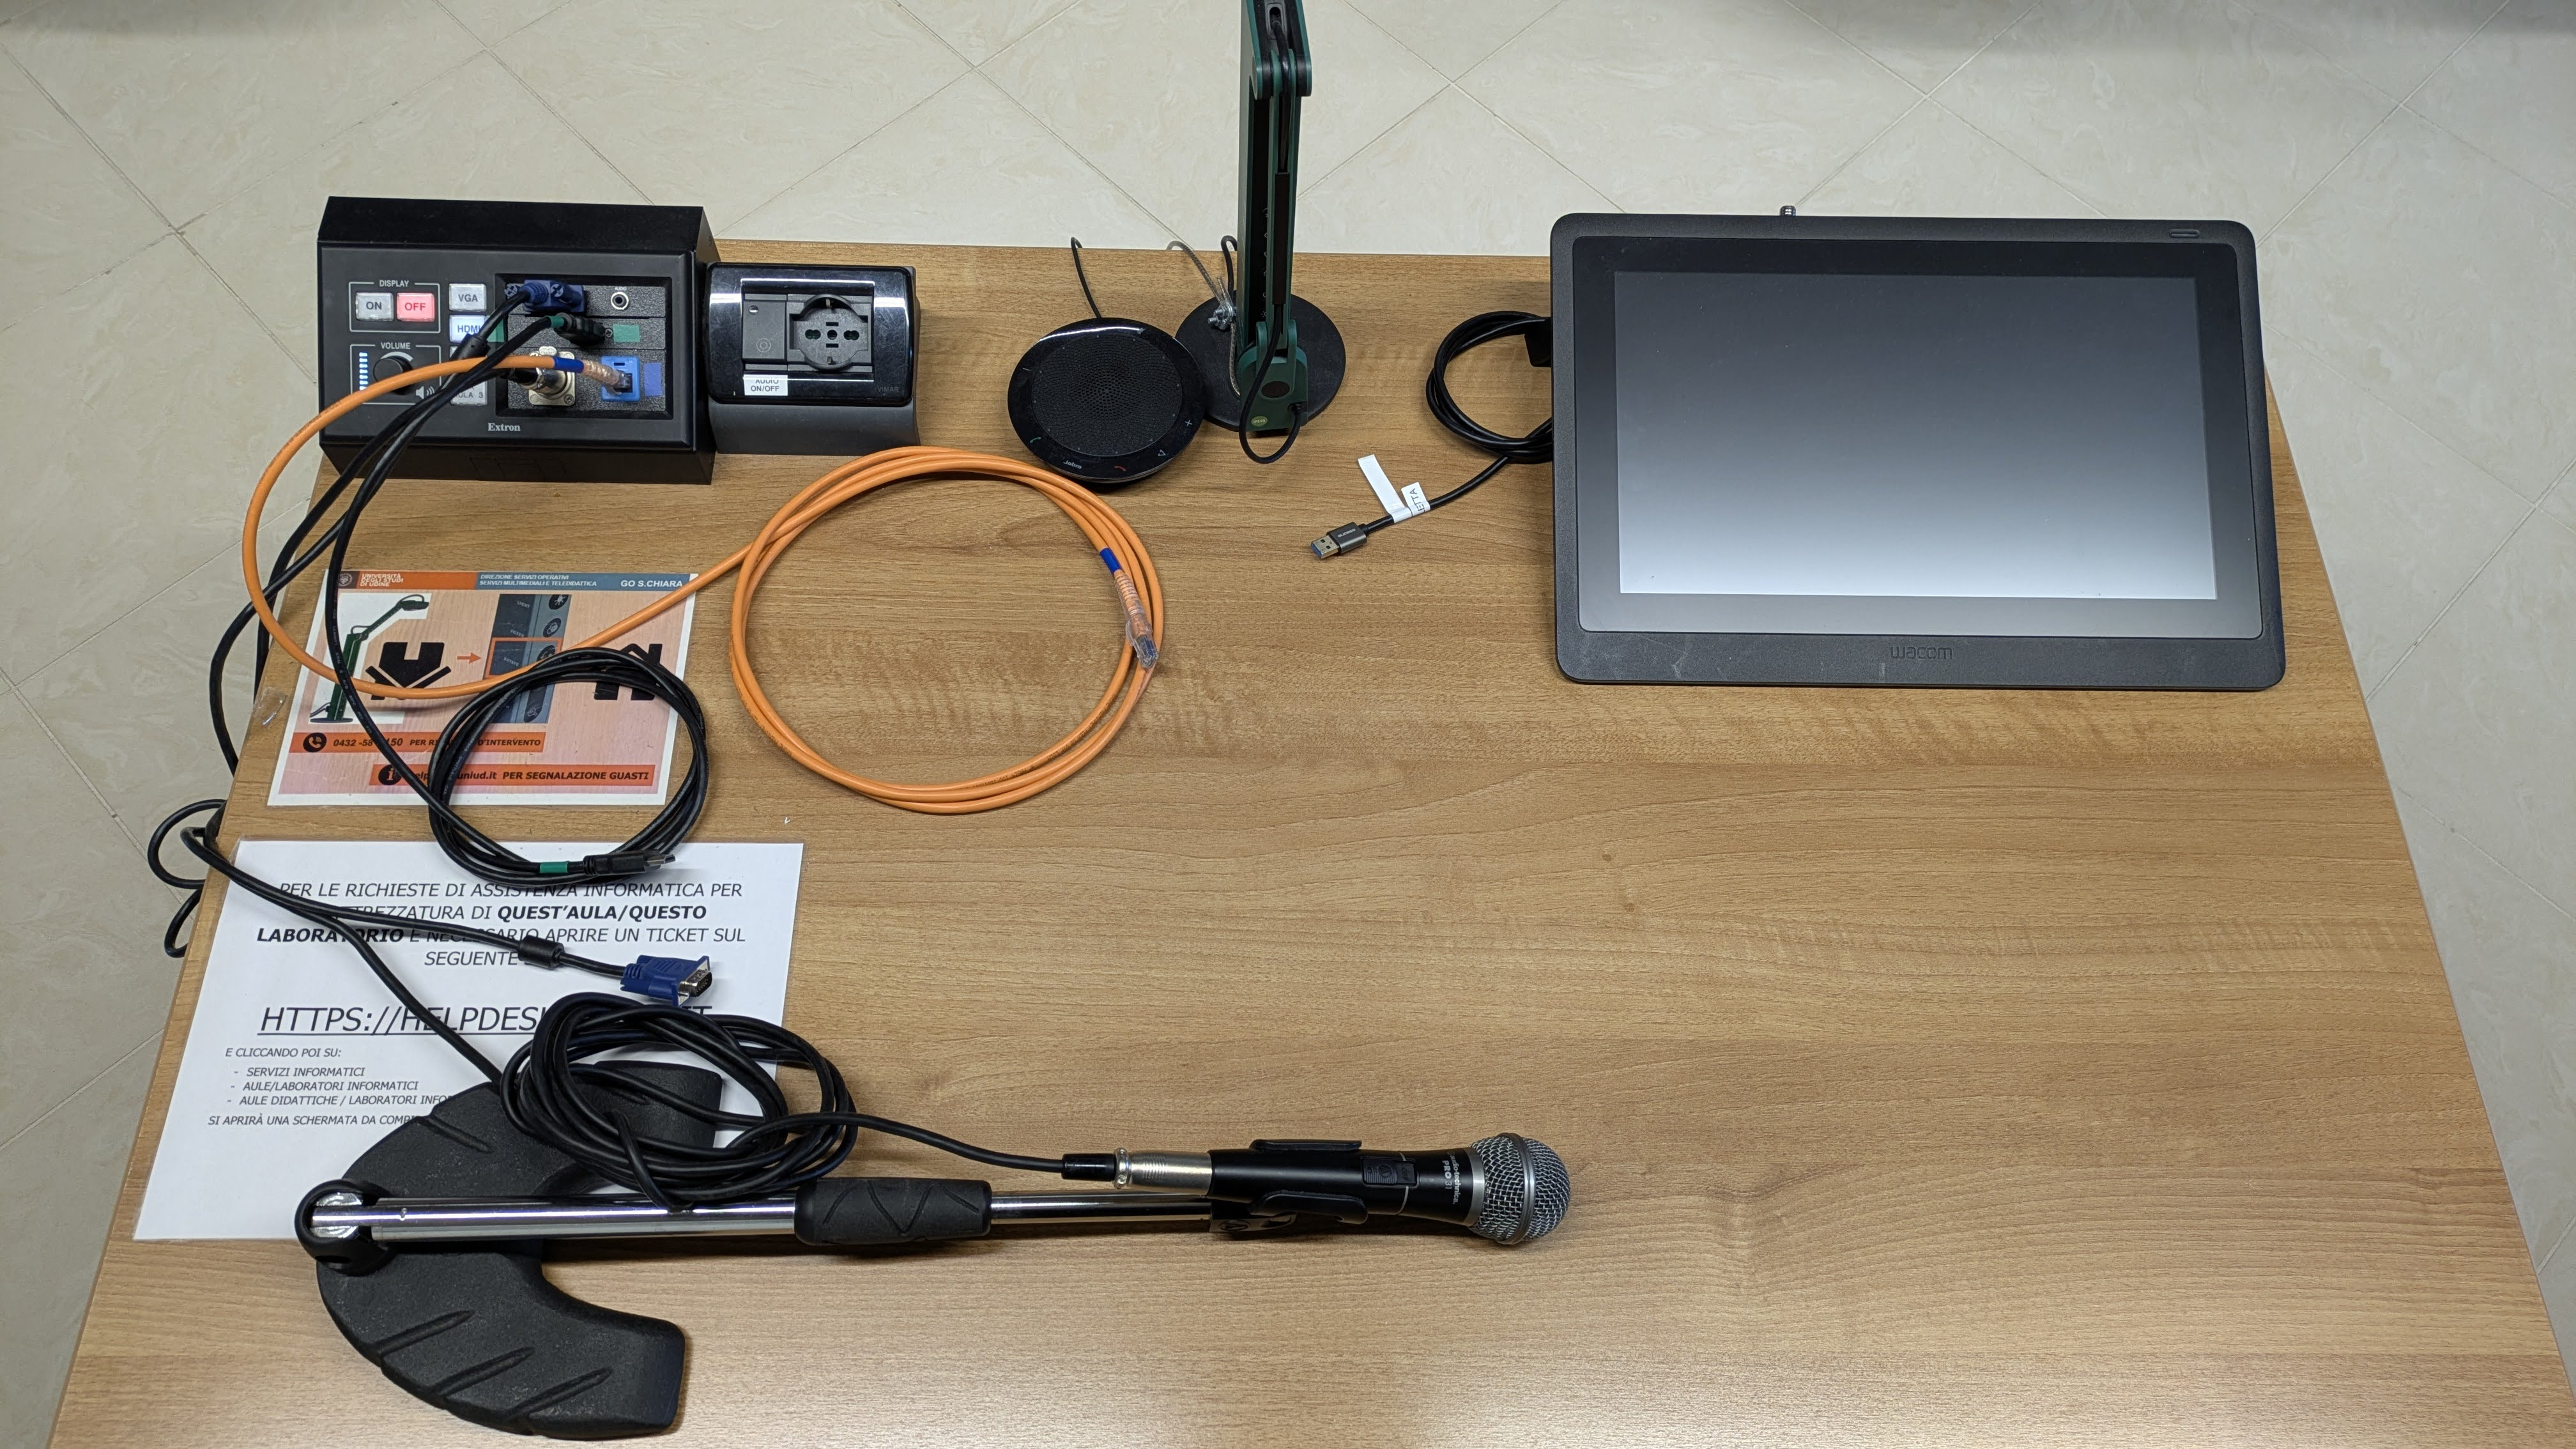
\includegraphics[width=12cm]{imgs/PostazioneDocente.jpg}
                \caption{\textit{Postazione docente delle aule multimediali}}
                \label{fig:postazioneDocente}
            \end{figure}
% ---------------------------------------------------------------------------------------
    \newpage
        \subsubsection{Collegamento Tipo all'impianto Multimediale}
            \par
                Nella seguente procedura non è contemplata la tipologia del computer preso in carico da parte del Docente, in quanto il sistema operativo di riferimento non influisce sulla qualità del servizio multimediale offerto. 
            \par
                L'accensione dell'impianto avviene tramite il tasto "ON" presente nel pannello frontale del controller e tramite la tecnica PoE accende il proiettore. Per il collegamento alla sorgente video, l'Università preferisce l'uso di cavi HDMI rispetto ai cavi VGA in quanto offrono una maggiore compatibilità e un'unica soluzione che comprende audio e video; entrambi però permettono di trasmettere in alta definizione in modalità progressiva (1080p)\footnote{\cite{HDMI22Specification}; "Le principali periferiche", "La gestione delle periferiche", \cite{sciutoIntroduzioneAiSistemi2022}}. 
            \par
                Per eseguire l'accesso ad Internet e poter navigare liberamente, sono necessarie le proprie credenziali Istituzionali. Il sistema distingue il login per studenti (\emph{spes.uniud.it}) da quello del personale interno e dei Docenti (\emph{uniud.it}). \newline
                La pagina di re-indirizzamento al login è basata sul protocollo HTTP, in quanto ha il solo scopo di presentare la prima richiesta alla pagina finale. Una volta che questa comunicazione avviene in qualche istante, bisogna inserite le credenziali e, indipendentemente dalla tipologia di utente autenticato, la comunicazione avviene solamente tramite il protocollo HTTPS in modo da poter trasmettere i vari messaggi in maniera sicura e crittografata attraverso la rete tramite i protocolli \textit{Secure Socket Layer} (SSL) oppure \textit{Transport Layer Security} (TLS). Entrambe le tecniche di crittografia sono valide per il protocollo HTTPS ma non sono interscambiabili (\textit{Figura 3.3}). Sia SSL che TLS permettono e garantiscono diverse proprietà che rendono sicuro il protocollo HTTP, queste sono: 
                \begin{itemize}
                    \item Negoziazione dei parametri: computer e server concordano quali algoritmi crittografici utilizzare.
                    \item Autenticazione del server: Il browser verifica l'identità del sito web tramite un certificato digitale.
                    \item Comunicazione segreta (Riservatezza): I dati vengono cifrati in modo che solo le due parti possano leggerli.
                    \item Protezione dell'integrità: Viene garantito che i dati non vengano manomessi durante il trasporto. 
                \end{itemize}
                Il computer avvia la comunicazione tramite un metodo \textit{handshake} che permette lo scambio delle chiavi crittografiche asimmetriche e, successivamente, la generazione delle chiavi utili alla creazione delle chiavi simmetriche\footnote{"Sicurezza del livello trasporto", \cite{tanenbaumRetiDiCalcolatori2011}}. \newline

            \begin{figure}[htbp]
                \centering
                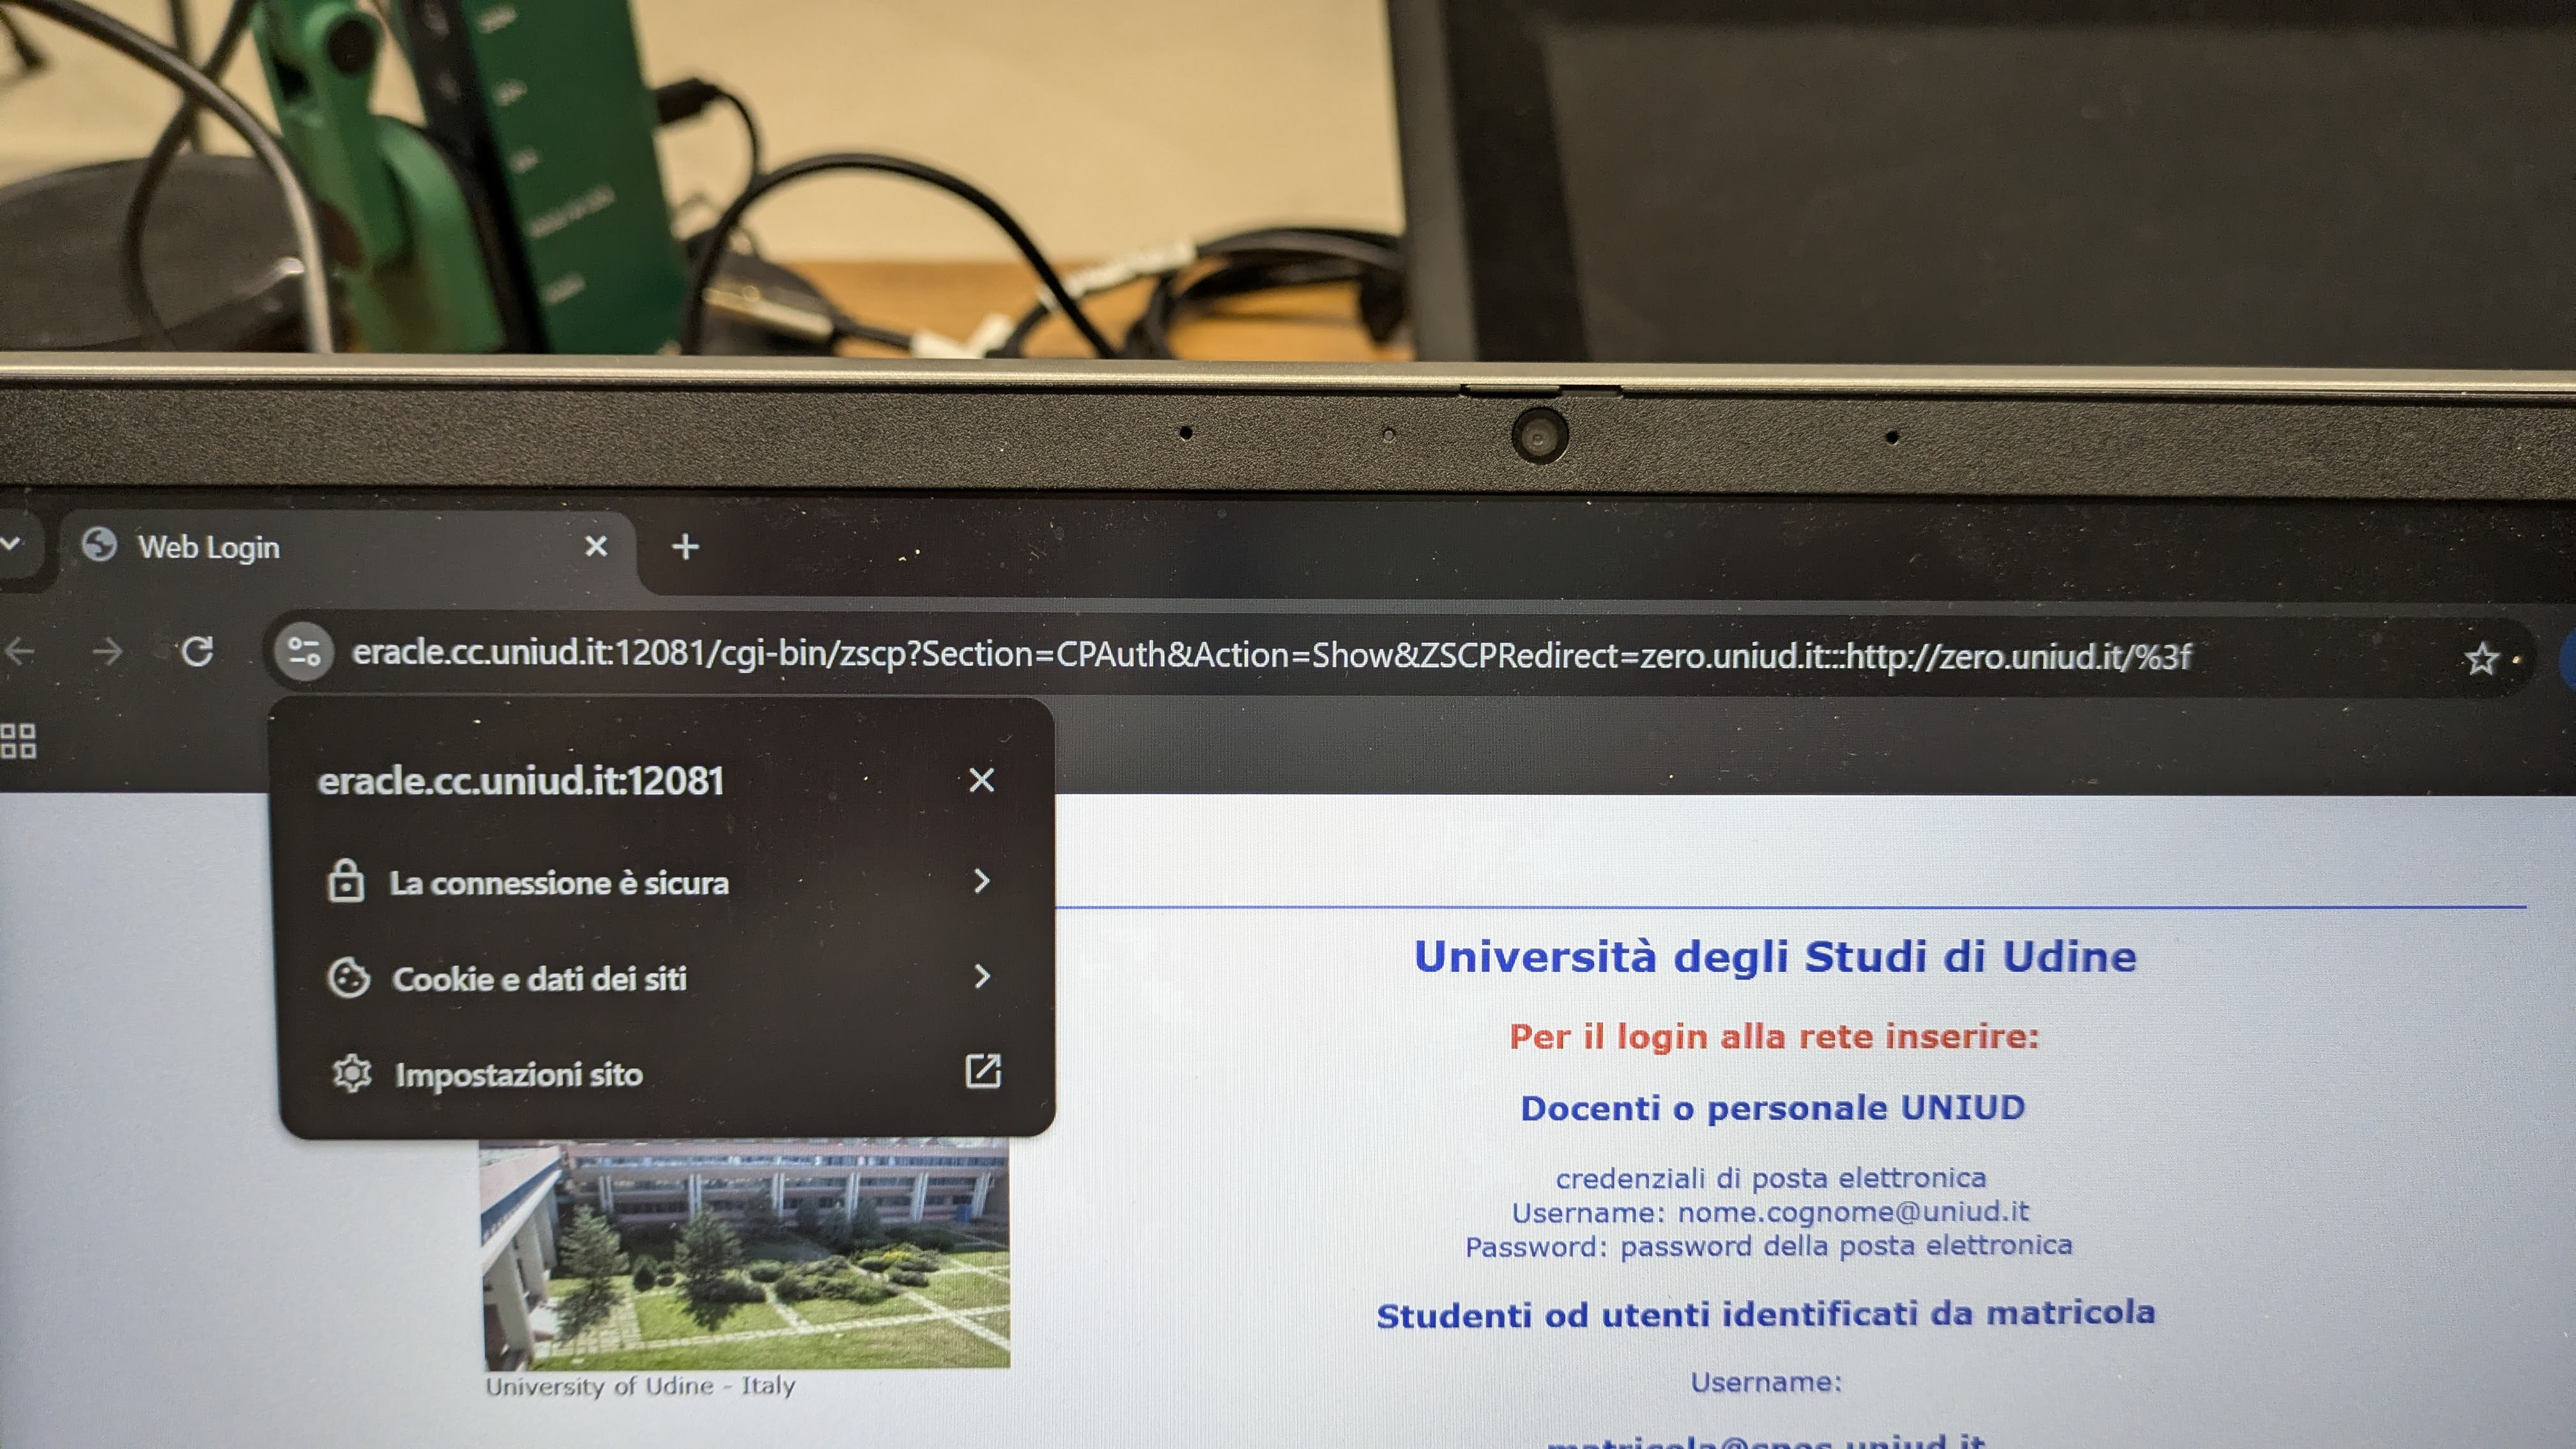
\includegraphics[width=12cm]{imgs/zeroshell.jpg}
                \caption{\textit{Pagina di Login a \emph{zero.uniud.it}}}
                \label{fig:zeroshell}
            \end{figure}

            \par
                Solamente dopo il login con le proprie credenziali si ottiene l'accesso ad Internet per un periodo di tempo determinato; la sessione ha durata diversa in base alla tipologia di account collegato. 
            \par
                L'accesso alla rete Internet non è fondamentale per l'avvio del proiettore tramite il controller \emph{Extron}; su questo controller è possibile trovare diversi tasti che ne regolano il funzionamento, permettendo il comando di altri dispositivi presenti e collegati all'impianto audiovisivo: 
                \begin{itemize}
                    \item Casse stereo; 
                    \item Amplificatore;
                    \item Microfoni direzionali.
                \end{itemize}
                Come descritto in precedenza, il controller Extron presenta un encoder digitale rotativo che permette il controllo preciso del volume in uscita dalle casse stero in dotazione alle aule. Inoltre, solitamente, presenta tre pulsanti dedicati alla gestione delle uscite video e audio ad esso collegate: due uscite HDMI e un'uscita VGA con jack audio da 3.5 mm. Le uscite audiovideo sono reciprocamente esclusive in quanto è impossibile mostrare una sorgente video che non sia stata selezionata dal pannello di controllo. Mentre il proiettore arriva a temperatura e inizia a funzionare, si abbassa il telo bianco dove poi si andrà a proiettare la sorgente video.
            \par
                Nelle aule sono presenti anche dei microfoni direzionali \textsl{gooseneck} o \textsl{cono gelato}; alcuni di questi sono wireless, altri sono cablati. Questi microfoni hanno al loro interno un tasto per poter bloccare la registrazione audio; per ridondanza il controller multimediale presenta un pulsante toggle "audio on/off" o "mute" che non solo blocca la registrazione da parte dei microfoni ma anche la riproduzione audio dalle casse stereo presenti in aula, "spegnendo" completamente il volume fino al prossimo click o alla chiusura dell'impianto (\textit{Figura 3.1}). 
            \par
                Il controller qui riportato è il dispositivo più comune presente nelle aule, tuttavia è presente una sua controparte touchscreen presso l'aula dell'Auditorium Fogar ma il funzionamento è pressoché identico, la sola differenza è la mancanza di un'interfaccia fisica. 
            \par
                Va posta particolare attenzione all'accensione dell'impianto stesso in quanto nella maggior parte dei casi esso viene acceso all'apertura del Centro Polifunzionale; nel caso tuttavia non fosse così, ogni aula ha a disposizione un interruttore che ne controlla accensione e spegnimento. Alcune di queste aule presentano anche un interruttore che, se tenuto premuto, abbassa manualmente il telo del proiettore (\textit{Figura 3.4}); entrambi gli interruttori sono etichettati per distinguerli dalle luci al neon a soffitto. 
                \newline

                \begin{figure}[htbp]
                    \centering
                    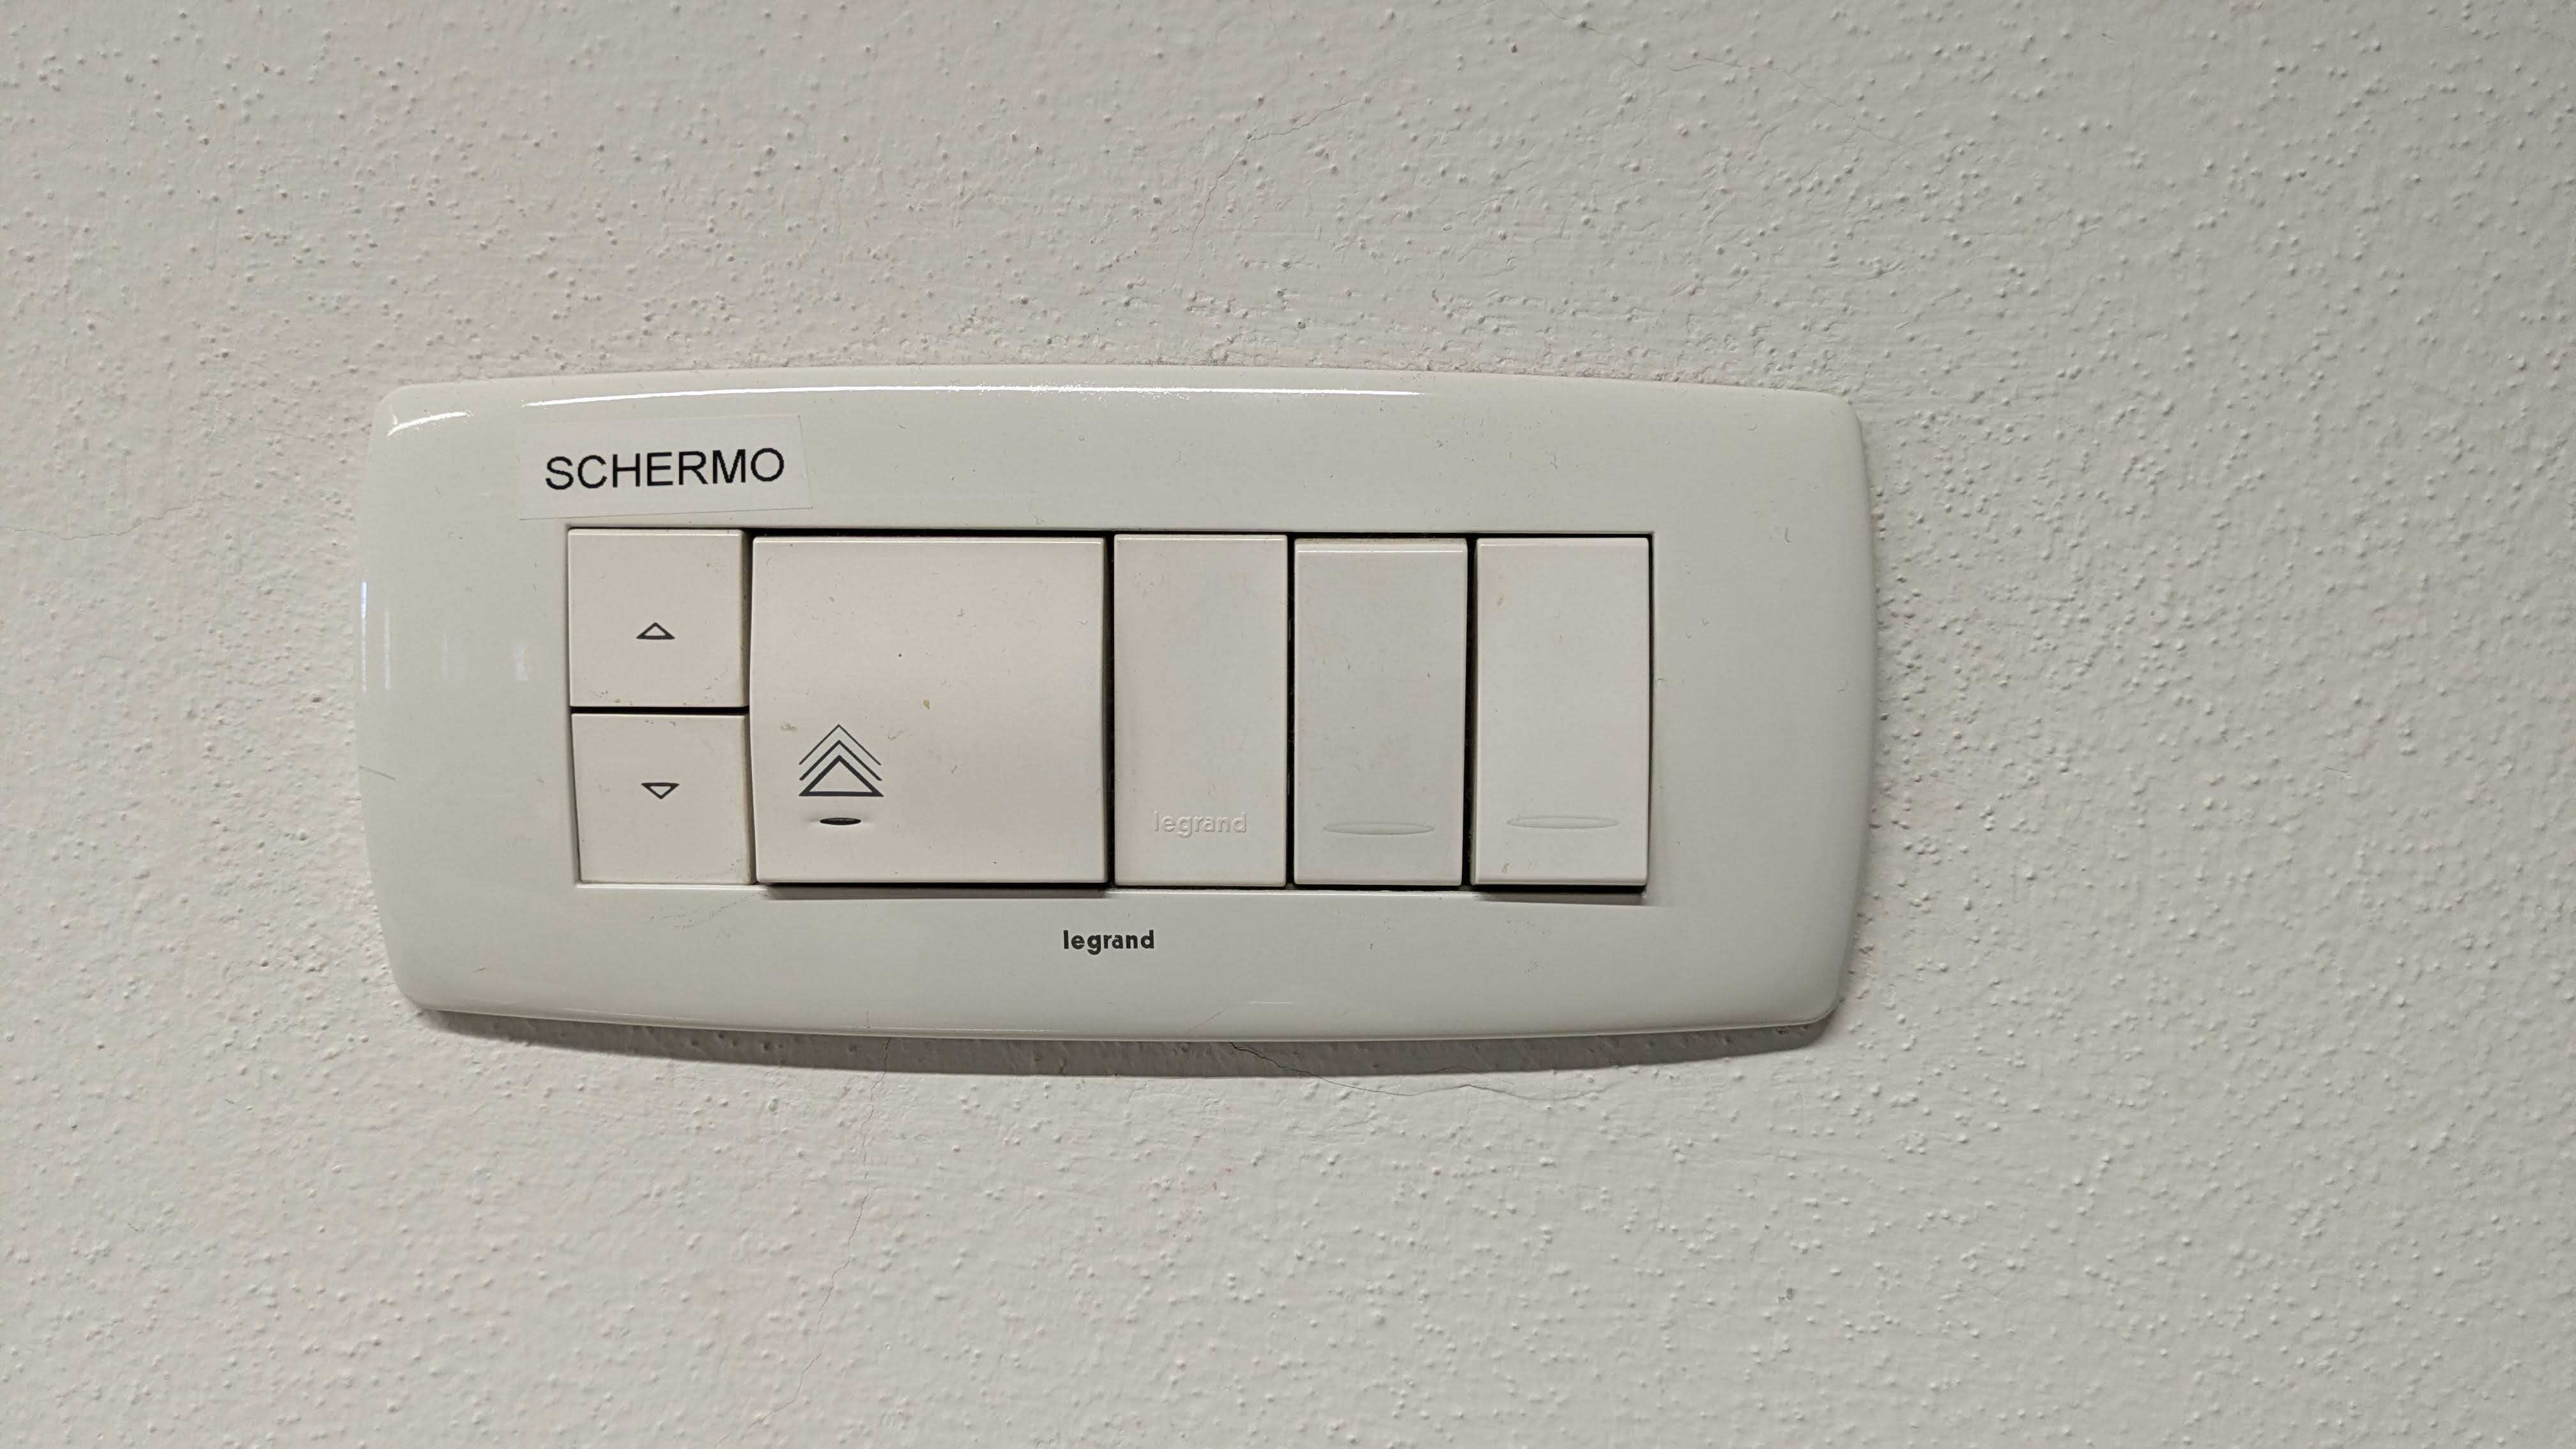
\includegraphics[width=12cm]{imgs/InterruttoriProiettore.jpg}
                    \caption{\textit{Interruttore per il controllo luci e proiettore}}
                    \label{fig:lightswitch}
                \end{figure}
                
            \par
                Il CEGO presenta anche un locale tecnico denominato "Centro Stella" dove si concentrano tutti i servizi TIC offerti dal server della Direzione e il router principale, nonché il collegamento alla backbone o dorsale che permette di interfacciarsi alla Rete di Ateneo. \newline
                All'interno del Centro Stella si possono trovare un server con diversi protocolli e servizi disponibili e un  \textit{Network Attached Storage} (NAS) per l'archiviazione di file e documenti, disponibile e accessibile in rete. 
            \par
                Il server presente all'intero del Centro Stella è stato configurato sulla base della distribuzione Linux Zeroshell. 
                Questa distribuzione è fortemente centrata sulle tecniche di routing e di bridging tra reti, permettendo una connessione completa senza soluzioni di continuità, pur mantenendo un notevole livello di sicurezza. \newline
                Tra i molteplici servizi che offre questa distribuzione Linux possiamo trovare: 
                \begin{itemize}
                    \item il servizio FTP: servizio dedicato allo scambio di file in modo da potervi accedere da qualsiasi postazione della Direzione, si interfaccia con il dispositivo NAS;
                    \item il servizio di Captive Portal: servizio che cattura tutto il traffico di rete e lo reindirizza ad una pagina  di autenticazione;
                    \item il servizio di Autenticazione RADIUS (\textit{Remote Authentication Dial-In User Service}): servizio che gestisce le credenziali di accesso degli utenti \emph{spes.uniud.it} e \emph{uniud.it};
                    \item il servizio Kerberos: servizio che permette l'autenticazione \textit{single sing-on} senza mai far trasmettere la password dell'utente in chiaro attraverso la rete;
                    \item il servizio Certification Authority: servizio che premette la validazione di certificati e firme digitali secondo lo standard X.509 v3, standard utilizzato per la trasmissione delle chiavi pubbliche;
                    \item il servizio Firewall: servizio mirato alla sicurezza filtrando l'accesso alla rete di virus e utenti malevoli;
                    \item il servizio di VPN: servizio che permette di configurare una rete privata virtuale, sia \textit{Host-to-LAN} che \textit{LAN-to-LAN};
                    \item il servizio VLAN Mapping: servizio che supporta lo standard IEEE 802.1Q, ovvero la creazione di più VLAN su specifici; 
                    \item il servizio QoS: servizio ormai presente su qualsiasi dispositivo di rete moderno, permette di bilanciare diversamente le varie tipologie di traffico di rete per garantire la migliore qualità di trasmissione. 
                \end{itemize}
                Il servizio FTP è un servizio progettato per permettere lo scambio di file e dati tra due o più computer o tra un computer e un server, creando una sorta di tunnel virtuale per l'\textit{upload} e successivo \textit{download} del file. In aggiunta a \textit{Zeroshell} si possono configurare funzioni aggiuntive di filtraggio e di monitoraggio degli accessi, ottimizzandone il recapito\footnote{"QoS and Traffic Shaping", \cite{ZeroshellLinuxRouter2021}}.
            \par
                Il servizio di Captive Portal funge da "rete di cattura" per tutto il traffico Internet, reindirizzando tutte le richieste ad una pagina di autenticazione, impostata dal pannello di controllo del server, in modo da accreditare ogni utente connesso. Le credenziali vengono controllate dal Captive Portal tramite il server RADIUS/Kerberos.
                \footnote{"Hotspot using Captive Portal", \cite{ZeroshellLinuxRouter2021}}
            \par
                Il servizio di autenticazione RADIUS permette una centralizzazione dell'autenticazione in un unico server, semplificando e alleggerendo il lavoro dei vari punti di accesso ospitando il database, o parte di esso, delle credenziali di accesso. Il servizio è stato idealizzato per reti cablate ma è utilizzato anche per le connessioni wireless\footnote{"Wireless e reti mobili", "Sicurezza nelle reti", \cite{kuroseRetiDiCalcolatori2022}} come può esserlo la rete di Ateneo \textit{Eduroam}.
            \par
                Il servizio di autenticazione Kerberos premette di autenticarsi in rete, come RADIUS, solamente con una tecnica diversa in quanto necessita di tre entità per poter creare una comunicazione sicura: l'\textit{Authentication Server} (AS), il \textit{Ticket-Granting Server} (TGS) e il server a cui si vuole accedere. Questa architettura permette l'inserimento della propria password solamente una singola volta e questa non verrà mai trasmessa in chiaro sulla rete. Entrando nei dettagli tecnici, questo protocollo lavora sugli orologi di sistema dei dispositivi, richiedendo che questi siano sincronizzati a quello del TGS. Il messaggio cifrato contenente i vari dati per la configurazione della comunicazione sicura è costruito attorno al messaggio che manda il TGS e quindi non è facilmente intercettabile da utenti terzi. Grazie a questa caratteristica architettonica del protocollo, è possibile scalare i servizi disponibili, predisponendo diversi reami con più AS, TGS e servizi a cui si vuole accedere\footnote{"Autenticazione con Kerberos", \cite{tanenbaumRetiDiCalcolatori2011}; "LDAP directories" \cite{ZeroshellLinuxRouter2021}}. 
            \par
                Il servizio di Certification Authority (CA) permette di autenticare in modo sicuro l'utente connesso e, soprattutto, ne garantisce l'univocità tramite la creazione di un certificato di sicurezza contenente la rispettiva chiave pubblica. Questi certificati sono firmati digitalmente da un algoritmo, scelto durante la fase di configurazione, e possono essere rinnovati o revocati. Per poter confermare un utente sconosciuto, il suo certificati viaggia per una catena di diverse CA fino alla Root CA, nel caso dell'Università di Udine è ipotizzabile che la Root CA si trovi all'interno della sede centrale d'Ateneo. \newline
                La conferma dei certificati di sicurezza è fondamentale per poter garantire una comunicazione sicura, sono omessi ma presenti nei dati tecnici di molti algoritmi sicuri tra cui SSL, TLS e le VPN\footnote{"Authentication on Wireless networks with 802.1x, WPA and WPA2", "Virtual Private Network (VPN)", "Virtual Private Network (VPN)", \cite{ZeroshellLinuxRouter2021}}. 
            \par
                Il servizio Firewall è fondamentale se si vuole proteggere la rete interna all'Università da attacchi malevoli mirati all'interruzione di servizio. Il firewall filtra tutto il traffico in entrata e in uscita dalla rete LAN in base a delle regole precedentemente configurate. Zeroshell integra anche un sistema di protezione dagli attacchi \textit{Denial of Service} (DoS)\footnote{"Firewall SPI and Packet Filter", \cite{ZeroshellLinuxRouter2021}}.
            \par
                Il servizio VPN permette di aggiungere flessibilità all'accesso di rete, permettendo di collegarsi alla rete LAN anche se non si è presenti fisicamente al suo interno. Questa connessione è creata tramite una rete virtuale privata, garantendo l'accesso autenticato al dispositivo inserito\footnote{"Virtual Private Network (VPN)", \cite{ZeroshellLinuxRouter2021}}. Questa tecnica è utilizzata per poter accedere da remoto al server NAS con i portatili in uso dalla Direzione. 
            \par
                Il servizio VLAN Mapping permette di far corrispondere reti VLAN a specifici identificativi di reti wireless in modo da gestire permessi e livelli di sicurezza diversi in base alle esigenze delle VLAN. È possibile creare un'assegnazione dinamica interfacciandosi con il servizio RADIUS oppure mappare manualmente le varie reti inserendo bridge virtuali che contrassegneranno il traffico come se fosse diretto a quella rete\footnote{"Wireless Access Point with Multiple SSID and VLAN Mapping", \cite{ZeroshellLinuxRouter2021}}. 
            \par
                Il servizio QoS ha un'architettura simile al servizio di firewall, in quanto filtra e monitora tutto il traffico che attraversa la rete. Questo monitoraggio è svolto con l'obiettivo di garantire i giusti pesi ai vari pacchetti che transitano in rete, per esempio offrendo una maggiore banda agli applicativi \textit{Voice-over-Internet-Protocol} (VoIP)\footnote{"QoS and Traffic Shaping", \cite{ZeroshellLinuxRouter2021}}. 
% ---------------------------------------------------------------------------------------
% revisione fino a qui --> in pausa fino a che non ho scritto molto
    \setcounter{chapter}{3}
\setcounter{section}{0}

\chapter{Mansioni}
        \par
            La seguente sezione illustra la suddivisione delle mansioni svolte durante il periodo del tirocinio curricolare. Generalmente si possono distinguere gli interventi di \textit{Collaborazione alla gestione Informatica e Multimediale}, gli interventi di \textit{Manutenzione degli Impianti Informatici e Audiovisivi di un Polo Universitario} e infine alcuni interventi di natura generale, non riconducibili alle due categorie sopra elencate. 
% ---------------------------------------------------------------------------------------
        \section{Collaborazione alla gestione Informatica e Multimediale}
            \par
                Gli interventi principali di Collaborazione alla Gestione Informatica riguardano gli aggiornamenti software dei vari computer comprendendo quelli in uso all'Amministrazione, quelli in uso alla Biblioteca, quelli presenti nei Laboratori di Informatica 1 e 2 e quelli in uso ai Docenti. Tutti questi computer operano sulla versione 25H2 di Windows Enterprise, permettendo una copertura da patch della sicurezza future. I due Laboratori di Informatica hanno una trentina di computer ciascuno e ognuno di questi è configurato per poter permettere l'accesso al proprio account tramite Server di Autenticazione RADIUS gestito dall'Università degli Studi di Udine. L'account di accesso ha le stesse credenziali del proprio account istituzionale (\emph{spes.uniud.it}). Una nota di apprezzamento va espressa nei confronti degli impianti di entrambi i laboratori: questi due operano sulla stessa VLAN in modo da poter permettere una comunicazione tra tutti i computer; i Laboratori inoltre presentano una telecamera che inquadra la postazione docente offrendo la possibilità di trasmettere il flusso video nell'altro laboratorio, tramite uno schermo dedicato.  \newline
                Ogni computer ha la possibilità di accedere con un account locale con privilegi di amministratore, ma questo viene utilizzato esclusivamente per l'installazione e la configurazione di software richiesto dal Corpo Docenti o per poter eseguire interventi di manutenzione straordinaria. 
            \par
                La collaborazione alla gestione informatica comprende anche il supporto informatico e multimediale per tutta la durata di eventi, di convegni e di symposium. Prima del loro inizio si verifica la stabilità dell'impianto e il corretto funzionamento dei microfoni e delle casse stereo, predisponendo poi due computer in modo da registrare audio e video dell'evento intero per fornirlo quindi agli studenti che ne richiedono l'accesso durante l'evento stesso in modo da fornire supporto immediato. Ad evento terminato si spegne l'impianto e si verifica lo stato della registrazione completa; non appena questa viene elaborata dai server di Teams, si prevede il caricamento sui canali ufficiali. \newline
                Nel caso i Relatori di un evento abbiano anticipato alla Direzione della necessità di un collegamento su Teams, si predispone la chiamata tra il Relatore o Relatrice connessi e i restanti presenti nell'aula, in modo che chi sia connesso possa seguire la durata dell'intero evento e intervenire al momento ritenuto opportuno. 
            \par
                Durante il primo semestre si sono svolti i Test d'Ingresso per il Corso di Laurea in Relazioni Pubbliche. Il compito svolto riguardava la predisposizione dei computer presenti nei due Laboratori di Informatica, avviandoli, accedendo ad un account dedicato e lanciando il software Safe Exam Browser (SEB) dato che i Test offrono una correzione automatica al loro termine. Mentre gli studenti eseguivano i test, la presenza del sottoscritto è stata fondamentale in quanto ne fornisce supporto immediato ai problemi che si sono verificati. \newline
                Durante una sessione dei Test d'Ingresso, ho segnalato a chi di competenza due computer desktop che hanno avuto problemi. Rispettivamente un computer aveva problemi di natura hardware in quanto non riscontrava alcun segnale video nonostante il monitor fosse collegato al computer, mentre l'altro dispositivo aveva problemi di natura software, in quanto SEB mostrava una finestra di dialogo con un errore riferito alla mancata presenza del file di configurazione.
% --------------------------------------------------------------------------------------       
            \subsection{Configurazione Tablet}
                La Prof.ssa Pocecco, referente del Dipartimento di Lingue e Letterature, Comunicazione, Formazione e Società (DILL), ha acquistato una decina di tablet Samsung Galaxy Tab A7 destinati a progetti proposti a studenti. Questi tablet, acquistabili solo da aziende ed enti certificati, sono ottimi per una connessione On-The-Go (OTG) a riunioni online, fornendo un ottimo e accessibile supporto informatico e digitale. \newline
                Solamente alcuni dispositivi erano stati configurati in precedenza all'avvio del Tirocinio e mi sono occupato quindi di inizializzarli tramite il processo di setup iniziale di Android e, una volta terminato, di predisporli completamente all'uso. \newline
                Per poterli configurare in maniera il più possibile simile al login dei computer dei Laboratori di Informatica 1 e 2 ho dapprima disinstallato tutte le app di servizi terzi non utili ai fini dei vari tablet, del tipo Netflix, Amazon e altre applicazioni simili; successivamente ho limitato l'uso di altre applicazioni disabilitandone il servizio, quale per esempio l'accesso a Gmail. Infine ho suggerito alla Direzione di creare un account Google necessario per poter  installare l'applicazione \textsl{Boot Apps}, la quale permette l'avvio automatico di qualsiasi applicazione e servizio, installando e optando per l'avvio automatico della sola app \textsl{Geteduroam}. Ho deciso di seguire questa configurazione dato che il sistema operativo Android 10 OneUI 2.5 non permette l'avvio automatico di app a meno che non siano di sistema. \textsl{Geteduroam} così facendo, si trasforma in una sorta di setup guidato che permette la configurazione e successiva connessione alla rete \textsl{Eduroam}; l'app necessita di una prima connessione ad Internet per potersi connettere al server RADIUS disponibile all'interno dell'Università. Una volta che ci si è accreditati tramite il proprio utente istituzionale, la connessione Internet precedente non è più essenziale. \newline
                Un'ulteriore serie di applicazioni installate sono legate alla suite di Microsoft, comprendendo Word, Excel e Teams. \newline
                Data l'amplia base di utenti a cui saranno destinati i tablet e la distribuzione che deve essere prima concessa dalla Prof.ssa Pocecco, si è deciso di non inserire alcuna password d'accesso in modo da poterli utilizzare con facilità. Tutt'ora questi dispositivi sono utilizzati durante le riunioni della Direzione per prendere appunti e per seguire collegamenti su Teams. 
% -------------------------------------------------------------------------------------- 
            \subsection{Gestione degli eventi}
                \par
                    Come descritto in precedenza, il supporto informatico e multimediale è esteso anche alla gestione degli eventi. Questo supporto, oltre a coprire la durata degli eventi stessi, si traduce nel tenere aggiornato il calendario degli eventi stessi, per poi comunicarlo a chi di competenza. Questa scaletta era prima mantenuta in un foglio di calcolo Excel condiviso contenete una tabella con i campi più importanti quali titolo, data, ora, descrizione; per poter aggiornare il file, bisognava modificare i permessi di condivisione; dato che esso era di proprietà di un ex collega, si è optato per la creazione di un altro file, basato sul foglio di calcolo condiviso, in modo da poter archiviare il precedente, ormai obsoleto. \newline
                    Dopo una riunione con alcuni rappresentati della Direzione del CEGO, si è deciso di migrare questo file alla piattaforma online Microsoft Planner, creando diversi contenitori dove si inserivano le varie attività e gli eventi da poter poi aggiornare "in corso d'opera".
                \par 
                    Microsoft Planner ha permesso alla Direzione di avere una maggiore visione d'insieme per quanto riguarda tutte quelle tipologie di eventi e di compiti assegnati ai vari membri del personale. Nello specifico uno di questi contenitori riguardava gli interventi programmati di manutenzione informatica e una parte di formazione del personale, approfondita in seguito. 
                    L'intervento programmato più pressante riguardava l'aggiornamento e la riconfigurazione di rete dei vari dispositivi mobili, quali i portatili per i Docenti, i tablet e i portatili della Direzione, con le nuove impostazioni di sicurezza della rete \textsl{Eduroam}. \newline
                    L'aggiornamento è avvenuto senza problemi per i tablet, in quanto non richiedevano alcuna credenziale di amministratore; per i portatili della Direzione invece è stato richiesto l'intervento del Dott. Castelli per poter lanciare l'eseguibile di configurazione con permessi superiori. Infine, per quanto riguarda i portatili in dotazione ai Docenti, si è deciso di non aggiornare alle nuove impostazioni di sicurezza in quanto essi sono principalmente collegati ad Internet tramite connessione cablata, garantita dall'Università e presente in ogni aula e Studio Docenti. 
% --------------------------------------------------------------------------------------
            \subsection{Gestione dei CFU soprannumerari degli Studenti}
                 \par
                    In relazione alla gestione degli eventi, ognuno di questi rilasciava agli studenti partecipanti un attestato soprannumerario con valenza di 0,25 CFU, 0,50 CFU o più raramente 0,75 CFU. Per tenerne traccia la Segreteria studentesca del CEGO ha utilizzato un foglio di calcolo Excel. Questo file era stato concepito per la semplice catalogazione e l'aggiornamento di ogni singola carriera degli studenti in modo da fornire un calcolo dei CFU soprannumerari a fine carriera. Il compito assegnatomi riguardava la semplificazione del file precedente per renderlo più accessibile, mantenendo i dati già inseriti e prevedendo l'aggiunta dei vari certificati futuri. \newline
                    Il file è una sorta di database delle carriere studentesche composto da quattro tabelle di cui una è pivot: la prima tabella contiene i dati anagrafici degli studenti (matricola, cognome, nome, corso); la seconda tabella contiene nome e data degli eventi, estrapolati dal file di organizzazione precedentemente citato, e il valore del certificato dell'evento; la terza tabella mette in relazione gli studenti con gli eventi cui hanno partecipato con l'inserimento di sola matricola e nome dell'evento seguito; l'ultima tabella è di tipo pivot ed è risultante dalla relazione precedente, fornendo la somma dei CFU ottenuti dai vari corsi associata ai dati dello studente o studentessa. \newline
                    Logicamente, queste tabelle operano come un database la cui relazione tra i dati degli studenti e gli eventi si traduce in una relazione uno a molti\footnote{"Il sottosistema GD", \cite{sciutoIntroduzioneAiSistemi2022}}, ovvero che uno studente, con matricola univoca, può e ha seguito almeno un evento e quindi, nella tabella degli eventi seguiti, la sua matricola comparirà più di una volta. \newline
                    Si è deciso di mantenere l'organizzazione del calcolo dei CFU soprannumerari in un file Excel in quanto offre un'accessibilità maggiore a tutto il personale, senza dover installare e mantenere un server SQL o Access all'interno del server presente nel Centro Stella.
% ---------------------------------------------------------------------------------------
            \subsection{Formazione del personale in merito agli Impianti Informatici e Multimediali}
                    Come citato in precedenza, mi sono occupato anche di formare il personale, distinguendo la formazione in due gruppi differenti, create sulla base dell'obiettivo e il target: la prima categoria comprende i Tutor e i nuovi tirocinanti mentre la seconda comprende il personale esterno della Portineria. 
                \par
                    Per quanto riguarda i Tutor e i nuovi tirocinanti, la formazione ha incluso una parte di illustrazione di collegamento agli impianti e una carrellata di problemi che si possono verificare, come per esempio la mancanza del segnale video sul proiettore. Inoltre ho fornito supporto alla condivisione e alla produzione di grafiche basate anche sulla nuova identità visiva dell'Università, installando il font \textsl{Work Sans} e impostandolo come predefinito per i nuovi modelli dell'identità visiva. \newline
                    L'obiettivo di questa formazione è stato rendere i Tutor più autonomi in caso di assenza del Tecnico durante gli eventi; invece l'obiettivo fissato per i nuovi tirocinanti riguardava più il passaggio di consegne, anche in previsione della fine del mio tirocinio curricolare. 
                \par
                    Per quanto riguarda il personale esterno della Portineria, bisogna sottolineare un primo passaggio di richiesta alla Direzione, la quale ha avuto esito positivo dopo essersi messa in contatto con l'ente esterno Sicuritalia. La formazione, simile a quella per i Tutor e per i nuovi tirocinanti, riguardava per lo più gli impianti: come funzionano sinteticamente e cosa fare in caso di problemi tecnici facilmente risolvibili, soprattutto in relazione al segnale audio e al segnale video. \newline
                    L'obiettivo invece di questa formazione era rendere più efficace l'intervento del Tecnico in caso di problemi gravi agli impianti informatici e multimediali, dato che la maggior parte dei Docenti si interfaccia dapprima con il personale di turno della Portineria che a loro volta contatteranno il Tecnico.
                \par
                    La formazione, indipendentemente dal target e l'obiettivo, è stata basata sul documento "DAGS Formazione Personale 2025" fornitomi dalla Direzione in previsione della fine del mio tirocinio curricolare. 
% ---------------------------------------------------------------------------------------
        \section{Manutenzione degli Impianti Informatici e Audiovisivi di un Polo Universitario}
            \par
                Uno dei compiti assegnatomi è stato quello di mantenere gli impianti informatici e audiovisivi del CEGO in uno stato ad hoc; questo si è tradotto in più interventi mirati alla risoluzione dei problemi tecnici riguardanti tutte quelle problematiche relative al segnale audio e al segnale video, localizzandole alla sola postazione del docente o all'impianto presente nelle aule multimediali. \newline
                La maggior parte di questi interventi si sono svolti durante i primi minuti di ogni blocco ore di lezione, in quanto molto spesso i problemi tecnici si verificavano non appena i Docenti andavano a collegarsi all'impianto audiovisivo con il portatile appositamente a disposizione, oppure il loro computer personale. In questo ultimo caso, tutte le operazioni che sono andato ad eseguire le ho svolte con il Docente a fianco, mostrandogli e illustrandogli apertamente cosa fare, mantenendo il più alto livello di riservatezza e intervenendo solamente se necessario. \newline
                Nel corso del tirocinio, solamente pochi miei interventi hanno richiesto il supporto di un Tecnico Informatico in contratto con l'Ateneo e questi pochi interventi hanno richiesto solamente il reset o la riconfigurazione del controller o del proiettore o, nel peggiore dei casi, la sostituzione del commutatore. 
            \par
                Di seguito vengono elencati quattro interventi ordinati in base alla gravità e durata dell'intervento, oltre all'applicazione della teoria appresa durante il Corso di Studi.
% ---------------------------------------------------------------------------------------
            \subsubsection{Intervento sulla configurazione delle Stampanti}
                    Il primo intervento ha riguardato la configurazione e la predisposizione delle stampanti nuove assegnate ai Laboratori di Informatica 1 e 2. Le stampanti erano precedente installate nei laboratori ma mancavano ancora della configurazione lato software, soprattutto nei vari computer messi a disposizione degli studenti. \newline
                    Queste due stampanti, una per laboratorio, sono usate dagli utenti e quindi devono essere disponibili indipendentemente dalla postazione che decide di usare lo studente. La stampante, inoltre, è stata precedentemente configurata limitando le operazioni eseguibili tramite le impostazioni accessibili dal proprio monitor; questa scelta è stata fatta presumibilmente per questioni di sicurezza e organizzazione dell'impianto. \newline
                    Per poter configurare le stampanti all'interno dei vari computer, ho eseguito l'accesso su ogni computer con l'account utilizzato per i Test d'Ingresso e, su ogni macchina, ho avuto accesso alle impostazioni e ho aggiunto manualmente la stampante del rispettivo Laboratorio. Infine su ogni computer è stata impostata la stampante del proprio laboratorio come predefinita, semplificando ulteriormente il processo di stampa da parte degli studenti.
                \par
                    Le stampanti moderne, come quelle in uso nei Laboratori, offrono la possibilità di creare delle code di stampa virtuali tramite la tecnica dello spooling, tecnica fondamentale nel contesto multi-utente del Laboratorio. Questa tecnica introduce un programma intermediario tra il computer e la stampante, gestendo e organizzando la coda di stampa in modo da poter garantire il servizio ad ogni utente connesso. Onde evitare che ogni utente connesso alla stessa rete dei Laboratori potesse avere accesso alla stampante e quindi intercettasse o alterasse la coda di stampa, si è deciso di gestire gli accessi da una lista (Access Control List) che ne bloccasse l'accesso agli utenti non autorizzati\footnote{"La gestione delle periferiche", \cite{sciutoIntroduzioneAiSistemi2022}}.
% ---------------------------------------------------------------------------------------
    \newpage
            \subsubsection{Intervento sul proiettore in Auditorium Fogar}
                    Il secondo intervento ha riguardato un problema avvenuto al proiettore dell'Auditorium Fogar, presso il Polo di Corso Verdi. Questo proiettore, come ogni altro proiettore presente al CEGO, è collegato ad un controller multimediale presente sulla postazione del docente in aula e si accende comunicando con la tecnica PoE. \newline
                    Il proiettore, connesso sia al ricevitore del controller sia all'alimentazione, non riceveva alcun il segnale video nonostante ricevesse l'impulso di accessione. Dato che in settimana si sarebbe svolto l'evento "Welcome Day" per le matricole iscritte al A.A. 2025/2026 con le autorità del Comune di Gorizia presenti, era essenziale far sì che l'intero impianto multimediale funzionasse correttamente. Dopo un mio primo sopralluogo, in cui ho verificato la connessione di tutti i cavi presenti nella postazione docente, ho verificato poi con un altro dispositivo oltre al computer precedentemente connesso. Dopo più cicli d'avvio, su suggerimento della Direzione, si è deciso di aprire un ticket di assistenza urgente. \newline
                    L'intervento si è svolto nel corso della giornata successiva alla segnalazione del problema al Dott. Barreca con il quale mi sono interfacciato e ho fornito tutti i dettagli necessari affinché si potesse risolvere il problema all'impianto. Per poter meglio isolare l'origine di questo malfunzionamento, io e il Tecnico siamo saliti in regia, dove si trova il ricevitore del controller connesso al proiettore stesso; da qui ci siamo connessi direttamente al proiettore verificando il suo corretto funzionamento, isolando in una prima fase il problema alla comunicazione tra il controller e il suo ricevitore. Successivamente, dopo un ciclo di spegnimento e riaccensione, il proiettore si è "riagganciato" al segnale proveniente dal controller posizionato sulla postazione docente, tornando così alla sua configurazione precedente, risolvendo per tempo il malfunzionamento.
                    %
                \par
                    Per creare il canale di comunicazione tra controller e ricevitore, ma soprattutto per usare la tecnica PoE, è necessario che entrambi questi due dispositivi siano connessi da un cavo di rete Ethernet con rispettiva porta RJ45. Questo cavo è composto da più coppie di cavi, coordinati in base al colore, utilizzati per il collegamento ad Internet; esistono diverse categorie ordinate per velocità e frequenza crescenti, le più comuni sono 5e (Cat. 5 Enchaned), 6 e 7. Tutte queste tre categorie supportano velocità di trasmissione da 1 Gbps fino ai 10 Gbps della Cat. 7 però ne risentono della distanza, soprattutto se questa sfora i 100 metri. La differenza sostanziale tra queste tre categorie è la costruzione fisica del cavo in quanto i cavi di Cat. 5e sono tutti \textsl{Unshielded Twisted Pair} (UTP), i cavi di Cat. 6 sono sia UTP che \textsl{Shielded Twisted Pair} (STP) mentre i cavi di Cat. 7 sono \textsl{Shielded/Foiled Twisted Pair} ovvero che i cavi di Cat. 6 presentano una schermatura solamente attorno alla guaina protettiva più esterna mentre i cavi di Cat. 7 presentano sia una guaina protettiva esterna che una serie di altre guaine protettive intorno ad ogni coppia di doppini\footnote{"Le infrastrutture di rete", \cite{sciutoIntroduzioneAiSistemi2022}}. 
% ---------------------------------------------------------------------------------------
            \subsubsection{Intervento sulla tavoletta grafica in Auditorium Fogar}
                    Anche questo intervento ha riguardato l'Auditorium Fogar e la tavoletta grafica presente su ogni postazione docente del CEGO. La tavoletta è di norma collegata all'impianto tramite cavo HDMI e successivamente collegata al computer tramite cavo USB. Questa doppia connessione permette sia la duplicazione del monitor a cui è collegata sia l'uso dello \textsl{stylus} tramite la connessione USB; come ogni periferica, per poter garantire la più completa compatibilità bisogna installare i driver opportuni, già presenti nei computer dati in dotazione ai Docenti. \newline
                    La tavoletta era già stata precedentemente segnalata tramite il sistema di ticket dell'Università a causa di un apparente guasto al segnale video. Il giorno successivo alla segnalazione, mentre offrivo supporto all'evento "\textsl{Come scrivere una tesi di laurea degna di lode}" tenutosi presso il Polo di Santa Chiara, ho ricevuto una chiamata da parte del Dott. Barreca per poter verificare di persona la veridicità del guasto. \newline
                    Per isolare i vari componenti e quindi meglio identificare il problema che causava la mancanza di segnale video, ho portato un monitor avente anch'esso un'uscita HDMI. L'uso di questo monitor ausiliario ha permesso di circoscrivere il problema allo splitter HDMI (\textit{Figura 4.1}), utile in congiunzione con il controller multimediale, oppure alla tavoletta grafica. Lo splitter HDMI presenta, oltre alla porta di alimentazione, un'entrata HDMI dalla sorgente collegata e due uscite che duplicano tale entrata. \newline
                    Una volta collegato il monitor ausiliario all'alimentazione e all'uscita HDMI presente, ho potuto constatare che il problema poteva riguardare la tavoletta grafica piuttosto che lo splitter stesso; nell'andare a verificare il corretto funzionamento della tavoletta grafica e quindi scollegare il cavo utilizzato al monitor HDMI, ho notato che dallo splitter non vi era alcuna entrata da duplicare sulla tavoletta grafica e che il solo cavo collegato all'impianto del controller era quello presente sulla postazione docente, rendendo lo splitter effettivamente "inutile". \newline
                    Sulla postazione docente dell'Auditorium, il Docente può collegarsi su tre punti diversi, senza andare ad alterare l'impianto stesso: due collegamenti sono sulla postazione mentre l'ultimo è presente sul leggio. Date queste possibilità di collegamento, i cavi di ciascuna sono stati raggruppati in due guaine in maglia espandibile, una per la postazione e una per il leggio, in modo da poter semplificare i collegamenti e facilitare l'eventuale spostamento della postazione docente. Tuttavia ho dovuto ricablare la postazione docente, aggiungendo un cavo HDMI allo splitter, in modo da rendere la tavoletta funzionante, mantenendo intatto il segnale video diretto al proiettore; il cavo HDMI utilizzato era già presente, fissato sotto alla postazione docente con delle fascette adesive, presumibilmente proveniente da una configurazione precedente che contemplava una posizione diversa della tavoletta grafica. \newline
                    Per assicurarmi il funzionamento complessivo dell'impianto, ho eseguito l'intervento con una sorgente video sempre connessa e, ad ogni spostamento di cavo, ricontrollavo la qualità complessiva. Da aggiungere che durante il ricablaggio ho notato una forte interferenza proveniente dall'impianto audio; sono riuscito ad isolare il problema a uno dei microfoni presenti sulla postazione, immaginando un collegamento non corretto ma, una volta acceso singolarmente, l'interferenza persisteva; una volta accertato che il collegamento fosse corretto, ho notato un difetto alla base del microfono stesso che, al minimo movimento, produceva l'interferenza andando a macchiare la qualità audio. \newline
                    L'intervento si è concluso segnalando al Dott. Barreca il corretto funzionamento della tavoletta grafica e dell'impianto intero ma aggiungendo il guasto inatteso del microfono. Su suo suggerimento e grazie alla Direzione, il microfono guasto è stato spedito per posta interna agli uffici del DAGS ai fini di una tempestiva soluzione. 

                    \hfill
                \begin{figure}[htbp]
                    \centering
                    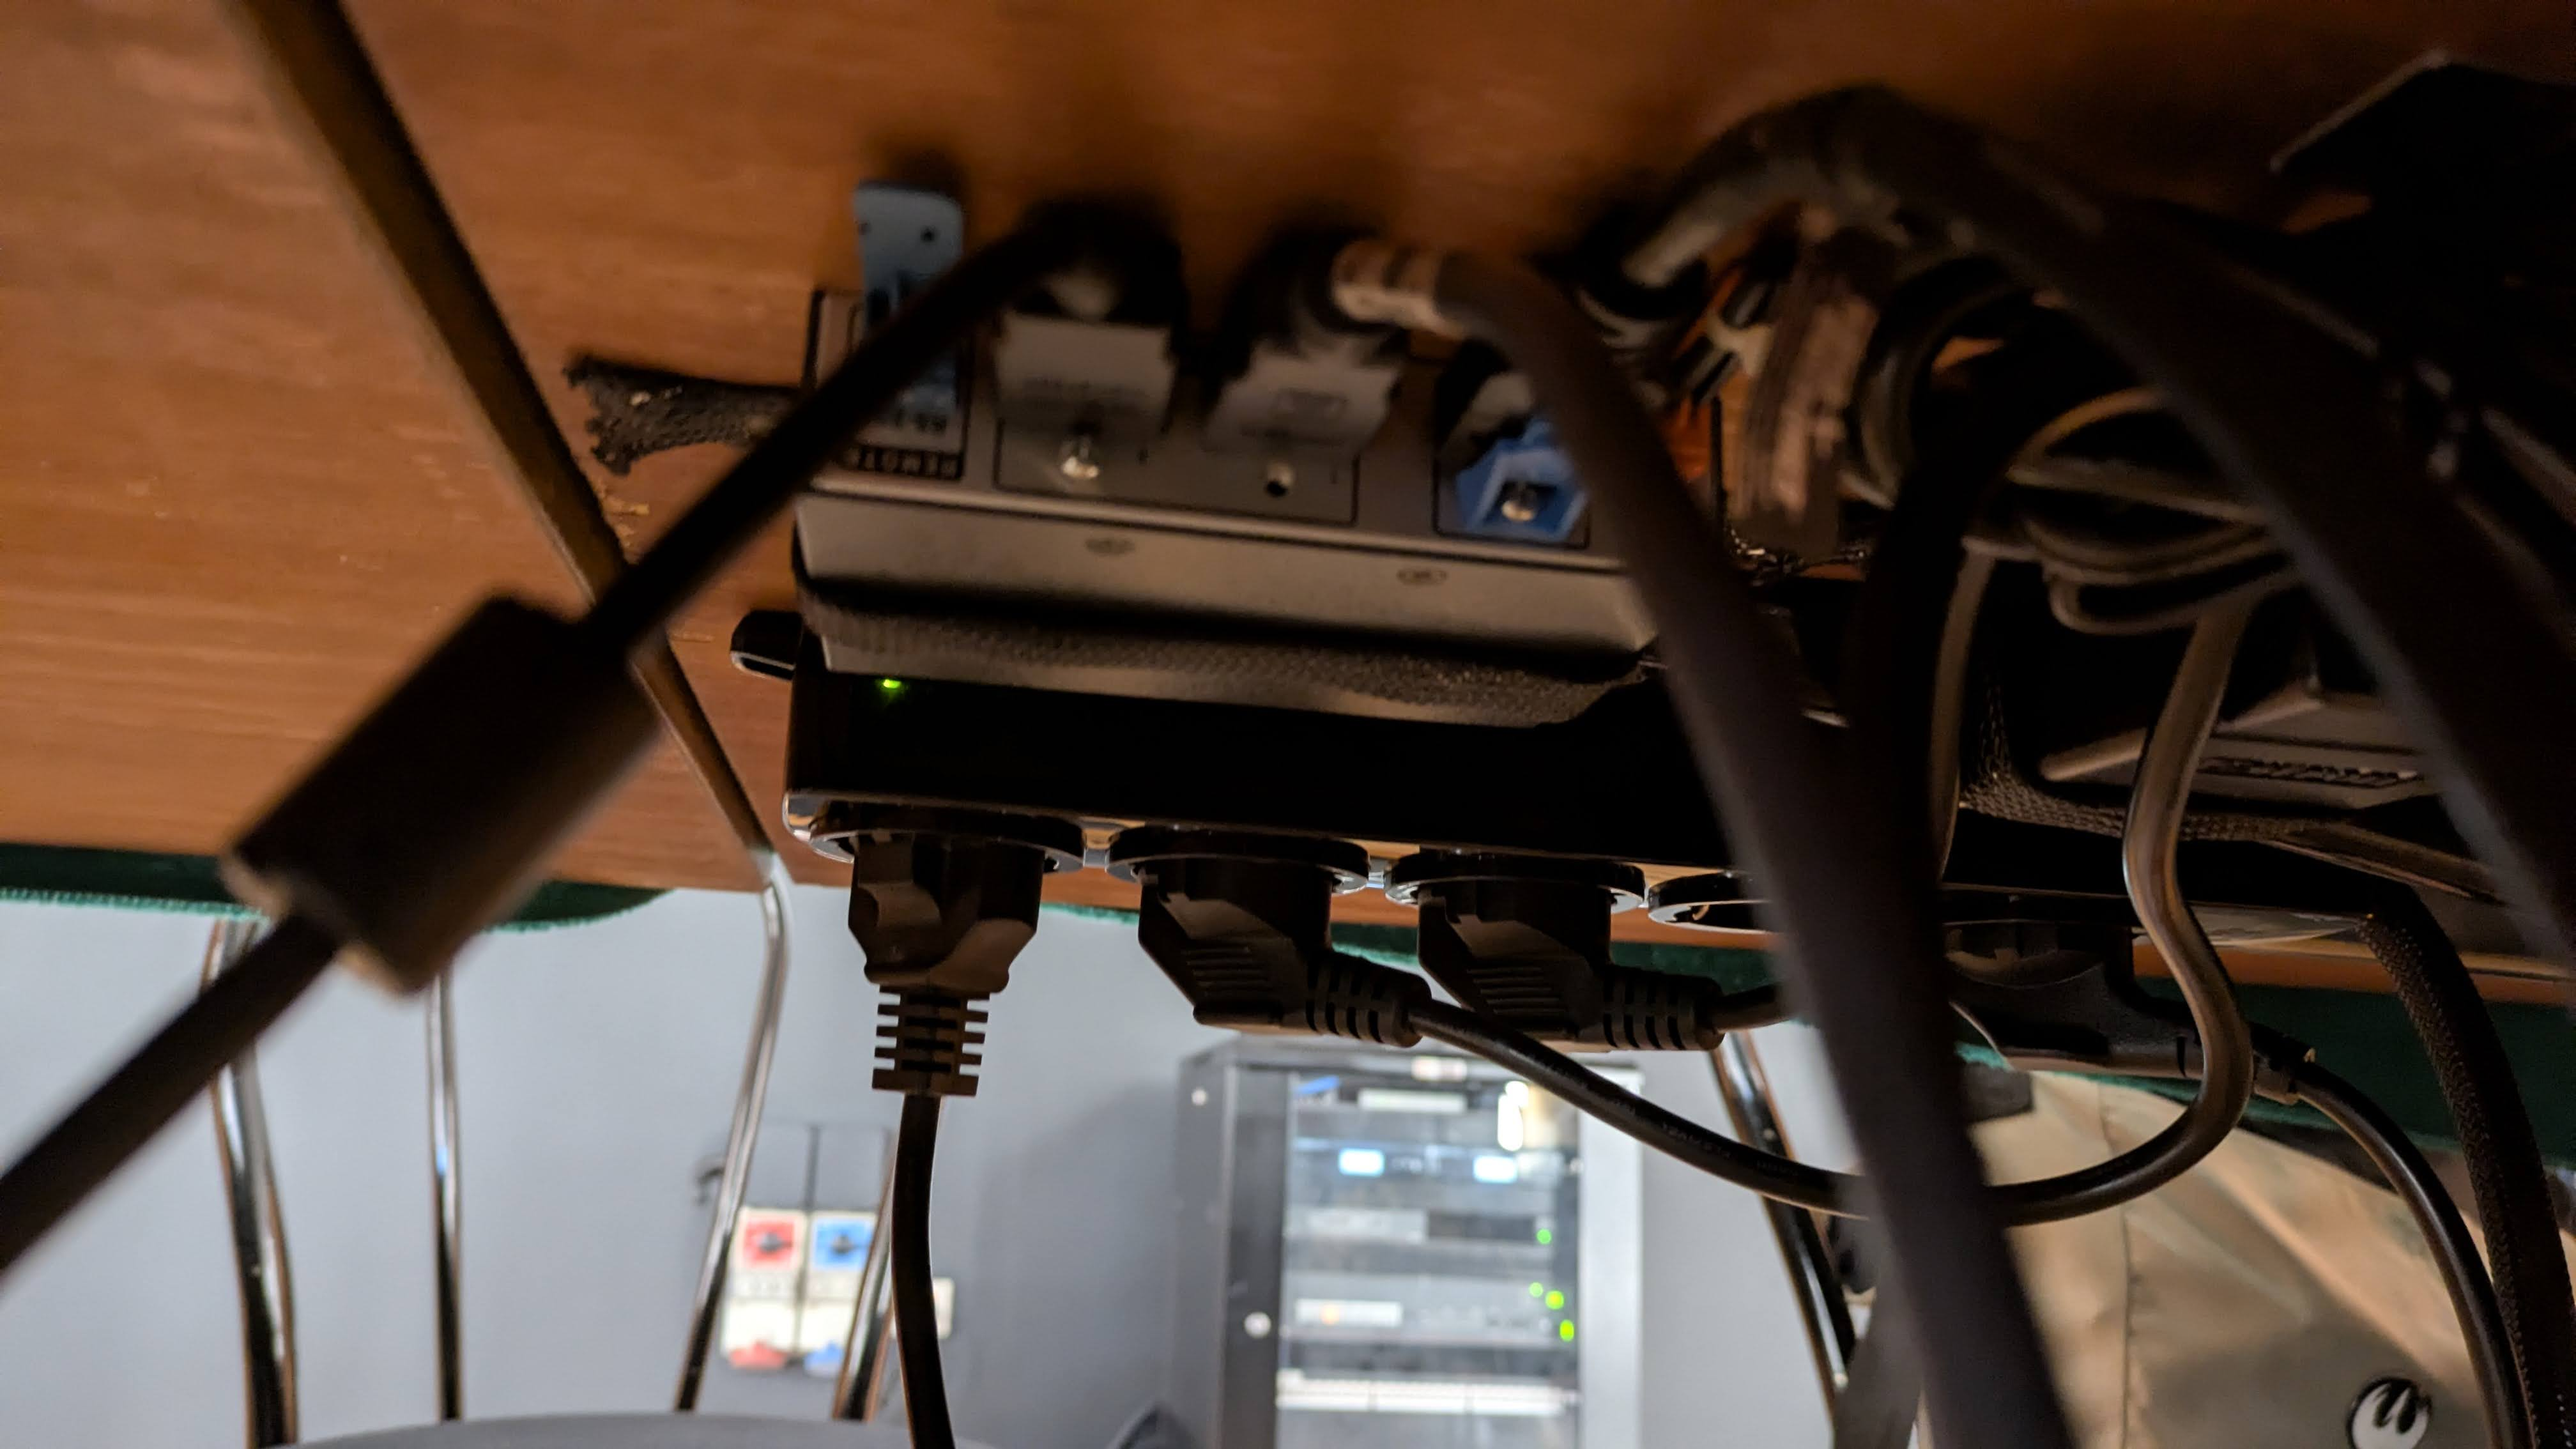
\includegraphics[width=12cm]{imgs/commutatore.jpg}
                    \caption{\textit{Splitter HDMI posto al di sotto della postazione docente}}
                    \label{fig:splitterWacom}
                \end{figure}
        
                \begin{figure}[htbp]
                    \centering
                    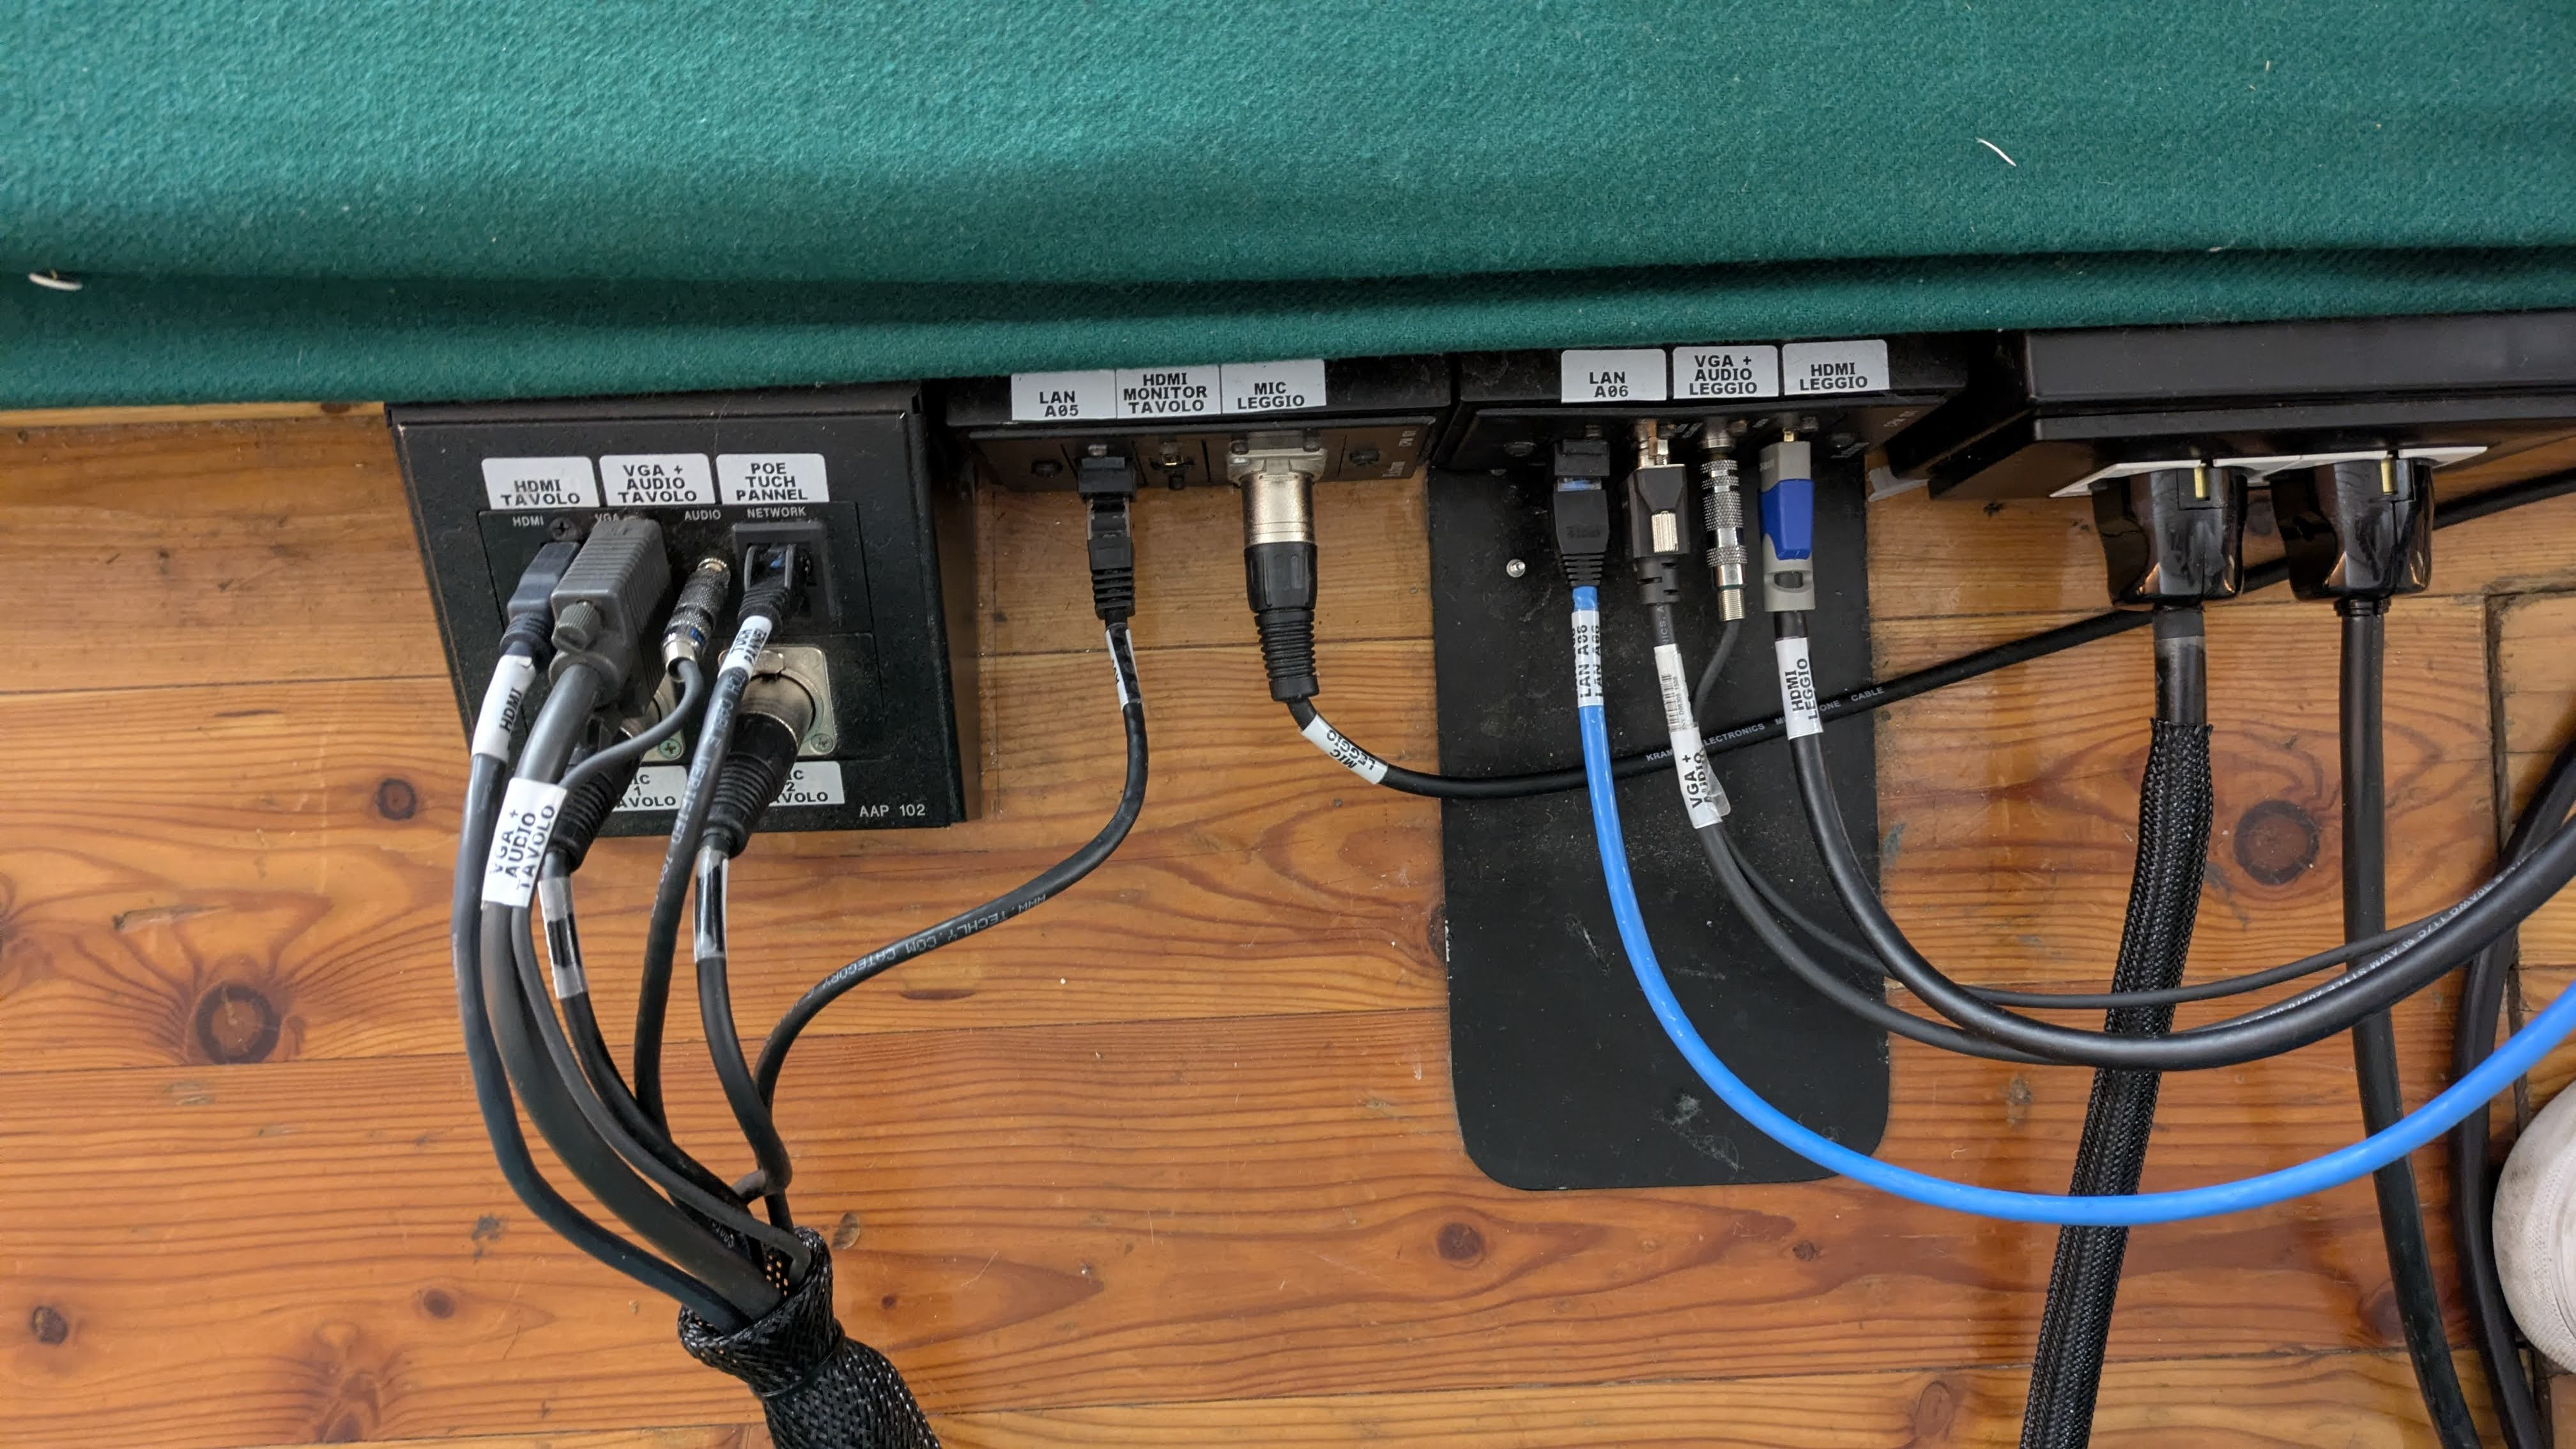
\includegraphics[width=12cm]{imgs/caviPostazione.jpg}
                    \caption{\textit{Cavi della postazione docente all'Auditorium Fogar}}
                    \label{fig:caviFogar}
                \end{figure}
% ---------------------------------------------------------------------------------------
    \newpage
            \subsubsection{Intervento sul proiettore in Aula Magna}
                    Il quarto e ultimo intervento descritto qui riguarda il proiettore presente in Aula Magna, presso il Polo di Santa Chiara. Il proiettore, collegato all'impianto tramite il controller multimediale, è montato a soffitto tramite una struttura apposita e, come ogni altro proiettore presente al CEGO, viene controllato dalla postazione del docente. \newline
                    Durante una lezione pomeridiana, mi è stato segnalato che il proiettore presentava degli artefatti visivi (\textit{Figura 4.3}) quando veniva collegato un portatile in dotazione ai Docenti; data la presunta natura del problema, la soluzione più rapida è stata quella di spostare la lezione in un'altra aula disponibile con impianto funzionante. Dopo numerosi cicli d'avvio e aver verificato se il problema persisteva anche sull'ingresso VGA, ho comunicato alla Direzione la necessità dell'intervento di un altro Tecnico. \newline
                    Questo primo intervento da parte del Tecnico esterno si è tradotto in un reset della configurazione del proiettore tramite il telecomando e, dopo svariati tentativi, gli artefatti visivi si sono risolti; ho chiesto al personale addetto alla Portineria, con cui si è interfacciato il Tecnico per orientarsi all'interno del Polo di Santa Chiara, la conferma della presenza del telecomando del proiettore presente in Aula Magna in caso di problemi futuri. \newline
                    Due giorni dopo l'intervento del Tecnico il problema è riemerso e, dopo un mio primo controllo tramite diversi cicli d'avvio e la verifica di entrambe le sorgenti, ho notato che il problema questa volta compariva anche se ci si collegava tramite l'uscita VGA (\textit{Figura 4.4}); ho contattato la Direzione avvisando del problema riemerso e di come si fosse "espanso" anche all'altro ingresso. Ho suggerito che, nella peggiore delle ipotesi, si dovesse cambiare l'intero proiettore dato che sembrava essere un problema hardware più che software. Il giorno successivo all'apertura del ticket, il Tecnico ha deciso di cambiare il commutatore collegato al controller Extron (\textit{Figura 4.5}) visto il guasto ad entrambe le uscite video; dopo un riavvio dell'impianto e dopo aver verificato il suo funzionamento collegandosi con un computer prima alla sorgente HDMI e successivamente alla sorgente VGA e infine ad entrambe contemporaneamente con due dispositivi diversi, il Tecnico ha rimosso il dispositivo precedente, lasciando il proiettore acceso in modalità stand-by, facendo notare che l'artefatto non comparirà più. 

            \begin{figure}[htbp]
                \centering
                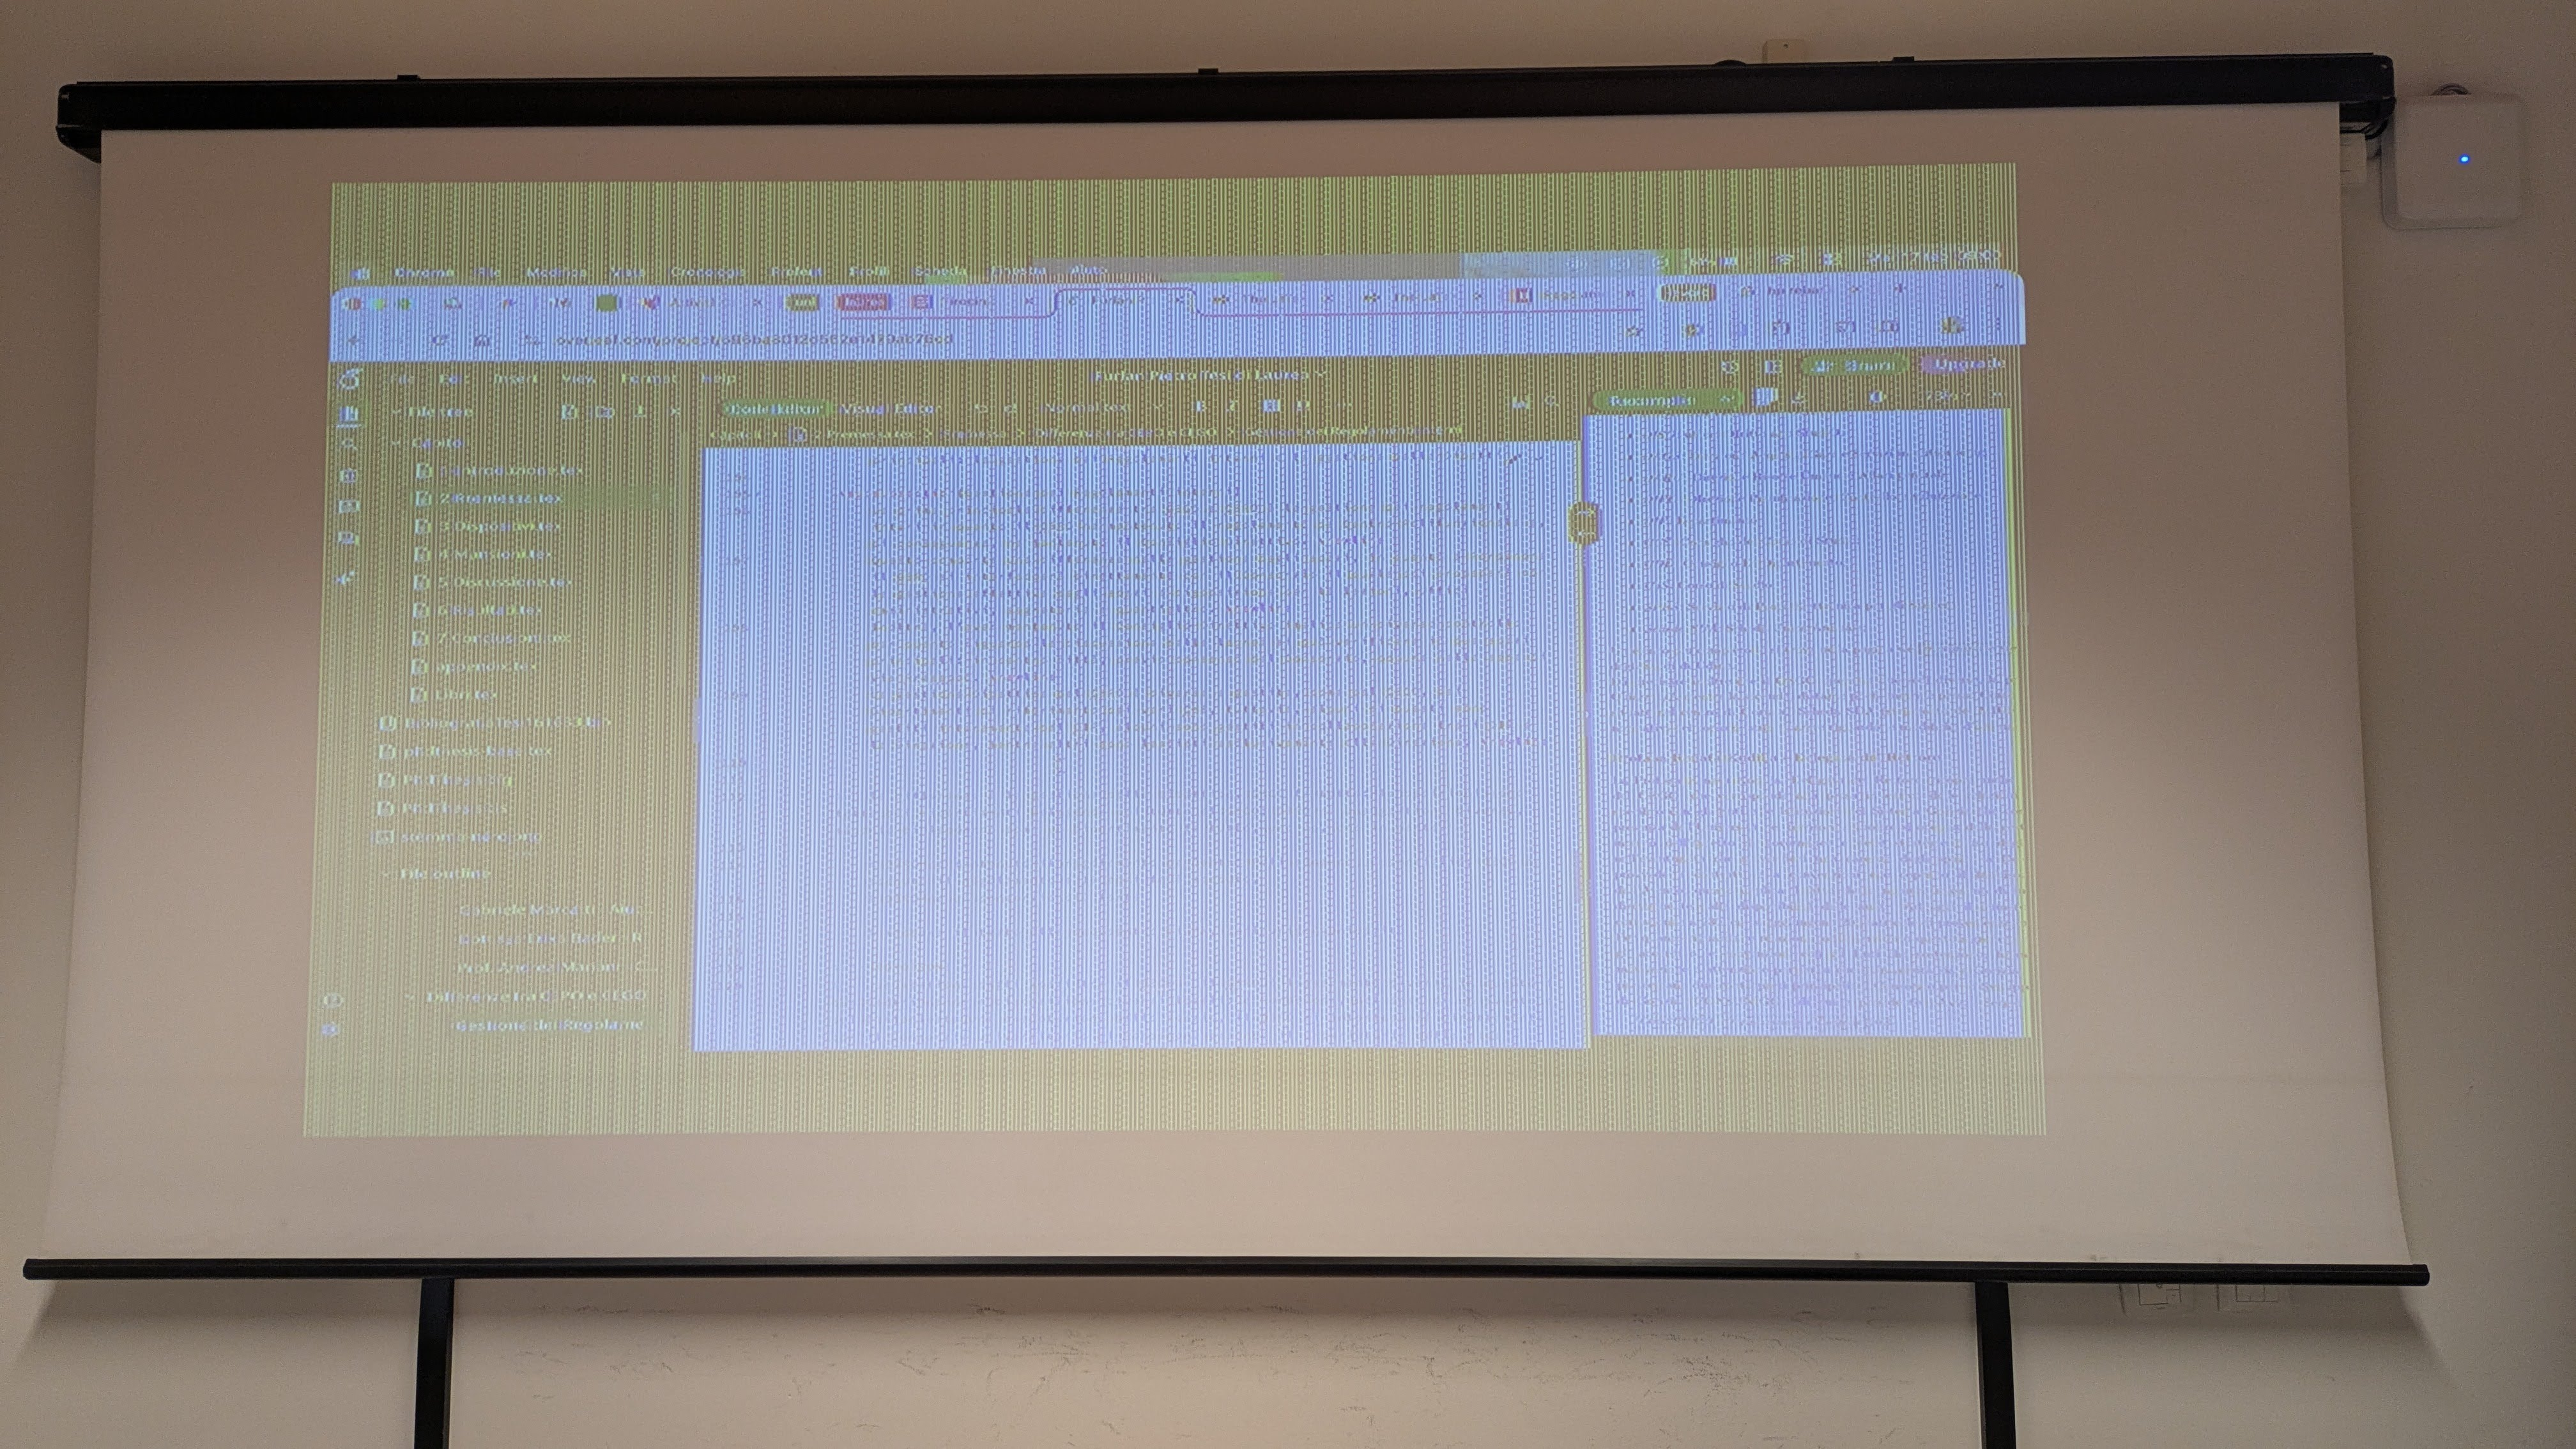
\includegraphics[width=12cm]{imgs/MagnaHDMI.jpg}
                \caption{\textit{Proiettore con collegamento HDMI}}
                \label{fig:HDMIBad}
            \end{figure}
            
            \begin{figure}[htbp]
                \centering
                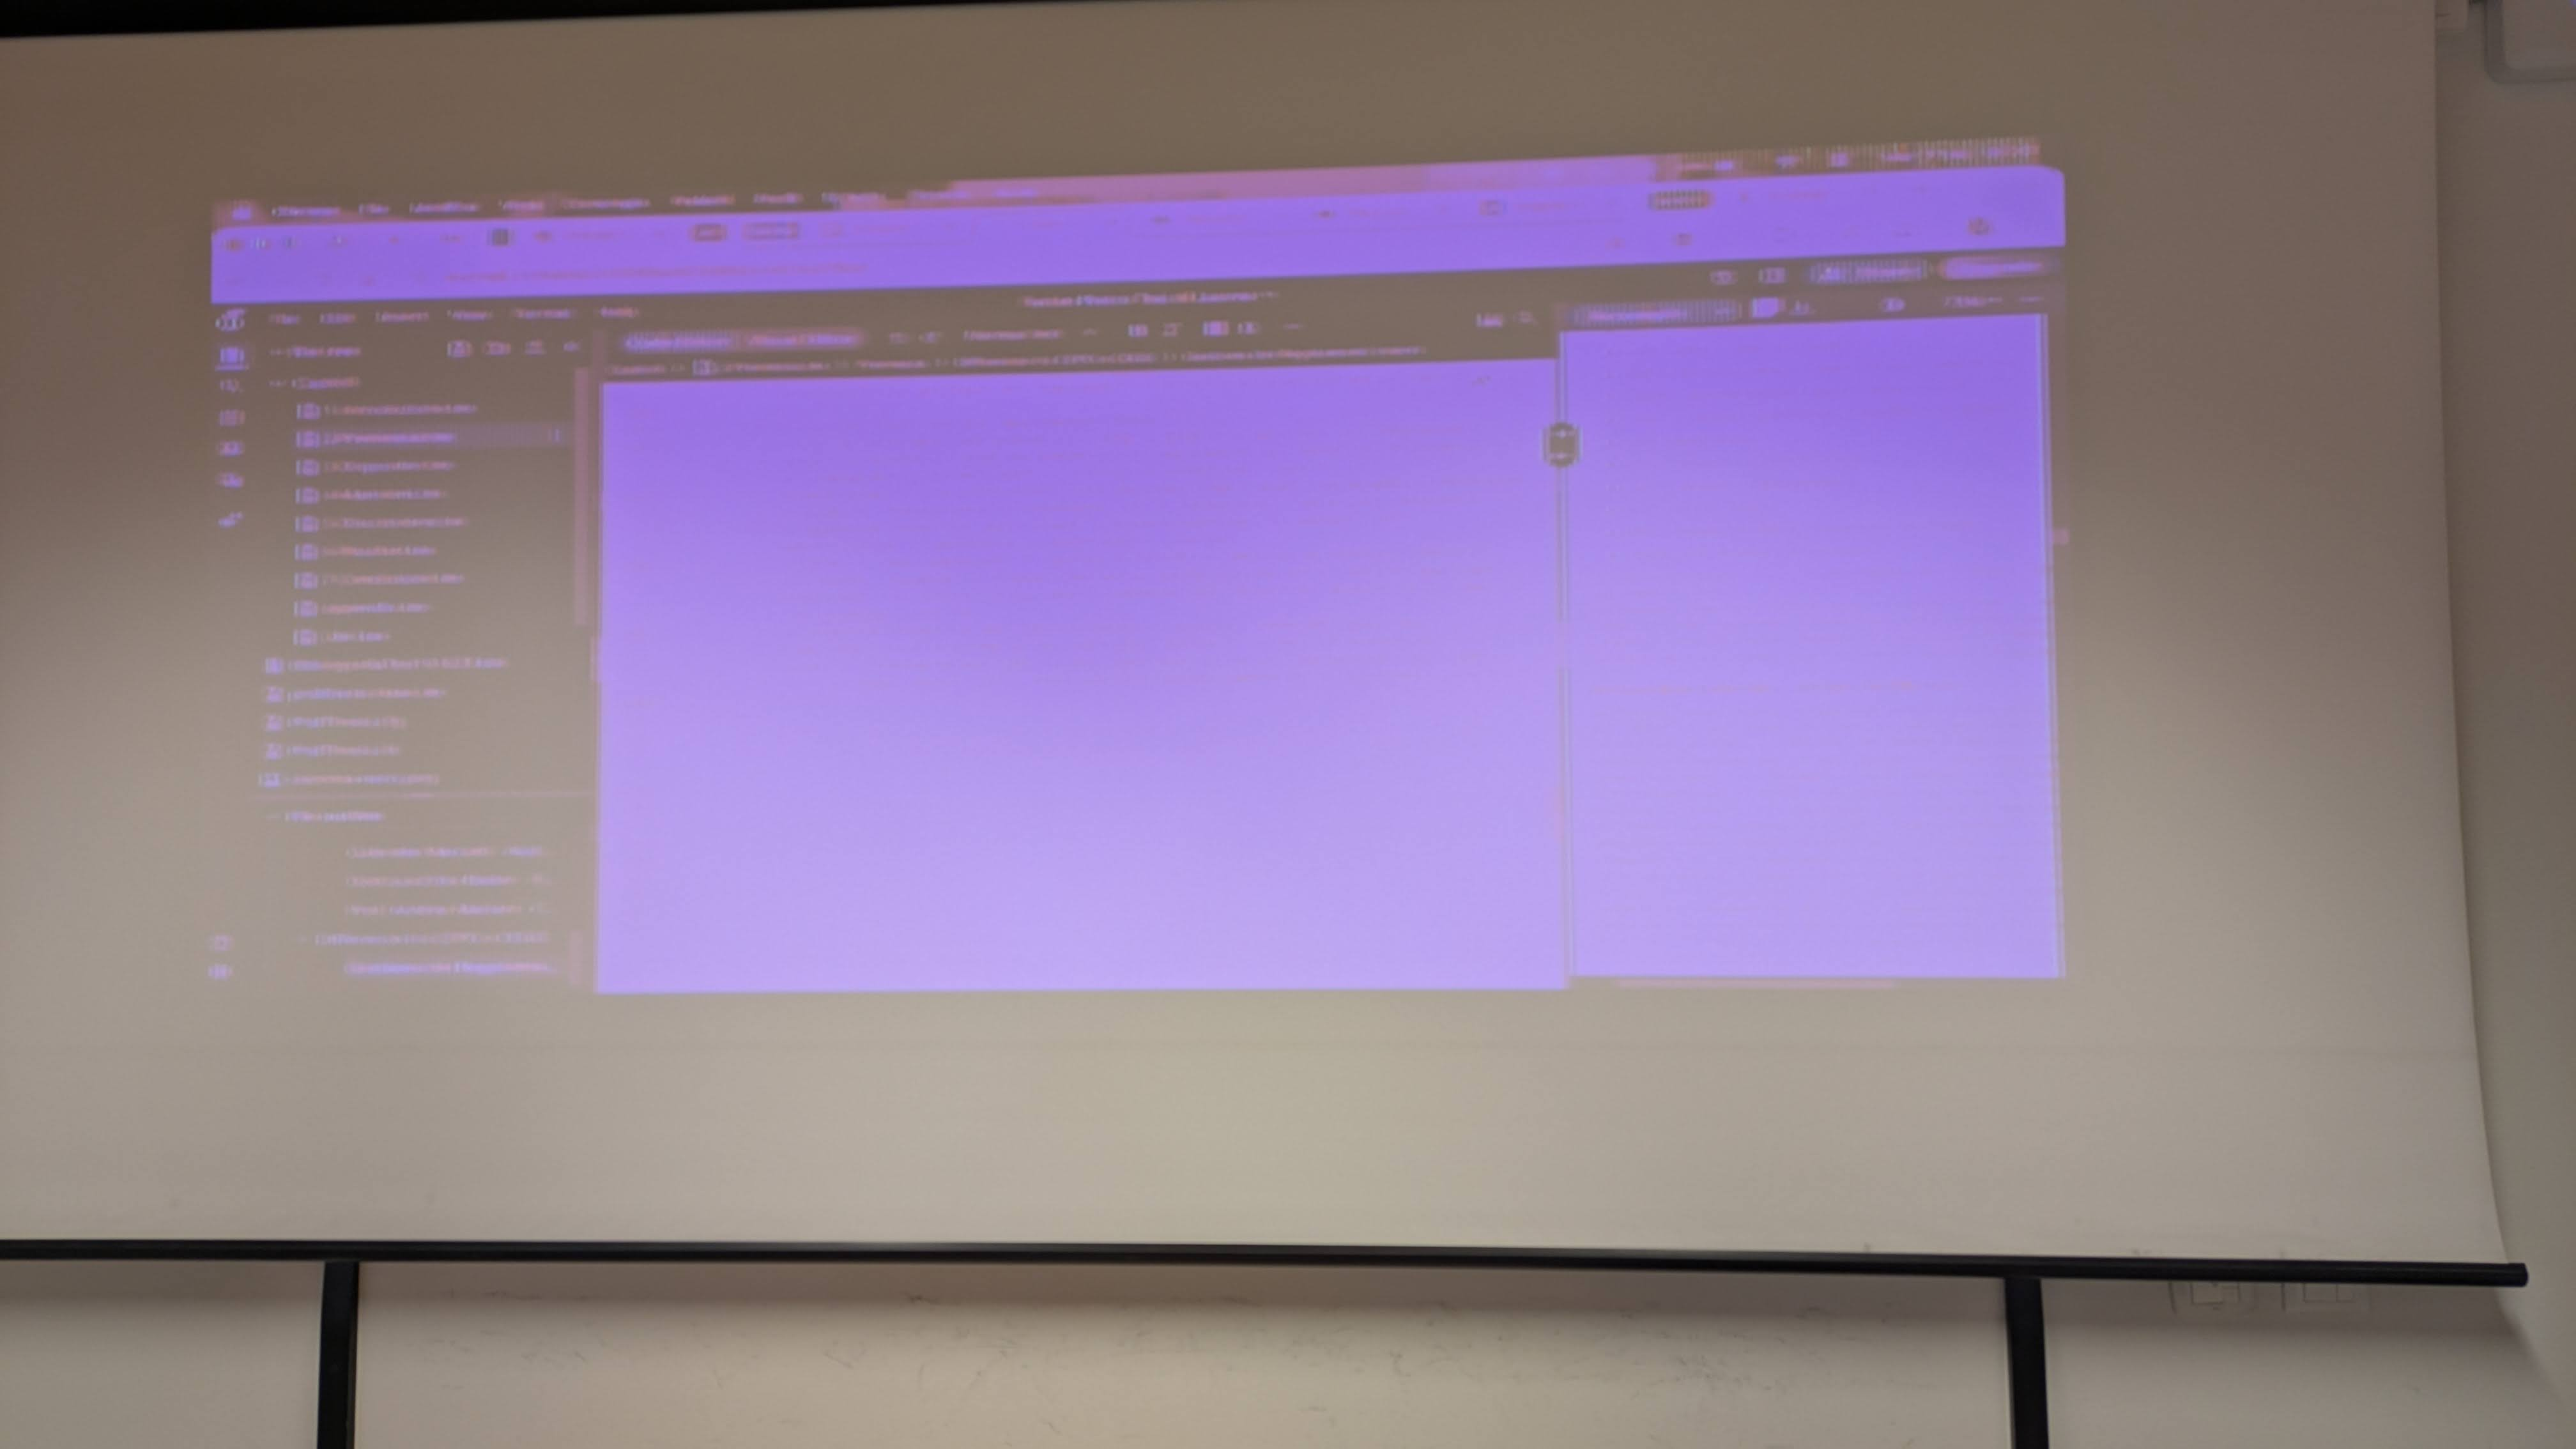
\includegraphics[width=12cm]{imgs/MagnaVGA.jpg}
                \caption{\textit{Proiettore con collegamento VGA}}
                \label{fig:VGABad}
            \end{figure}

            \begin{figure}[htbp]
                \centering
                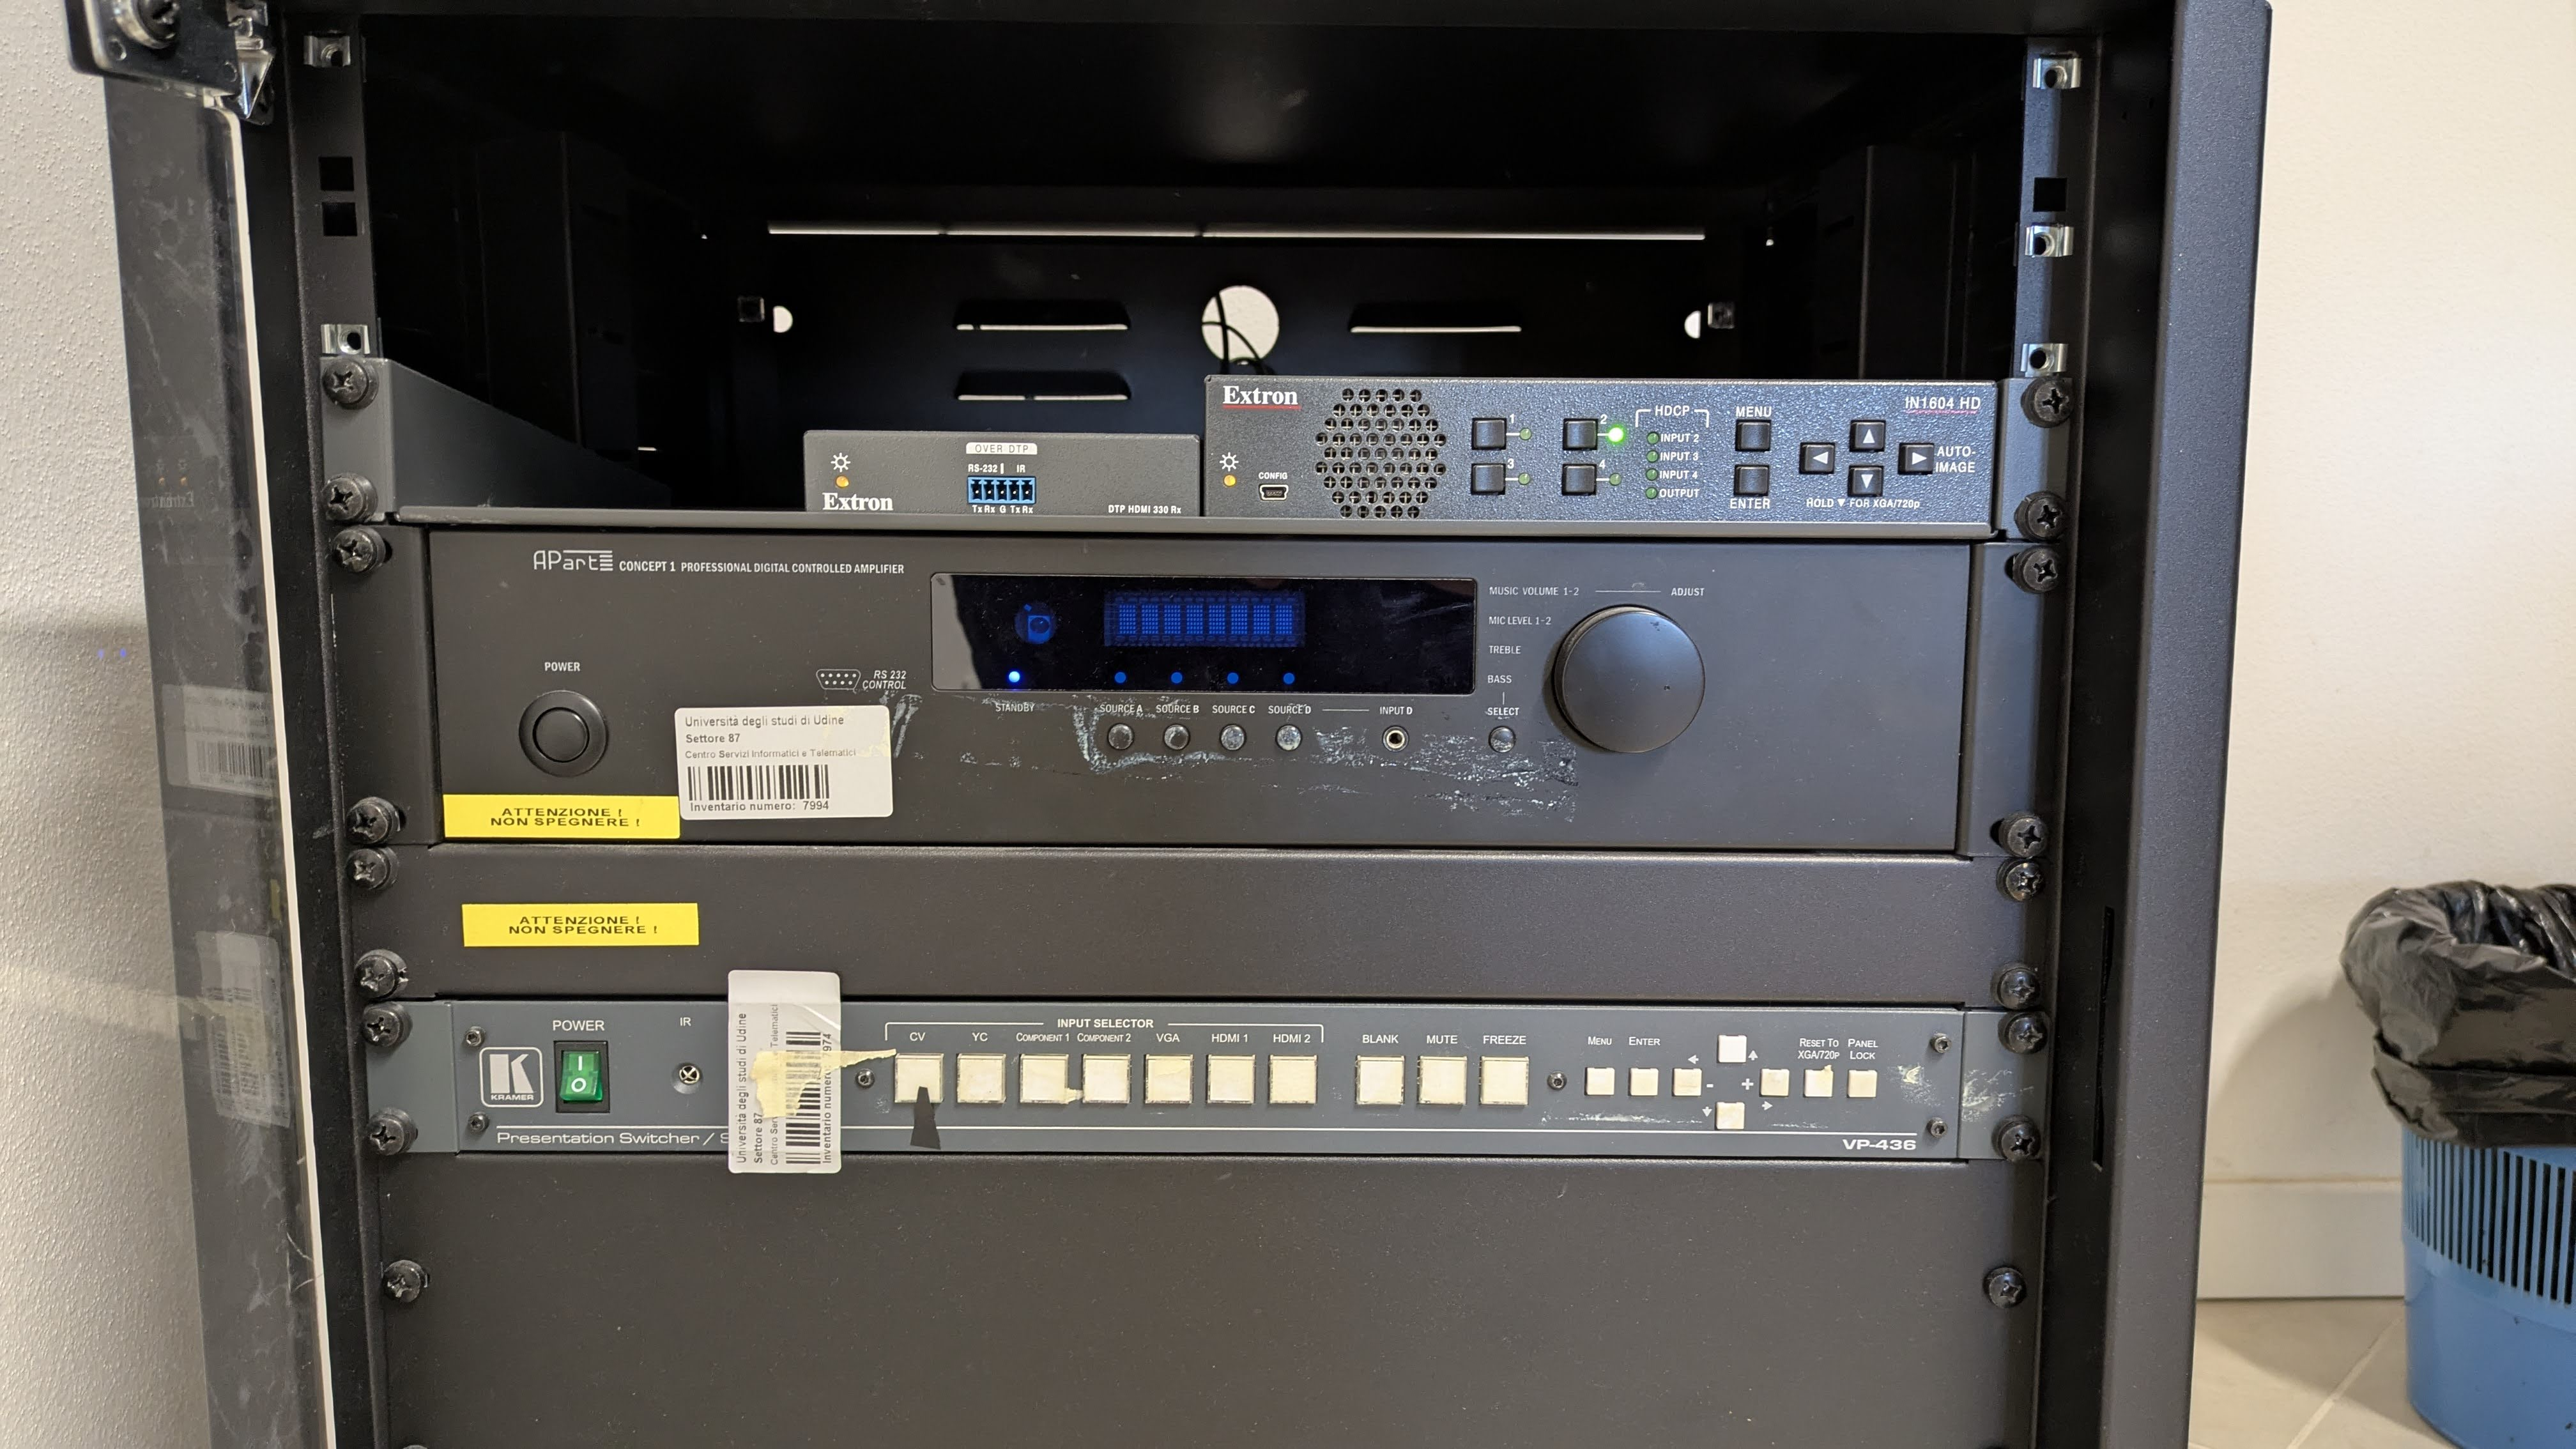
\includegraphics[width=12cm]{imgs/ArmadidettoImpiantoAudio.jpg}
                \caption{\textit{Armadietto contenente commutatore video e amplificatore}}
                \label{fig:armadietto}
            \end{figure}
    \newpage     
% ---------------------------------------------------------------------------------------
        \hfill
        \section{Altre Mansioni}
            \par
                Durante il periodo di tirocinio, mi è stato assegnato il compito di tenere traccia degli eventi costruendo, sulla base di un catalogo già esistente, un file dove si potessero segnalare i dati principali degli eventi, in modo da poter poi stipulare un report dettagliato a fine Anno Accademico. \newline
                In parallelo alla gestione degli eventi, ogni settimana per ogni giovedì, sono stato il referente per le problematiche riscontrate dalla Portineria e per le problematiche relative alla Portineria: è stato mio compito catalogare tutte le segnalazioni fatte in un file preesistente, gestito dalla Dirigente Amministrativa; questo file è stato compilato e quindi spedito a chi di competenza con cadenza settimanale. 
% ---------------------------------------------------------------------------------------
    \setcounter{chapter}{4}
\setcounter{section}{0}

\chapter{Scenari futuri}
        Con l'avvento dell'Intelligenza Artificiale (IA) si sono sviluppate molte tecnologie prima ritenute impensabili, inoltre si sono semplificate molte procedure che in passato richiedevano operazioni complesse e in generale, ci sono molti nuovi servizi disponibili; molti software stanno investendo in agenti IA che possono aiutare l'utente a svolgere i suoi compiti, una sorta di assistente digitale. Nell'ambito dell'informatica è nata una nuova tipologia di programmazione il \textit{vibe coding}, ovvero descrivere l'applicazione che si vuole realizzare ad una IA e lasciare tutta la fase di scrittura del codice e creazione della logica ad essa, alcuni esempi possono essere Claude AI, Base44 e Nothing Essential Apps. Tuttavia il dibattito sulla vera utilità delle IA è sempre più animato: in molti hanno espresso il loro timore riguardo alla possibilità di perdere il posto di lavoro venendo soppiantati da IA. L'esempio più eclatante è dato dal movimento "Anti-AI" per quanto riguarda la generazione di immagini tramite IA Generative, ponendo in evidenza come questo sia ai limiti del plagio e furto, dato che i modelli che tutt'ora utilizziamo sono stati addestrati su una mole più che significativa di dati trovati online. 
    \par
        Per quanto riguardano le IA "tecniche" ovvero i vari \textit{Large Language Model} (\textit{LLM}) specializzati nella risoluzione di problemi matematici e problemi di programmazione, bisogna riconoscere che questi sono molto utili nel cercare soluzioni rapide a problemi complessi. Tuttavia ad oggi la loro accuratezza lascia ancora a desiderare, poiché molte delle soluzioni che propongono, soprattutto nei casi di risoluzione di codice, prevedono richiami a librerie inesistenti, errori logici, ripetizione di funzioni, operazioni inutili e molte altre operazioni non ottimizzate. \newline 
        Nel contesto di questa Tesi, la IA sarà sempre "tecnica" e può essere una salvezza come una condanna per la figura del Tecnico Informatico. 
        
    \par
        Prima di iniziare a descrivere quali possono essere le caratteristiche sia del Tecnico Informatico che le caratteristiche della IA, è necessario illustrare come del semplice codice può diventare una IA.\newline
    \par
        Quello che comunemente viene chiamato Intelligenza Artificiale è una branca dell'informatica che a sua volta si suddivide in molteplici materie, tra cui il \textit{Machine Learning}. Questa materia studia programmi, algoritmi e sistemi che possono "ragionare" come un essere umano: il sistema riceve degli input e, dopo un processo che viene chiamato addestramento, genera degli output calcolati da una serie di regole generate automaticamente. Esiste un'altra materia contenuta interna al \textit{Machine Learning}, ovvero il \textit{Deep Learning} dove i singoli algoritmi hanno reti neurali molto complesse che apprendono nuovi "metodi di ragionamento e adattamento" da una grande mole di dati eterogenei. \newline
        Prendendo spunto dalla natura, lo psicologo americano Frank Rosenblatt progetta il componente fondamentale di una rete neurale informatica: il \textit{perceptron}. Questa cellula ha una struttura simile a quella del neurone, molti ingressi, un nucleo e un singolo output; questo componente base elabora gli input forniti associandoli ad un peso che determina lui, nella fase dell'apprendimento. \newline
        Il perceptron ha un limite, può solamente risolvere problemi che sono linearmente scomponibili; per rimuovere questa limitazione, vengono inseriti più perceptron in serie creando così un \textit{perceptron multi-layer} (MLP). Espandendo questo ragionamento a più livelli si ottengono le attuali reti neurali, molti livelli che risolvono dei problemi scomposti dai neuroni precedenti. I livelli sono principalmente tre: il livello di input, ovvero i primi neuroni a ricevere i dati, il livello nascosto, la moltitudine di neuroni che eseguono le operazioni intermedie, e infine il livello di output, l'ultimo livello della rete neurale che fornisce poi il risultato finale.
    \par
        Le reti neurali possono funzionare secondo due tecniche principali, in base al loro scopo: la tecnica di regressione e la tecnica di classificazione. La tecnica di regressione ha lo scopo di fornire dei risultati predittivi in funzione dell'input; la tecnica di classificazione invece ha lo scopo di classificare il risultato in base agli input forniti. \newline
        Per poter scegliere la tecnica giusta bisogna prima definire il ciclo di vita di una rete neurale. Il ciclo è diviso in 5 fasi, la prima fase è la definizione della tecnica da usare in base alla tipologia di problema in cui si vuole applicare la rete neurale. La seconda fase riguarda invece la raccolta e la preparazione dei dati, normalizzandoli, in modo da non avere anomalie e migliorare l'efficienza dell'apprendimento; è importante che si scelga o si crei una mole di dati sufficientemente grande e sufficientemente eterogenea. La terza fase riguarda la configurazione del modello, scegliendo il numero di input, secondo anche i dati scelti precedentemente, e quali output deve fornire. Successivamente la quarta fase riguarda l'apprendimento, ovvero un processo iterativo dove la rete "impara" in base ai dati forniti; questa fase può essere supervisionata, con un'entità che ha l'output corretto e quindi può verificarne il risultato finale, oppure non supervisionato, lasciando la rete neurale agli output che crea; l'apprendimento non supervisionato è usato se non si dispongono dei risultati nel dataset fornito alla IA. Esiste anche l'apprendimento per rinforzo, ovvero che la rete neurale apprende in base a scenari reali o simulati, visualizzando le decisioni come ricompense o penalità, massimizzando poi le ricompense. \newline
        Infine, l'ultima fase del ciclo di vita riguarda la valutazione e successiva ottimizzazione della rete neurale; una volta terminata la fase di ottimizzazione, si può ripetere il ciclo ripartendo dall'addestramento della rete ottimizzata, proseguendo fino a che la rete ha raggiunto il grado di accuratezza richiesto\footnote{\cite{NeuralNetworks}}. 
    \par
        Un metodo alternativo alla creazione di una rete neurale è la neuroevoluzione; anche questo metodo prende spunto dalla natura con la mutazione casuale di geni, in questo contesto la mutazione casuale è un algoritmo di generazione randomica di valori numerici mentre i geni sono i pesi associati ad ogni input del singolo neurone. \newline
        La neuroevoluzione, oltre a gererare randomicamente i pesi tra più agenti, testa la rete neurale in un ambiente e poi ne viene valutato l'adattamento; in base alla valutazione, il neurone più adatto tramanda i suoi pesi a nuovi agenti generati e, questi pesi, subiscono una mutazione. \newline
        Questo tipo di creazione della rete neurale è utile se i risultati che si vogliono ottenere non hanno delle regole ben definite e chiare, tramite questo metodo, la rete impara facendo e arriverà ad un risultato ottimale\footnote{\cite{Neuroevolution}}. 
% ---------------------------------------------------------------------------------------
        \section{Le caratteristiche del Tecnico in loco}
            \par
                Come si può evincere da quanto fin qui esposto, la presenza in loco di un Tecnico Informatico è pressoché fondamentale per garantire la corretta erogazione del servizio, in questo caso universitario, situazione non possibile con una IA. \newline
                Un buon Tecnico sempre presente riuscirà sempre a portare a termine un intervento senza "esaurire i token" o dover rimandare a causa di un "sovraccarico del server" o per "indisponibilità del server". 
            \par
                Facendo riferimento agli interventi eseguiti, molti di questi potrebbero essere sì facilmente eseguibili dalle IA, ma bisogna prendere atto che queste non riuscirebbero ad agire in autonomia: per esperienza personale, la sola IA che riesce per ora a interagire con diversi applicativi è Google Gemini ma le app sono solamente quelle che Google mantiene aggiornate, oltre al fatto che molte delle funzionalità più avanzate sono bloccate da un abbonamento mensile. Molti dei modelli in commercio e d'uso anche quotidiano forniscono solamente una risposta, quasi sempre a favore di ciò che gli si chiede, fornendo una sorta di riassunto di diversa lunghezza con il suggerimento di possibili operazioni più o meno semplici.
            \par
                Bisogna sottolineare però la continua formazione da parte del Tecnico Informatico, in quanto molte delle tecnologie in uso oggi potrebbero non esserlo più tra qualche anno, un banale esempio in tal senso riguarda la Direttiva Europea che obbliga tutti i dispositivi mobili ad usare il cavo di ricarica USB tipo C, in modo da unificare i caricabatterie; entro aprile 2026 ogni portatile dovrà seguire questa normativa\footnote{\cite{DirettivaUE_2022/2380},\cite{EU-USB-C}}. 
% ---------------------------------------------------------------------------------------
        \section{Le caratteristiche delle IA}
            \par
                I vantaggi delle IA sono molteplici, tra cui sicuramente la rapidità nella risposta e la maggiore accuratezza nella risposta in relazione al prompt fornito, offrendo un'ampia gamma di molteplici soluzioni e indagando possibili cause. Hanno sicuramente uno spettro di competenze più ampio, attingendo dall'infinità di risorse che si trovano sul web, tanto che sotto numerosi punti di vista le IA possono essere considerate un'enciclopedia tascabile che permette di sapere tutto su qualsiasi tipologia di intervento. 
            \par
                Avendo molti modelli disponibili in commercio, si possono anche avere diverse "opinioni" da più modelli diversi, una sorta di consiglio decisionale, per ottenere il risultato più accurato possibile, rendendo l'intervento una sola messa in atto della risposta del consiglio delle IA.
            \par
                Tuttavia, le IA forniscono risposte che potrebbero contenere errori dovuti alla mole di dati su cui si sono addestrate e non è detto quindi che gli interventi proposti siano effettivamente corretti e adeguati alla vera problematica in oggetto. \newline
                In aggiunta, alle IA va individuato anche un eccessivo consumo inteso nell'immediato in relazione alla banda di rete dell'Università ma a lungo termine anche in riferimento alle conseguenze climatiche che si vengono a generare nel tenere accesi tutti i data center necessari, altamente energivori; per non parlare dell'attuale crisi di mercato per quanto riguarda il reperimento di componenti dei computer: nel giro di qualche mese, i prezzi delle memorie RAM si sono moltiplicati di oltre il 300\% del loro valore e i prezzi delle memorie NVME, in generale di memorie di massa ad alte prestazioni, sono saliti del circa 50\%. \newline
                Tuttavia basti questo accenno, in quanto analisi di mercato e discussione sulle tematiche ambientali non rientrano nel focus di questa tesi di Laurea. 
            \par
                Un problema più tangibile è la formazione di tutto il personale, nel caso in cui si voglia ad esempio adottare una IA come Tecnico Informatico: ogni membro del personale dovrebbe saper costruire un prompt degno di generare una risposta quanto più accurata al problema che si sta riscontrando e ogni membro del personale dovrebbe essere formato anche sulle basi dell'informatica, sia hardware sia software. 
% ---------------------------------------------------------------------------------------
        \section{Possibili soluzioni ibride}
            \par
                Nonostante questi sviluppi, la presenza di un Tecnico è ormai fondamentale e spesso accettata come un presupposto, in quanto basta solamente un primo contatto e la procedura d'intervento si avvierà subito, senza andare a scatenare una catena di tentativi e possibili errori che nuocerebbero alla continuità di servizio e all'immagine dell'Università. \newline 
                Riflettendo sul fatto che la maggior parte degli interventi di routine hanno riguardato collegamenti errati agli impianti audiovisivi risulta evidente che eseguire richieste alla IA per ogni singolo intervento sarebbe stato oneroso in termini di tempo, sia in riferimento alla durata dell'intervento stesso sia in relazione al tempo d'attesa della risposta da parte della IA. \newline
                Di seguito si possono trovare tre ipotesi di collaborazione a questa situazione, in cui il Tecnico si ritrova a convivere con uno strumento sempre più d'uso comune. 
% ---------------------------------------------------------------------------------------
            \subsection*{Collaborazione Pura 50 Tecnico - 50 IA}
                La prima ipotesi tende più a uno scenario ideale, ossia a una collaborazione pura tra il Tecnico e la IA. In questa situazione, la IA fornisce informazioni e suggerimenti su procedure e interventi mentre il Tecnico, oltre a eseguire l'intervento vero e proprio, pondera con cautela ciò che gli viene suggerito filtrando eventuali soluzioni multiple fornite dalla singola risposta della IA. Questo non solo renderebbe più rapidi gli interventi ma risolverebbe anche il problema delle piattaforme eterogenee presenti all'interno di quello che è un campus universitario.
% ---------------------------------------------------------------------------------------
            \subsection*{Collaborazione 70 Tecnico - 30 IA}
                La seconda ipotesi invece è più reale, dove il bilanciamento viene spostato verso l'esperienza del Tecnico. Non appena si verifica un problema che richiede un intervento, il Tecnico procede immediatamente a risolverlo in base alle sue conoscenze pregresse e informazioni che gli vengono fornite tramite il ticket di assistenza; solo nel caso in cui l'intervento si riveli più complesso del previsto, il Tecnico potrà consultare la IA formulando un prompt ben preciso, costruito sui tentativi già eseguiti, e provando ad applicare quanto gli viene proposto dalla riposta della IA. 
% ---------------------------------------------------------------------------------------
            \subsection*{Collaborazione 30 Tecnico - 70 IA}
                L'ultima ipotesi è la più improbabile: prevede un quasi completo affidarsi alla IA per la maggior parte degli interventi di ordinaria manutenzione, lasciando solamente gli interventi più delicati e complessi al Tecnico. Questo farebbe in modo da alleggerire sia l'aspetto delle responsabilità in caso di danni che l'aspetto della quantità di lavoro e quindi la suddivisione degli interventi in più giornate lavorative. \newline
                La IA, in questo caso, non potrà avere accesso ai file privati del personale, in quanto violerebbe i diritti sulla privacy. 
% ---------------------------------------------------------------------------------------
            \hfill
            \par
                Tali scenari e ipotesi di collaborazione possono funzionare solamente nel caso in cui la IA sia stata ben addestrata su una mole di dati eterogenea e soprattutto nell'ambito informatico e delle telecomunicazioni; questo ambito è in continuo e rapido sviluppo ma i parametri fondamentali e le tecniche d'intervento sono pressoché rimaste invariate. Parimenti gli interventi d'ordinaria manutenzione possono risultare spersonalizzanti e lasciarli in carico ad uno strumento automatizzato può migliorare la qualità complessiva degli interventi svolti. \newline
                Fare affidamento dunque a uno strumento così potente che permette, non solo semplificare i lavori di manutenzione, ma anche di sostituire l'intervento del Tecnico è sicuramente un passo nella giusta direzione; l'importante è che la figura del Tecnico non solo non venga completamente scalzata dalle nuove tecnologie ma anche che egli stesso sia in grado di filtrare con cura ciò che gli viene fornito come risposta e come "soluzione assoluta" dalla IA.
% ---------------------------------------------------------------------------------------
    \setcounter{chapter}{5}
\setcounter{section}{0}

\chapter{Esiti}
    Le seguenti sezioni illustrano come il Corso di Studio in Scienze e Tecnologie Multimediali possa creare una figura tecnica professionale e di come possa preparare ai vari dispositivi multimediali e informatici che si possono trovare in un Polo Universitario. \newline
    Viene poi dedicata una sezione ai possibili sbocchi lavorativi nelle P.A., nello specifico nella Scuola Secondaria di Secondo Grado e nelle Università. 
% ---------------------------------------------------------------------------------------
    \section{Preparazione del Corso di Studio}
        Avendo ottenuto il Diploma di Informatica e Telecomunicazioni, non sono un estraneo al mondo dell'informatica; nonostante tale formazione di base ho potuto personalmente esprimere come l'offerta formativa del CdS sia molto buona, fornendo un'efficace preparazione a tutte quelle casistiche al limite tra l'informatica e il multimediale che ho riscontrato durante il periodo di tirocinio presso il CEGO. \newline 
        Ho notato maggior focus da parte del CdS nelle materie tecniche e laboratoriali, soprattutto sull'insegnamento Laboratorio di Programmazione e Sistemi Multimediali sostenuto con il Docente e mio Relatore Prof. Niki Martinel in quanto tale percorso mi ha dato una preparazione superiore rispetto ad altri insegnamenti, sempre di natura tecnica. \newline
        Poiché l'Insegnamento tratta sia di programmazione e sviluppo di applicativi sia che di sistemi multimediali, veniva a essere toccato ogni aspetto tecnico che si possa immaginare: la parte riguardante i sistemi multimediali ha illustrato con cura il punto di vista storico-tecnologico dell'informatica, mentre la seconda parte ha fatto riferimento  più su strutture dati e algoritmi da sviluppare in un linguaggio ad alto livello, Python. Questo approccio multiplo della materia mi ha aiutato a capire meglio come funzionano molti applicativi e soprattutto mi ha aiutato a capire le strutture dei vari file, degli algoritmi e la manipolazione di dati e formati multimediali e come questi dati vengono gestiti dal software; durante il tirocinio mi ha aiutato a identificare meglio alcuni problemi con cui mi sono dovuto misurare. \newline
        I testi di studio inoltre mi hanno guidato non solo nella preparazione all'esame ma anche durante il periodo di tirocinio, illustrandomi le diverse tecnologie e i diversi meccanismi su cui non solo si fonda l'informatica di oggi ma che si trovano ormai ovunque.
        \par
            Durante il periodo di tirocinio ho avuto modo di conoscere diversi aspetti della vita universitaria, prima sconosciuti: ho vissuto di prima mano cosa vuol dire lavorare nell'Amministrazione di un Polo Universitario e nello specifico ho potuto cimentarmi nelle mansioni di un Tecnico Informatico. \newline
            Questo tirocinio mi ha aiutato ad ampliare le mie conoscenze tecniche e mi ha permesso di migliorare quei aspetti professionali che prima non avevo approfondito, data la natura scolastica del mio percorso. I ritmi che in alcuni momenti definirei frenetici degli interventi mi hanno dato una prospettiva nuova, prima sconosciuta, delle possibilità lavorative post-laurea. Mi ha anche permesso di ampliare i miei orizzonti per quanto riguarda altri possibili sbocchi lavorativi nel pubblico, piuttosto che nel privato. 
% ---------------------------------------------------------------------------------------
    \section{Inserimento Professionale}
        \par
            Gli inserimenti professionali possibili sono molteplici e possono variare di molto in base a ciò in cui mi poteri specializzare. Inizialmente, l'obiettivo era quello di proseguire immediatamente gli studi attraverso il conseguimento di una Laurea Magistrale ma, dopo il periodo di Tirocinio, mi sono ritrovato di fronte ad un bivio: proseguire gli studi e rimandare l'ingresso nel mondo del lavoro oppure dare in un certo senso prosecuzione all'attività di tirocinio, puntando ad un posto di lavoro come tecnico informatico. 
        \par
            Tutt'ora il proseguire gli studi costituisce una forte spinta motivante a trovare un posto di lavoro che mi permetta di conciliare entrambe le possibilità: da qui nasce il desiderio di lavorare nelle Pubbliche Amministrazioni, attraverso la partecipazione a diversi bandi sia nell'ambito delle Scuole Secondarie di Secondo Grado o magari nell'ambito della stessa Università di Udine.
        \par
            Per quanto riguarda il profilo di Tecnico Informatico presso l'Università, i bandi vengono pubblicati in una sezione apposita presente nel sito web, dove vengono catalogati e raggruppati per Dipartimento richiedente; nello specifico, l'ente universitario \cite{DARU}.
        \par
            Per le Scuole Secondarie di Secondo Grado, i posti di lavoro disponibili per un neo-laureato triennale sono principalmente due: Personale ATA di 3a Fascia e Insegnate Tecnico Pratico per la cattedra B016. \newline
            Per il profilo ATA di Assistente Tecnico il requisito di base è ancora il solo Diploma di Scuola Secondaria di Secondo Grado corrispondente allo specifico settore professionale unito alla Certificazione Internazionale di Alfabetizzazione digitale, come previsto dal \cite{CCNL-Istruzione/Ricerca}, entrato in vigore 1 maggio 2024. Tuttavia la Laurea Triennale è un titolo valutabile utile ad ottenere un punteggio aggiuntivo. Per il Personale Tecnico Amministrativo (PTA) in ambito universitario si fa riferimento al D.Lgs. 165/2001, CCNL Funzioni Centrali/Istruzione e Ricerca e al regolamento interno dell'Università.\newline
            La Laurea Triennale per gli Insegnanti Tecnico-Pratici (ITP) è stata invece stabilita dal \cite{D.L.59/2017} tuttavia la sua entrata in vigore è stata prorogata, spostando il termine ultimo dall'iniziale 2025 al 31 dicembre 2026 con il \cite{DecretoMilleproroghe}. A partire da tale termine, serviranno la Laurea Triennale oltre ai 24 CFU/CFA per accedere ai concorsi, mentre finora è stato sufficiente il solo Diploma di Scuola Secondaria di Secondo Grado. 
        \par
            Il percorso appena sopra delineato può sembrare accidentato e complesso ma risulta essere altamente poiché può dar luogo a una figura professionalmente qualificata, permettendo quasi di "chiudere un cerchio" andando virtualmente a congiungere le materie oggetto di studio all'ambiente in cui questo si è svolto, come può esserlo la scuola o l'Università. \newline
            Il percorso lavorativo risulta invece essere indubbiamente diverso nell'ambito privato, in quanto le aziende tendono a cercare figure specializzate, ad esempio sistemisti o sviluppatori, oppure Tecnici manutentori o \textit{Information Technology} (IT), che operino molto più spesso di quanto accada nell'ambito dei servizi pubblici nelle fasce orarie in cui l'azienda sia vuota allo scopo di non interromperne la produttività e diminuendo in tal modo fortemente l'interazione interpersonale con il capitale umano. 
% ---------------------------------------------------------------------------------------   
    \backmatter
    \conclusions\label{ch:concl}
    \par
        Questa Tesi di laurea mirava a fare luce sulla figura e sul ruolo del Tecnico Informatico all'interno di un Polo Universitario, ruolo che spesso viene trascurato nel settore nonostante sia un ruolo chiave per garantire la continuità dei servizi TIC offerti dalle Università, oltre che da qualsiasi altra istituzione, in un mondo ormai sempre più digitalizzato e tecnologico. 
    \par
        Durante questo periodo di tirocinio ho vissuto a stretto contatto con la Direzione del Centro Polifunzionale di Gorizia, interfacciandomi anche con i tecnici del DAGS per poter fare interventi specifici su loro richiesta. Questa esperienza mi ha permesso di lavorare in un ambiente familiare ma, da un altro punto di vista, mi ha permesso anche di approfondire scenari e situazioni che prima mi erano sconosciuti. Il tirocinio mi ha permesso di mettere in gioco le mie abilità non solo tecniche ma anche di adattamento e di gestione degli interventi, in quanto molto spesso le decisioni tecniche dovevano essere prese nell'arco di qualche minuto. \newline
        Le mansioni ricoperte erano state precedentemente illustrate in occasione di un colloquio conoscitivo avvenuto prima dell'avvio del tirocinio, tuttavia queste si sono ampliate in corso d'opera. Il Corso di Studi in Scienze e Tecnologie Multimediali, attualmente Corso di Studi in Tecnologie digitali e comunicazione per le industrie creative, mi ha fornito delle conoscenze più che approfondite in molte aree e mi ha permesso di affrontare tutti i compiti richiesti e ciò che di nuovo ho potuto sperimentare. 
    \par
        Dato il rapido sviluppo delle nuove tecnologie, nello specifico dell'Intelligenza Artificiale, mi è sembrato opportuno discutere della figura del Tecnico anche ponendola a confronto con le IA e di come questi due diversi soggetti possano convivere ed esistere. Le IA offrono una maggiore rapidità di risposta a discapito però dell'accuratezza, mentre il Tecnico Informatico può intervenire sempre, garantendo il corretto funzionamento del dispositivo. 
        Da questo tirocinio ho appreso inoltre che la componente fondamentale di qualsiasi intervento, oltre alle conoscenze pregresse, è il sapersi interfacciare con l'ambiente umano e l'empatia che ne deriva; due fattori chiave che nonostante la IA possa provare a replicare, non saranno mai al pari di un qualsiasi rapporto e intervento con un Tecnico vero e proprio. 
    \par
        Infine questa esperienza mi ha permesso di accrescere le mie abilità di Tecnico Informatico, specializzandomi in interventi in loco in ambito informatico-multimediale. Il tirocinio inoltre mi ha aiutato a fare chiarezza sul mio futuro, orientandomi in direzione del lavoro preferibilmente presso le Pubbliche Amministrazioni, senza tuttavia escludere a priori l'ambito privato.

    % --- Bibliografia --- %
    \bibliography{BibliografiaTesi161633}
    \bibliographystyle{apacite}                             % Imposta lo stile della Bibliografia in base al Modello APA 6th
    \printindex
    
\end{document}
